\chapter{Esperimenti e risultati}\label{esperimenti}
In questo capitolo vengono presentati gli esperimenti condotti e si analizzano i risultati ottenuti.

\section{Descrizione dei dataset utilizzati}
\label{dataset}
Per la conduzione degli esperimenti sono stati adoperati due distinti dataset di immagini, di seguito descritti

\begin{itemize}

\item Il primo, usato per la fase di addestramento delle reti neurali, è una collezione di fotografie di tursiopi (scattate tra luglio 2016 e settembre 2017) e grampi (scattate tra luglio 2013 e agosto 2018) nel \textbf{Golfo di Taranto} (mar Ionio Settentrionale). Le fotografie sono state scattate e messe a disposizione dall'associazione \textit{Jonian Dolphin Conservation} (par. \ref{contesto}). Il dataset contiene immagini acquisite in un'area di 14000 km\textsuperscript{2} percorsa su un catamarano e seguendo rotte prestabilite.
Il dataset acquisito contiene in totale n=10194 immagini, suddivise in cartelle in base alla specie ritratta e ulteriormente ramificate in sottocartelle in base alla data degli scatti.

\item Il secondo, usato per testare le prestazioni dei classificatori binari precedentemente addestrati, consiste in un insieme di fotografie di grampi scattate nel mese di giugno 2018 nei pressi delle \textbf{Isole Azzorre} (Oceano Atlantico settentrionale) dall'associazione \textit{Nova Atlantis Foundation} (par. \ref{contesto}).
Questo dataset contiene in totale n=11290 immagini, anche questa volta suddivise in cartelle in base alla data degli scatti.
\end{itemize}

Entrambi i dataset contengono fotografie con una notevole risoluzione $6000\times 4000$, con occupazione di memoria di circa 10MB per foto e occupazione totale di circa 100GB per dataset. Tuttavia, prendendo visione delle immagini in ciascuno dei due dataset ci si rende subito conto che non tutte contengono pinne dorsali di cetacei: in alcune foto sono totalmente assenti, rendendo lo scatto totalmente privo di contenuto informativo per i biologi.
Anche laddove le pinne sono presenti, esse possono risultare sfocate o di bassa risoluzione se molto lontane, sovrapposte tra due esemplari vicini, disturbate da schizzi d'acqua o riflessi di luce. Infine, in tutte le fotografie sono inevitabilmente ritratti oggetti che non sono informativi ai fini dello studio delle sole pinne dorsali quali barche, persone, uccelli, terraferma (paesaggi), porzioni di cielo, boe, lo specchio d'acqua ma anche parti dei cetacei diversi dalla loro pinna dorsale, quali pinne caudali e laterali, il dorso e la testa degli esemplari. Alcune di queste situazioni sono mostrate in figura \ref{fig:esempiDataset}.

\begin{figure}[h]

  \centering
  
  \begin{subfigure}[b]{\textwidth}
    \includegraphics[width=0.24\textwidth]{t1.jpg}
    \hfill
    \includegraphics[width=0.24\linewidth]{t2.jpg}
    \hfill
    \includegraphics[width=0.24\linewidth]{t3.jpg}
    \hfill
    \includegraphics[width=0.24\linewidth]{t6.jpg}
    \caption{}
  \end{subfigure}
  
  \vspace{5mm}
  
  \begin{subfigure}[b]{\textwidth}
    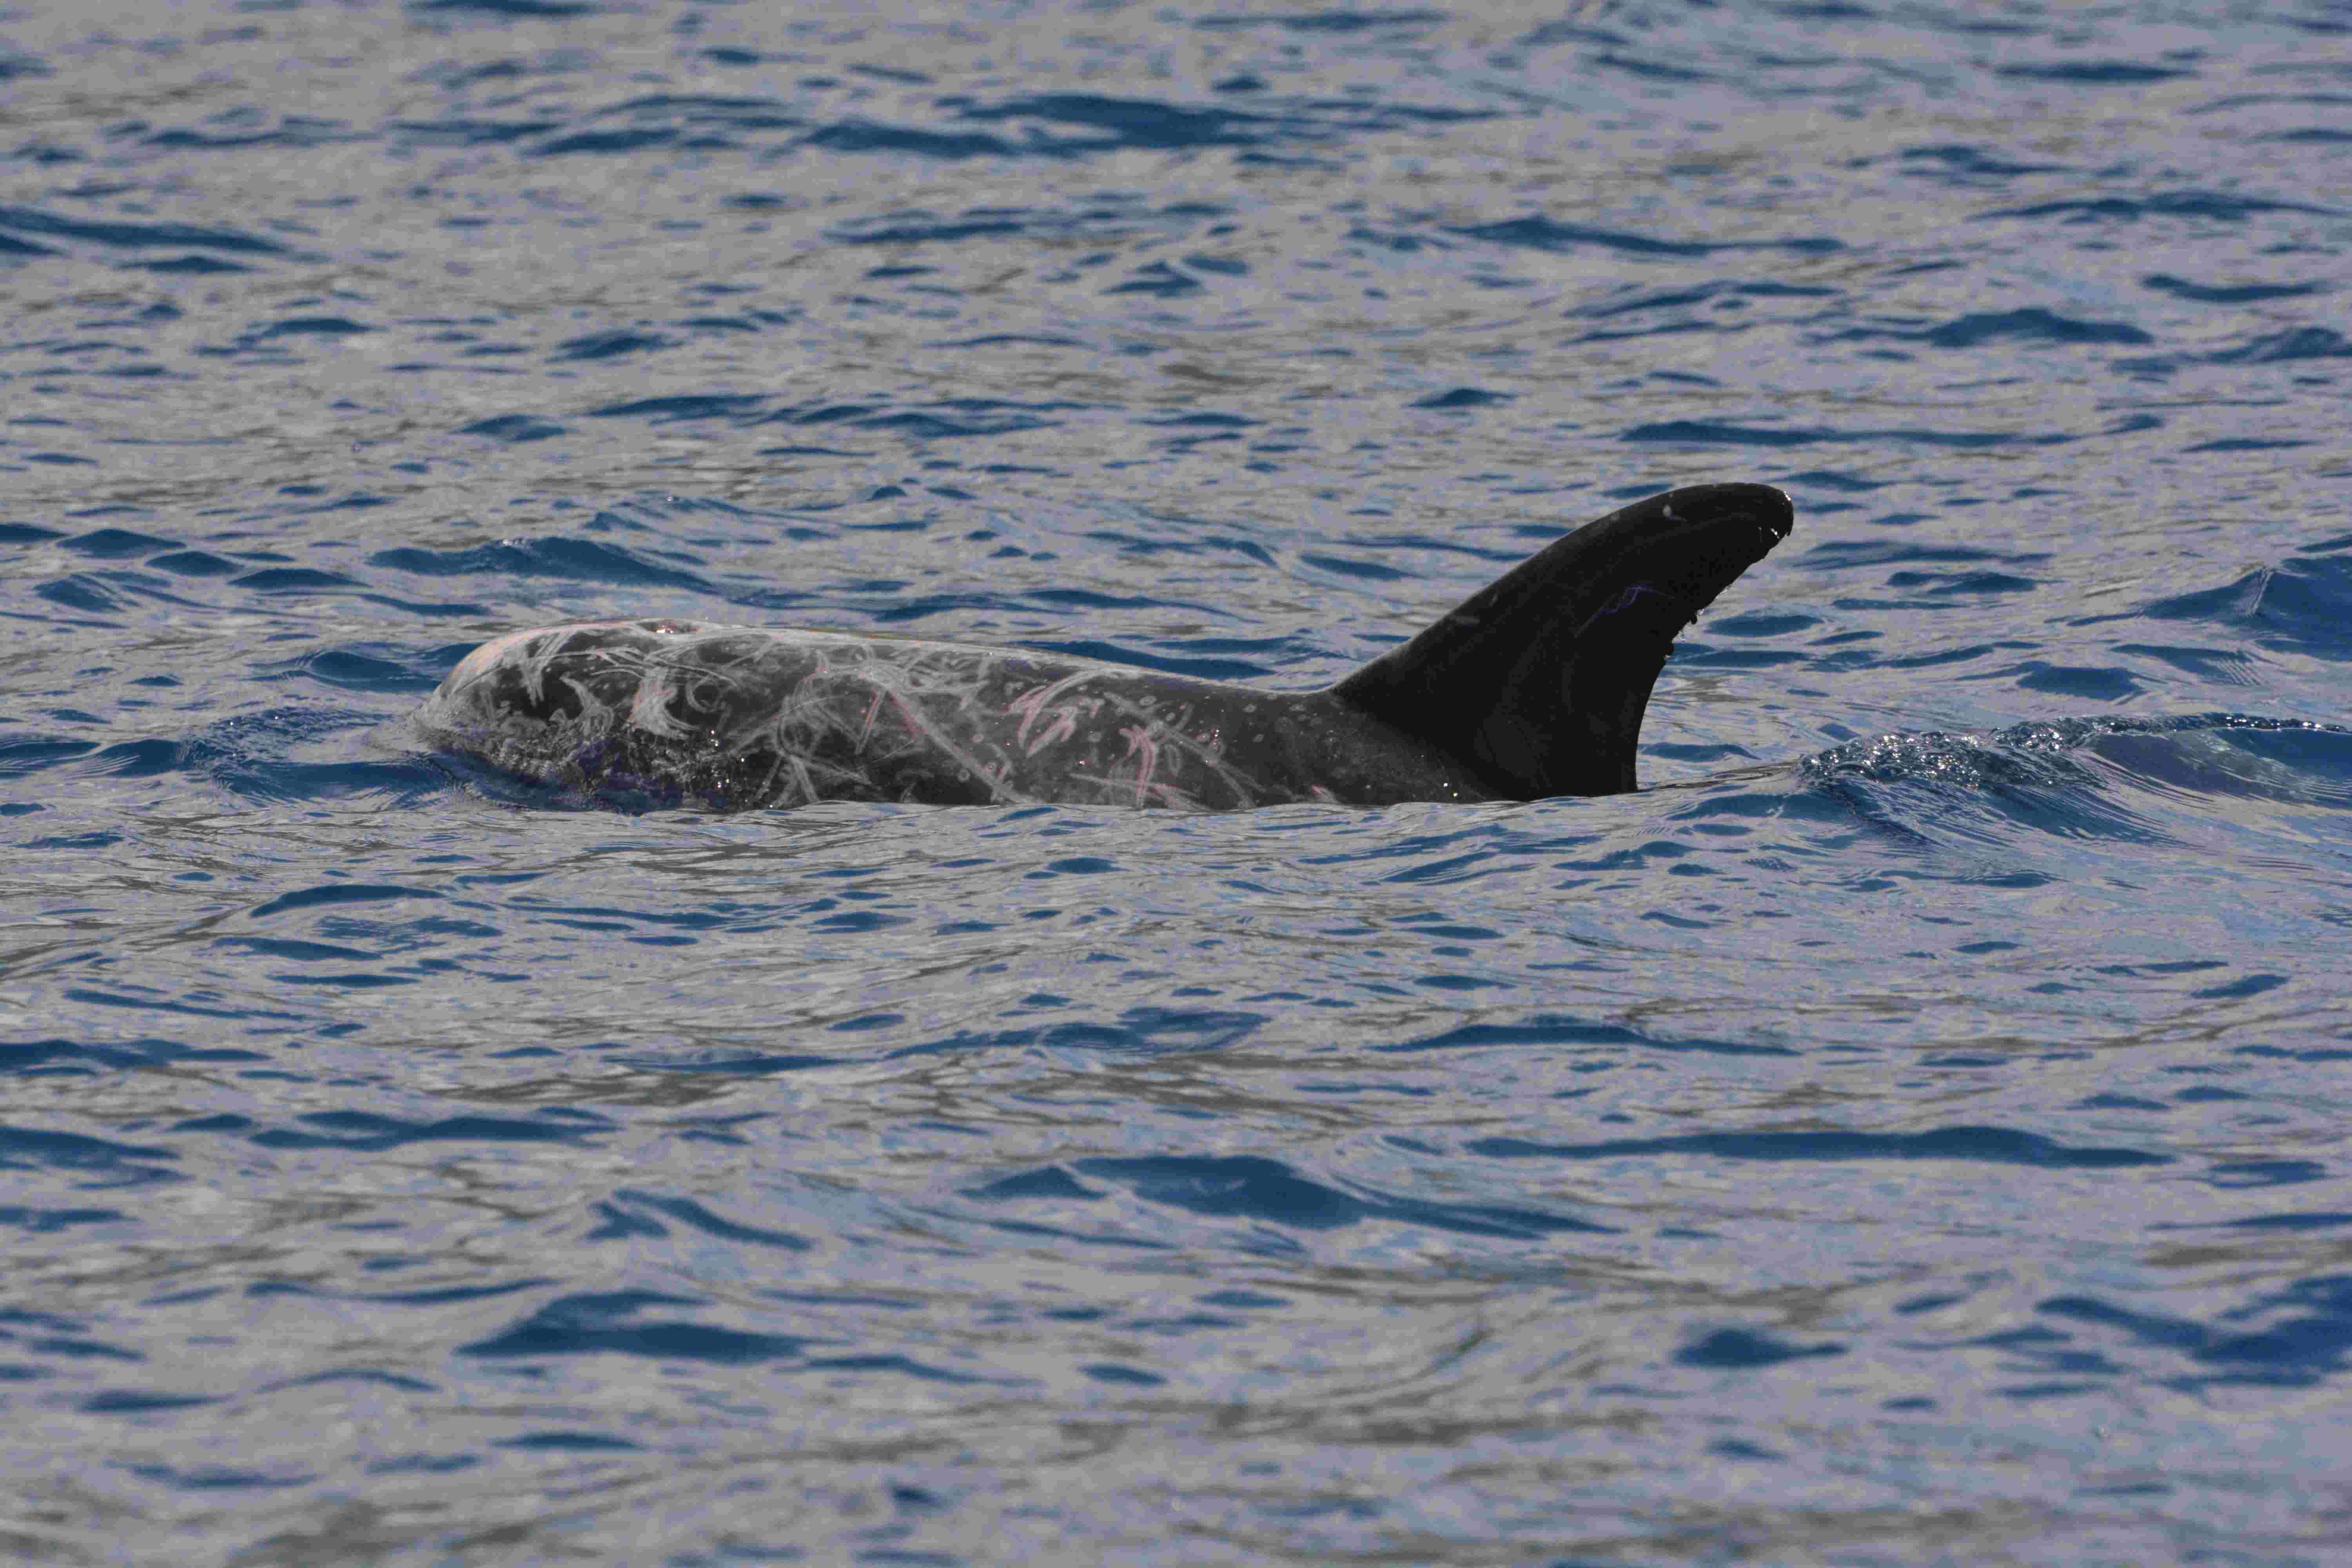
\includegraphics[width=0.24\textwidth]{a1.jpg}
    \hfill
    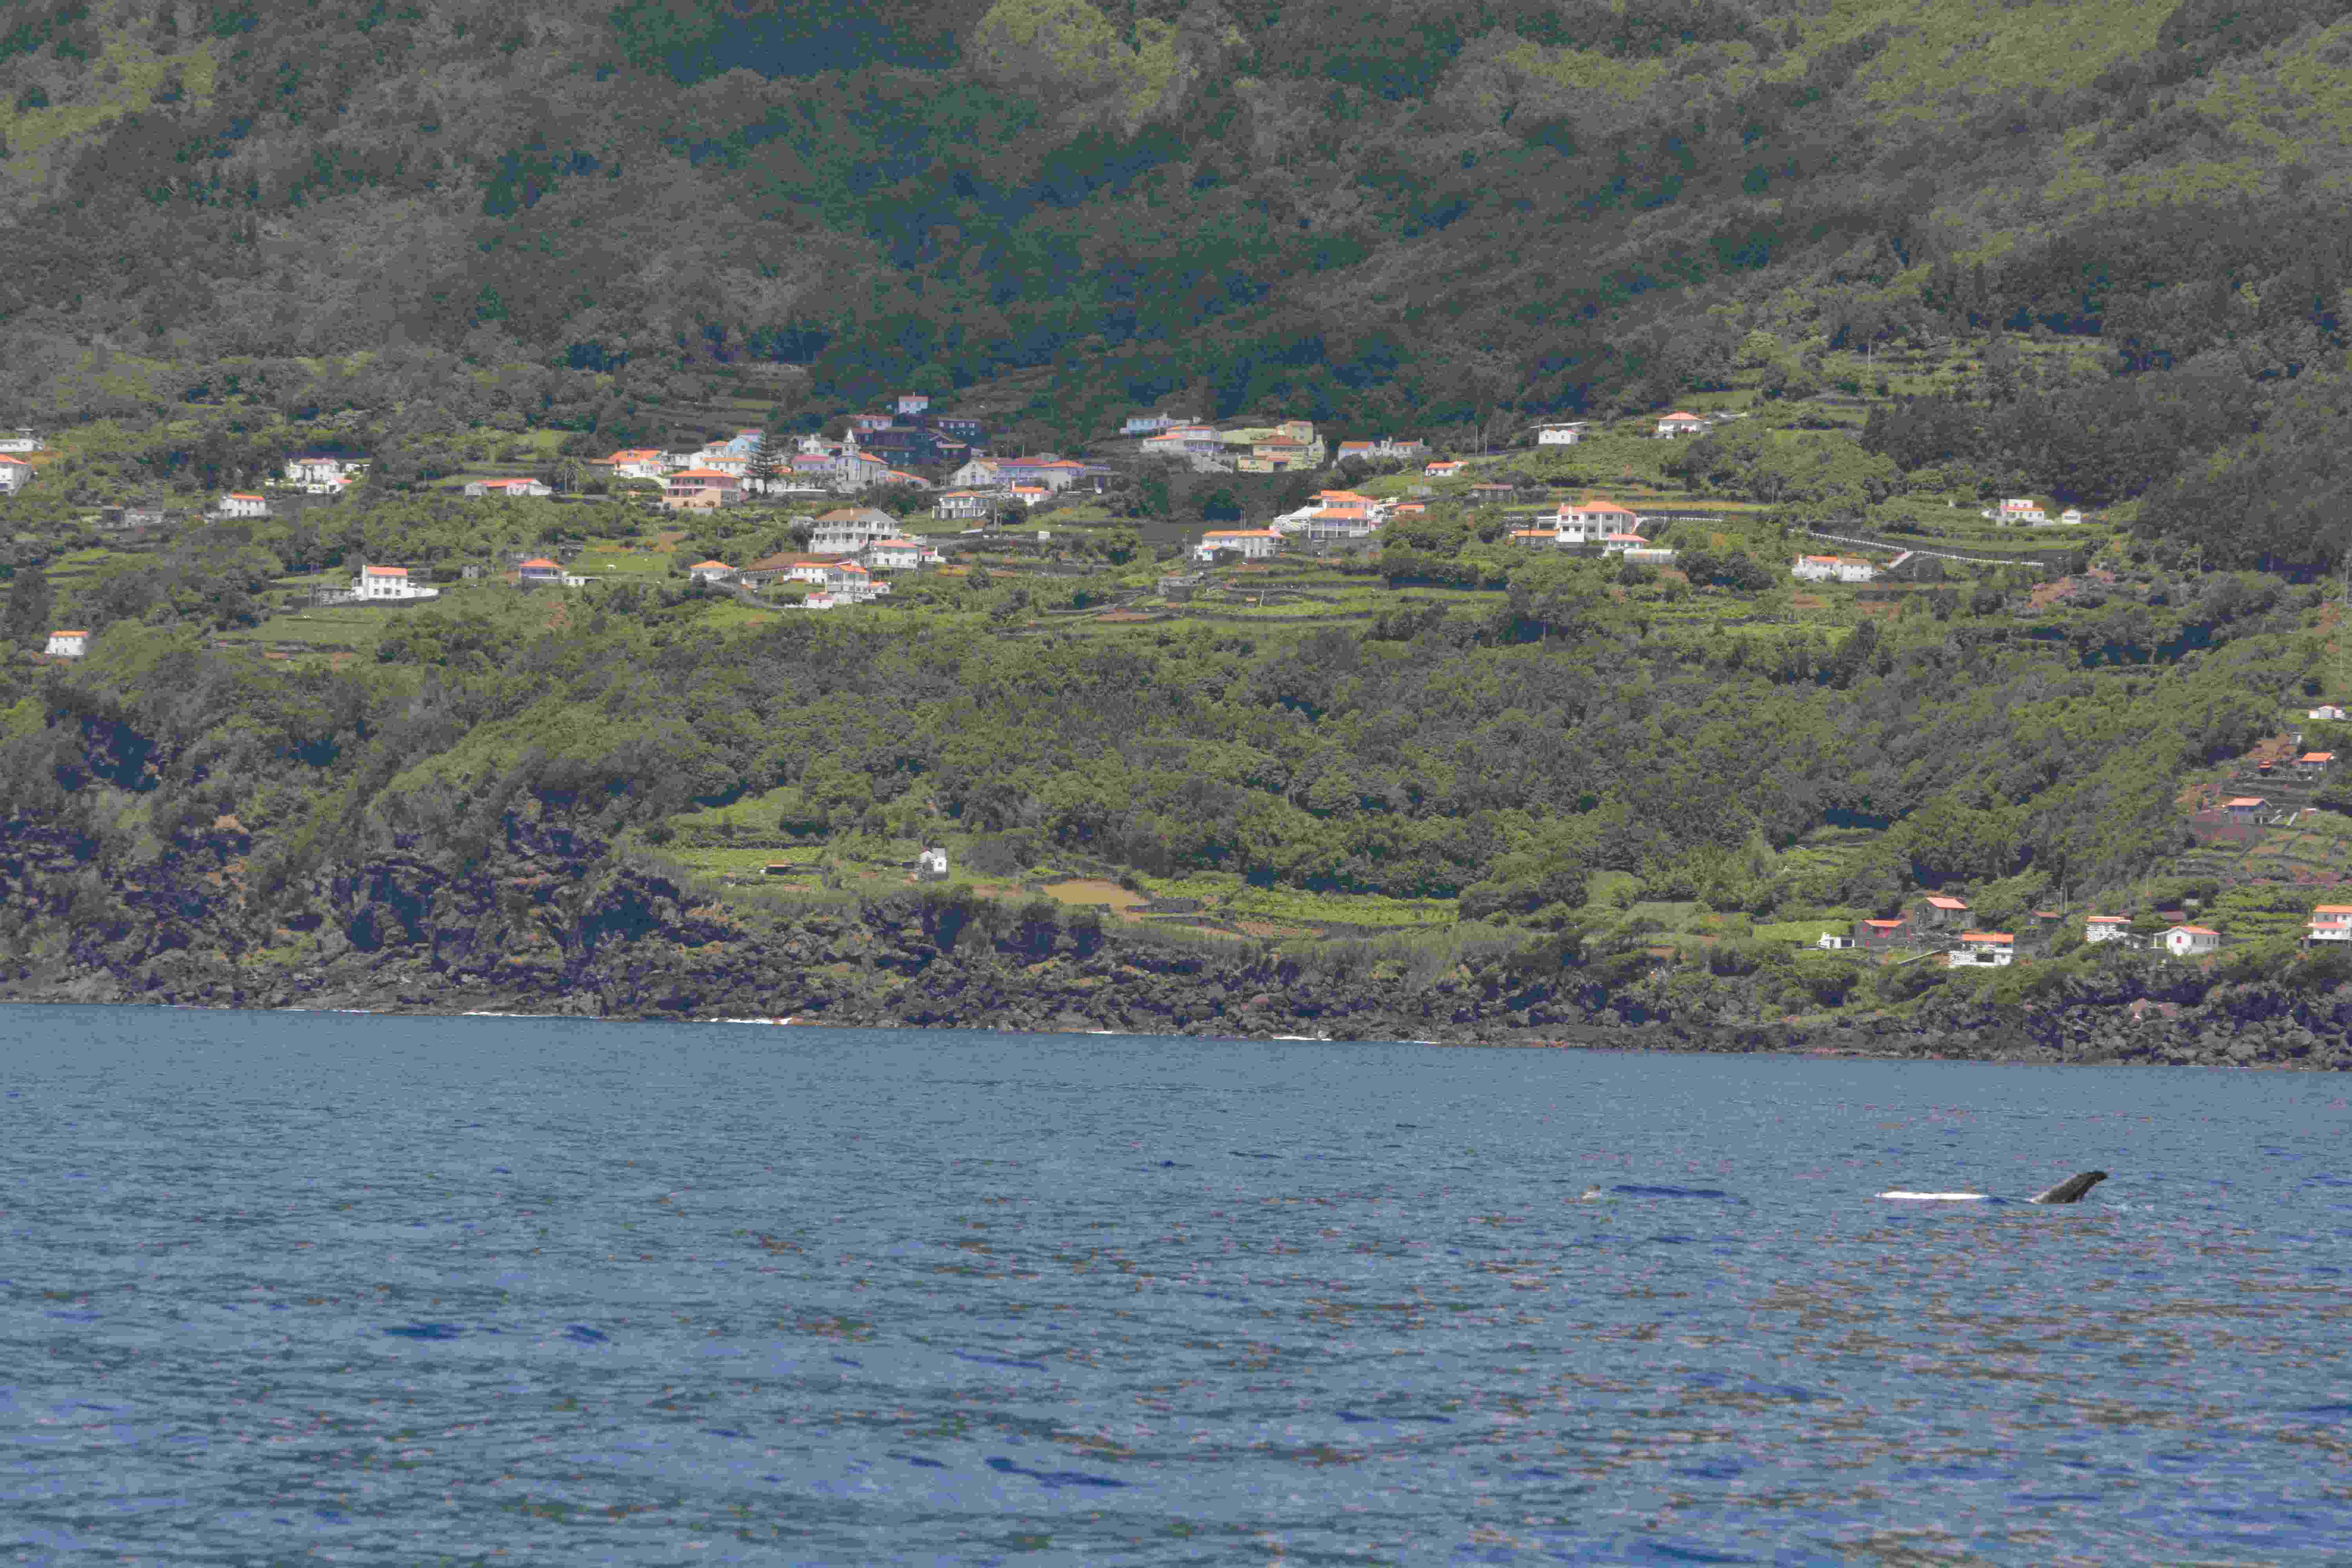
\includegraphics[width=0.24\linewidth]{a2.jpg}
    \hfill
    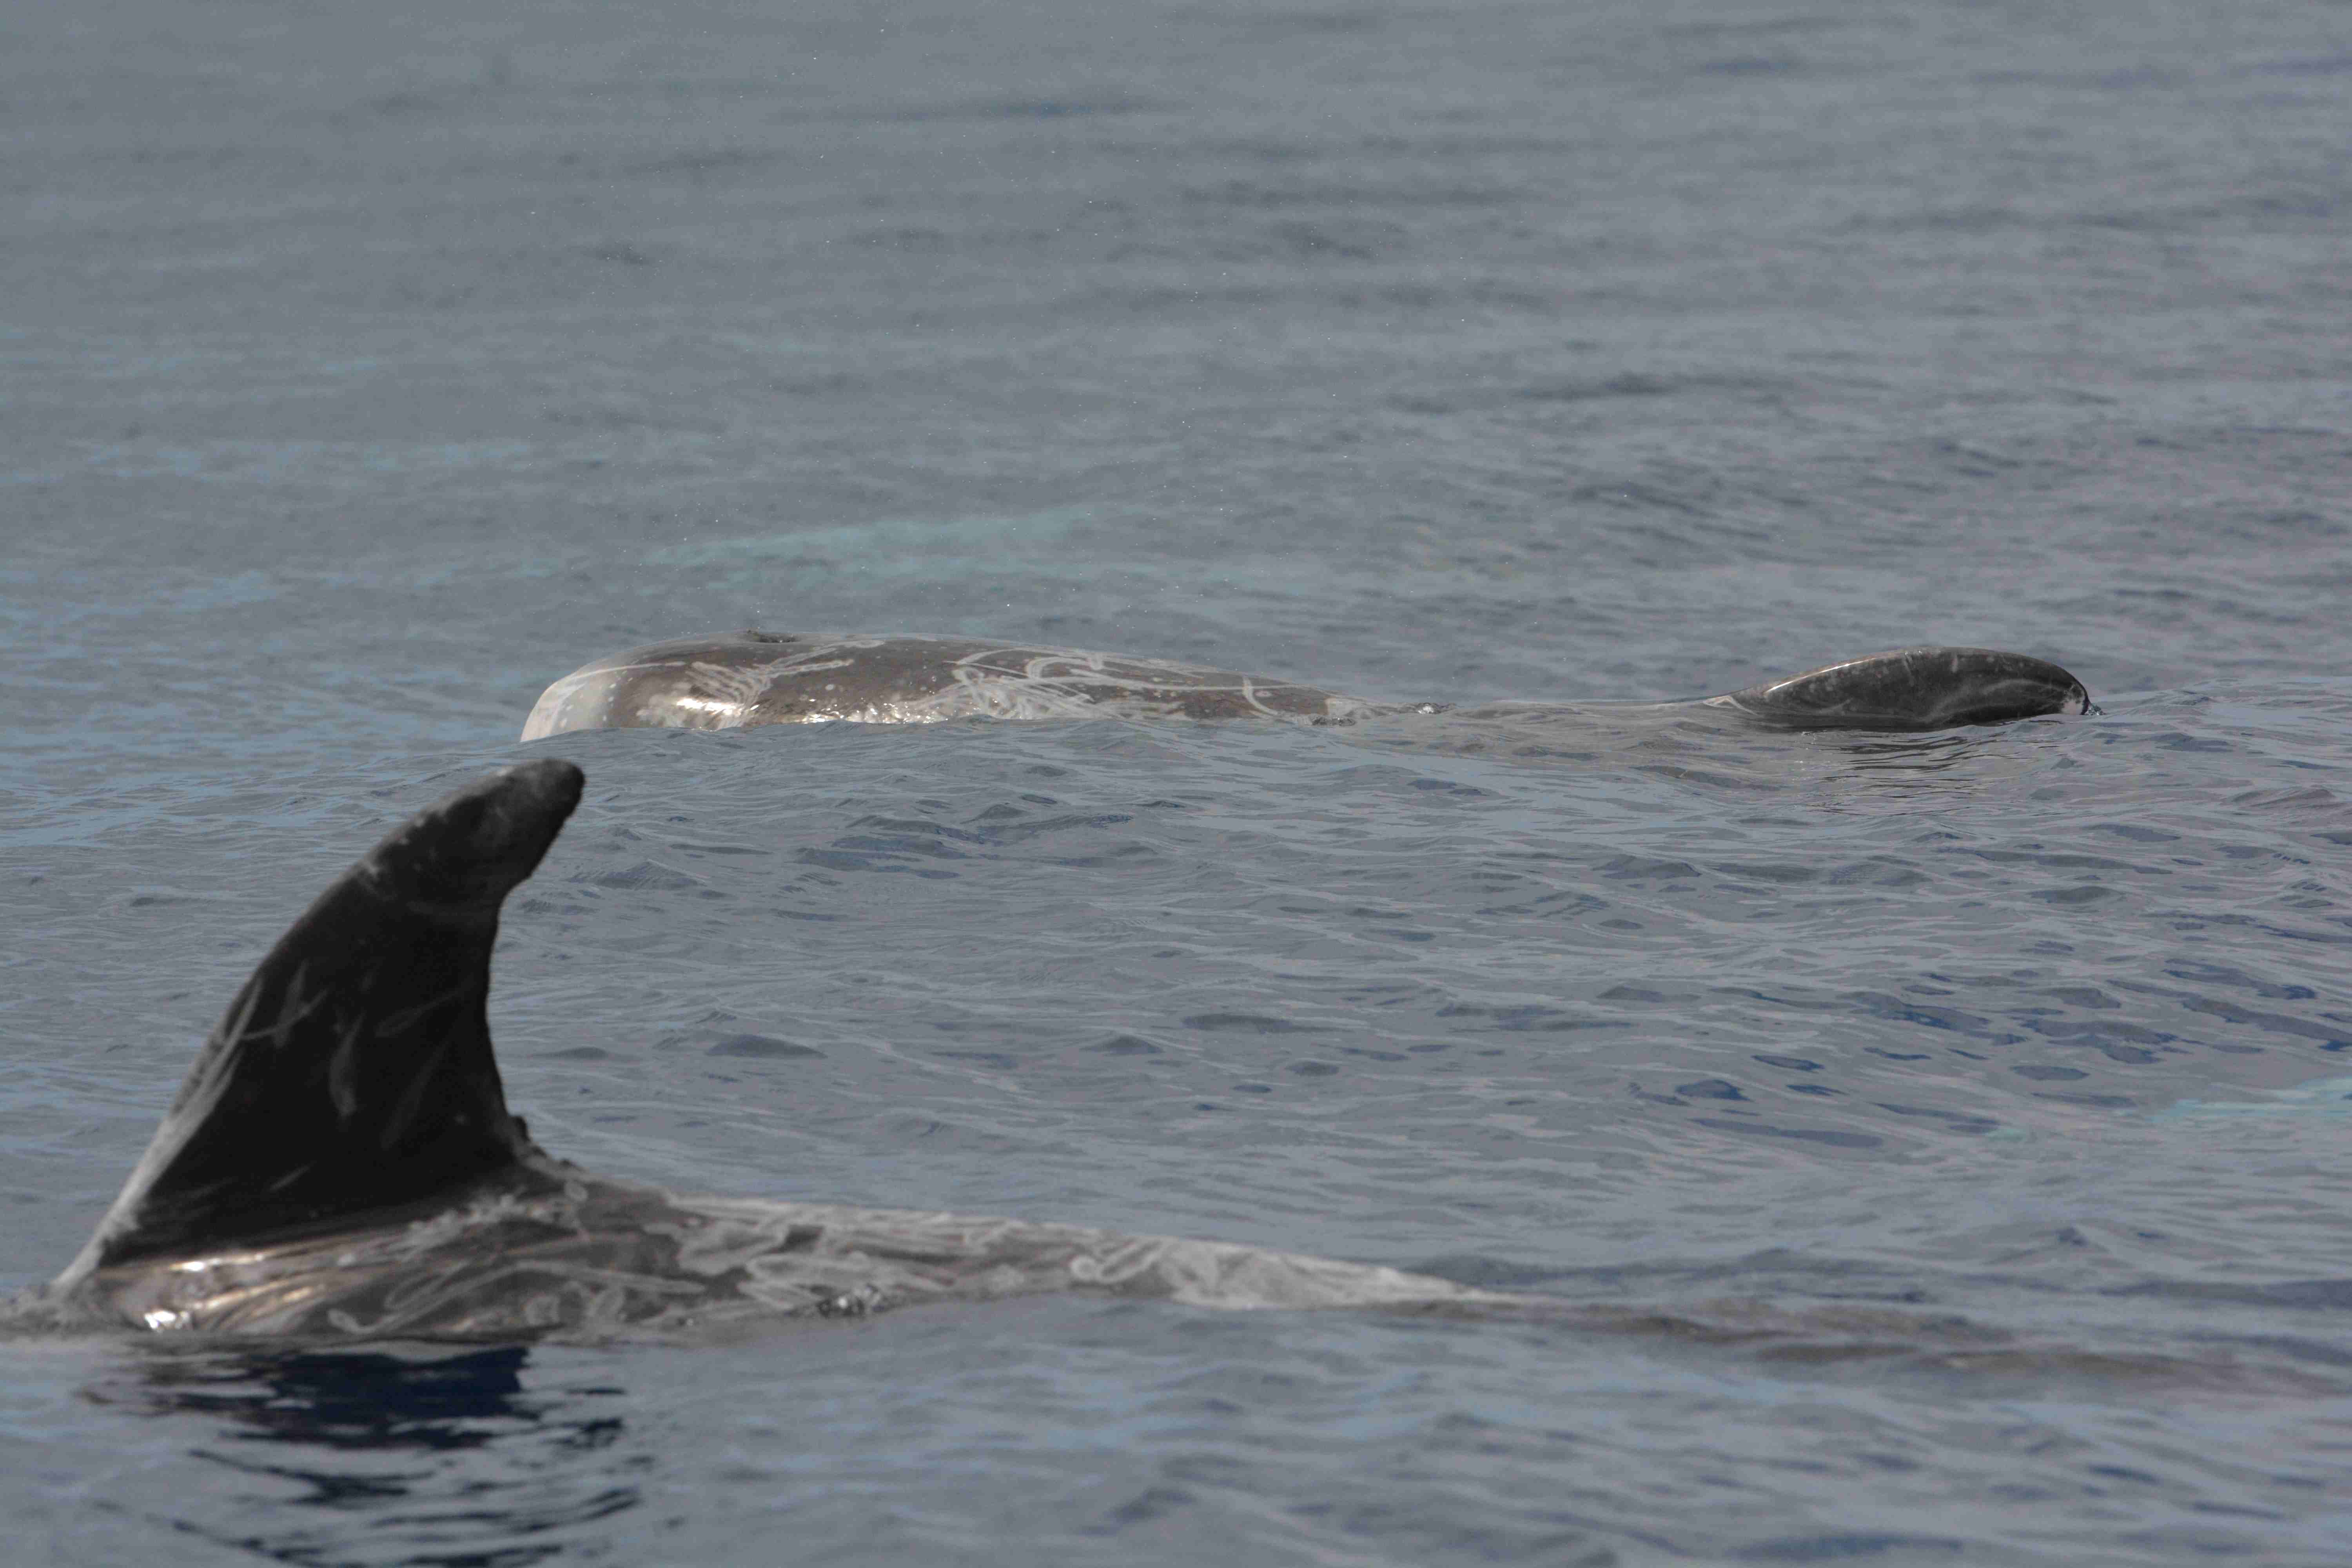
\includegraphics[width=0.24\linewidth]{a3.jpg}
    \hfill
    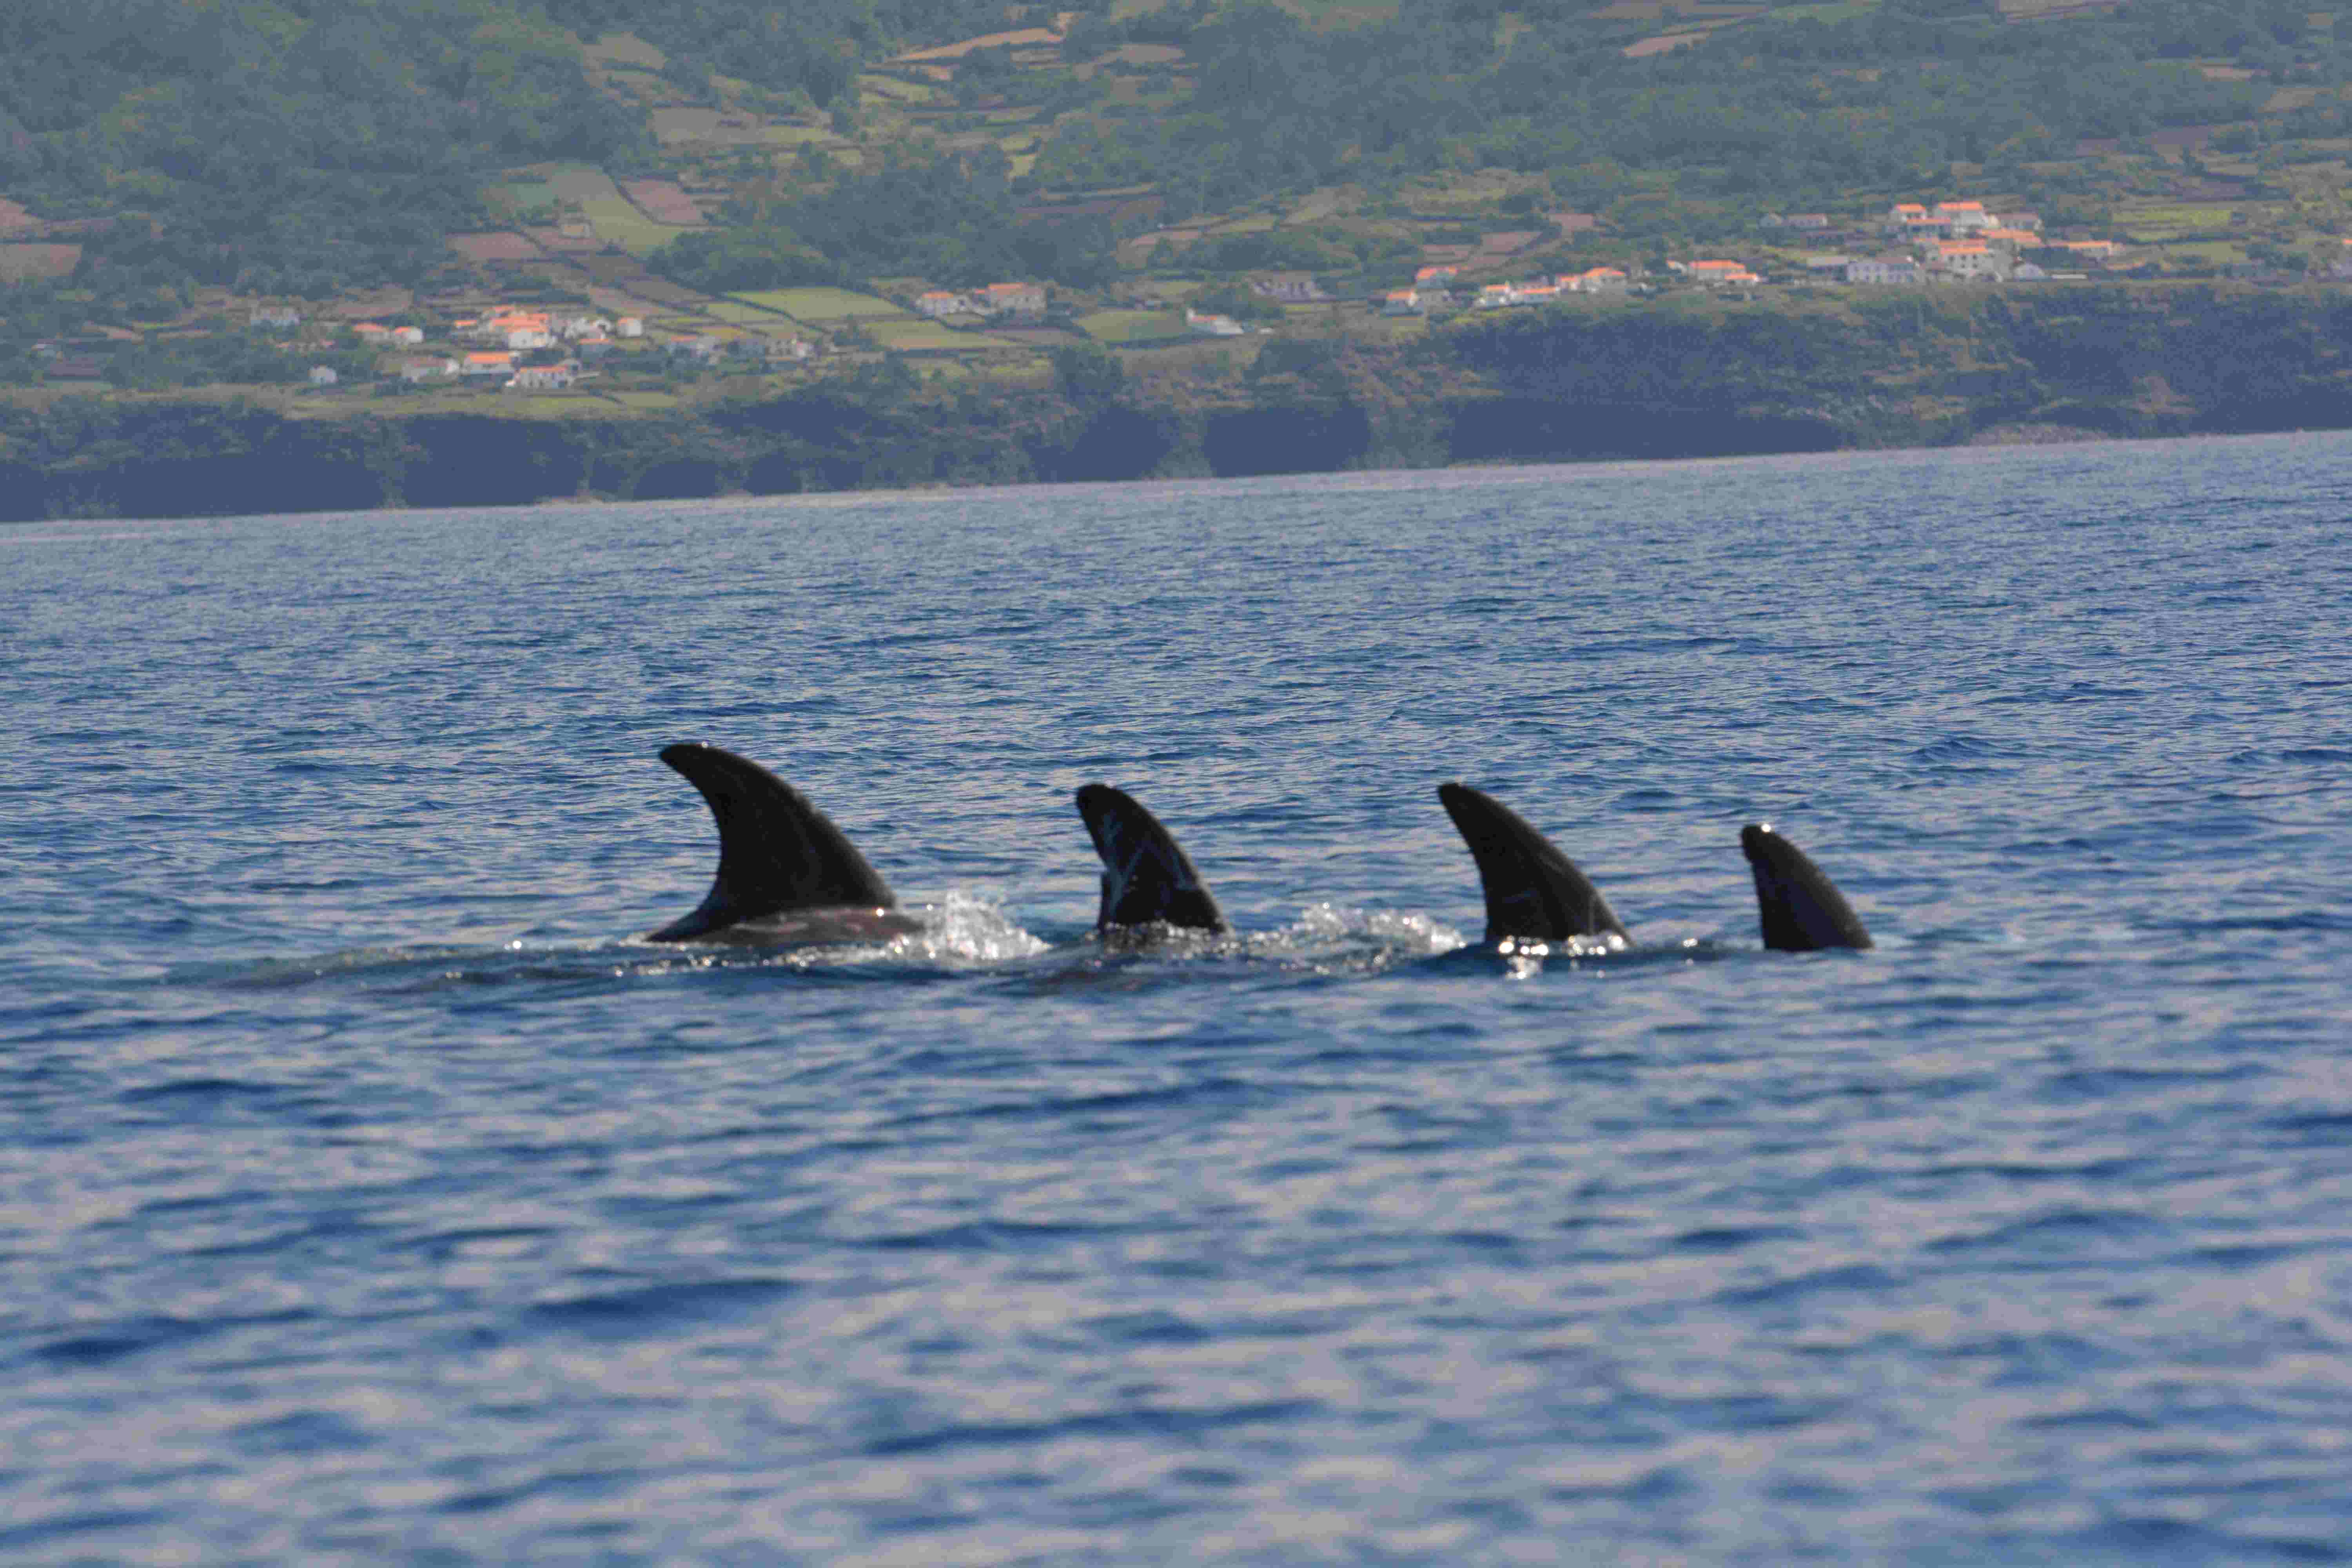
\includegraphics[width=0.24\linewidth]{a4.jpg}
    \caption{}
  \end{subfigure}
  
  \caption{Alcune immagini estrapolate dai due dataset utilizzati. (a) Dataset degli scatti di Taranto, (b) Dataset degli scatti delle Azzorre. Si noti la presenza di foto con disturbi o addirittura senza alcun valore informativo ai fini dello studio dei cetacei.}
  \label{fig:esempiDataset}
\end{figure}

Si rende perciò necessario filtrare in qualche modo le sole immagini che raffigurano al loro interno pinne dorsali di cetacei; è utile inoltre ritagliare da queste immagini filtrate le sole regioni in cui è effettivamente presente una pinna (si vuole cioè isolare l'informazione utile dal resto del dato originale). Per far questo, i due dataset sono stati rielaborati attraverso un \textbf{algoritmo di riconoscimento e cropping} delle pinne dorsali, di seguito descritto nelle sue caratteristiche salienti.

\section{CropFin v1}
\label{cropFin}
Per ritagliare ed estrarre dalle immagini originali le sole pinne dorsali, è stata utilizzata la routine \textit{CropFin v1} in linguaggio MATLAB sviluppata in \cite{gianvito} sulla base di un precedente lavoro  \cite{flavio}.
Si può descrivere la routine in due fasi:
\begin{enumerate}
\item Segmentazione, filtraggio e ritaglio adattivo delle regioni delle immagini che possono verosimilmente contenere una pinna
\item Classificazione di ogni ritaglio ottenuto in due classi 'Pinna' e 'No Pinna', mediante una rete neurale artificiale creata \textit{ad-hoc}.
\end{enumerate}

La novità introdotta dal presente lavoro di tesi in merito al problema di estrazione delle pinne da un'immagine riguarda l'utilizzo di un metodo di classificazione basato sul \textit{transfer learning}. In pratica, quindi, la principale differenza rispetto a CropFin v1 è nella seconda fase della routine: la classificazione avviene con l'utilizzo non più di una rete artificiale creata da zero per il problema in analisi, bensì riutilizzando un insieme di reti neurali profonde addestrate su un diverso problema di classificazione e adattate al nostro task. Questo nuovo modello è descritto dettagliatamente nel par. \ref{esperimentoTL}.\\

Al fine di ottenere i ritagli delle pinne, la routine adoperata attua una sequenza di operazioni di preprocessing su ciascuna immagine per poi individuare ed infine ritagliare e salvare separatamente le sole porzioni di immagini che possono eventualmente contenere pinne. Tale sequenza è implementata mediante un ciclo \verb|for| che cicla su ogni immagine del dataset. Di seguito sono descritte sinteticamente le operazioni, nell'ordine in cui vengono applicate. Le figure esplicative per ogni fase provengono dalla tesi triennale dell'ing. Losapio \cite{gianvito}, a cui vanno i crediti.

\subsection{Fase di ritaglio}
\label{faseRitaglio}

\subsection*{Ridimensionamento}
L'immagine è innanzitutto ridimensionata mediante la funzione MATLAB \verb|imresize| con un fattore di scale $\times 0.2$, al fine di ottenere una nuova immagine di risoluzione più bassa ($1200\times 800$).
Questa operazione di preprocessing è stata adottata per diminuire il costo computazionale delle operazioni successive.\footnote{La risoluzione di partenza delle immagini utilizzate è stata $6000\times 4000$, ottenendo una riduzione drastica di pixel del 96\%, da 24 milioni a 960 mila.}\\

\noindent Il risultato dell'operazione è visualizzato in figura \ref{fig:ridimensionamento}

\begin{figure}[h]
  \centering
  \begin{subfigure}[b]{0.475\textwidth}
    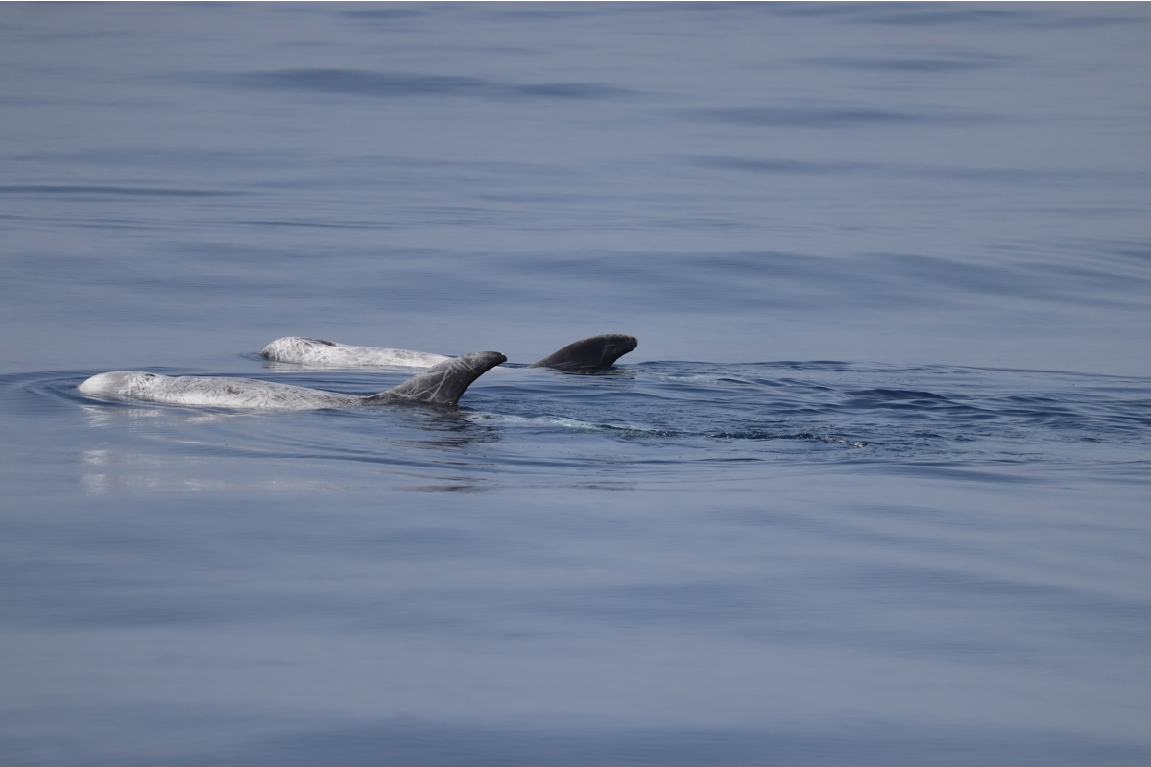
\includegraphics[width=\textwidth]{immagineDaProcessare.png}
    \caption{Prima del ridimensionamento}
  \end{subfigure}
  \begin{subfigure}[b]{0.475\textwidth}
  \centering
    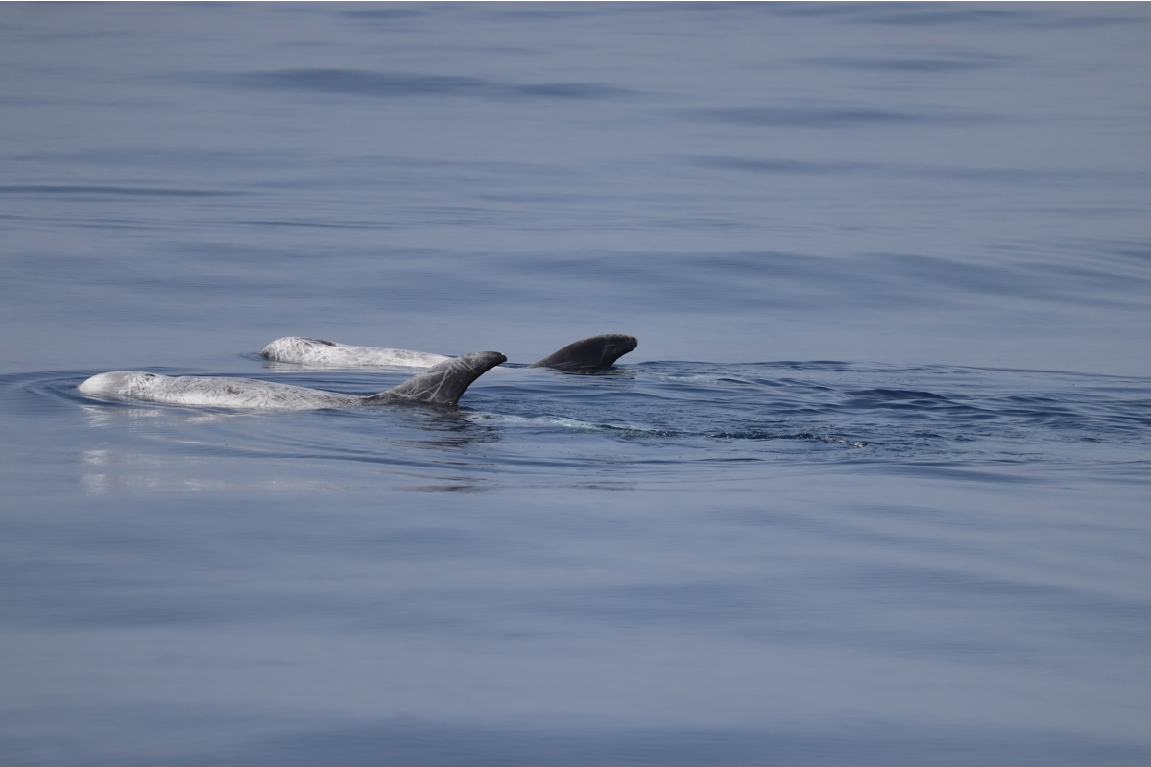
\includegraphics[width=0.2\textwidth]{immagineDaProcessare.png}
    \caption{Dopo il ridimensionamento}
  \end{subfigure}
  \caption{Ridimensionamento di un'immagine (scelta nel dataset degli scatti di Taranto)}
  \label{fig:ridimensionamento}
\end{figure}


\subsection*{CLAHE}
L'immagine ridimensionata è sottoposta ad una equalizzazione adattiva dell’istogramma a contrasto limitato (CLAHE). Questa operazione consente un miglioramento del contrasto dell'immagine, proprietà utile per migliorare l'efficienza della successiva operazione, la sogliatura dell'immagine secondo il metodo di Otsu.\\

\noindent Il risultato dell'operazione è visualizzato in figura \ref{fig:clahe}

\begin{figure}[h]

  \centering
  
  \begin{subfigure}[b]{0.42\textwidth}
    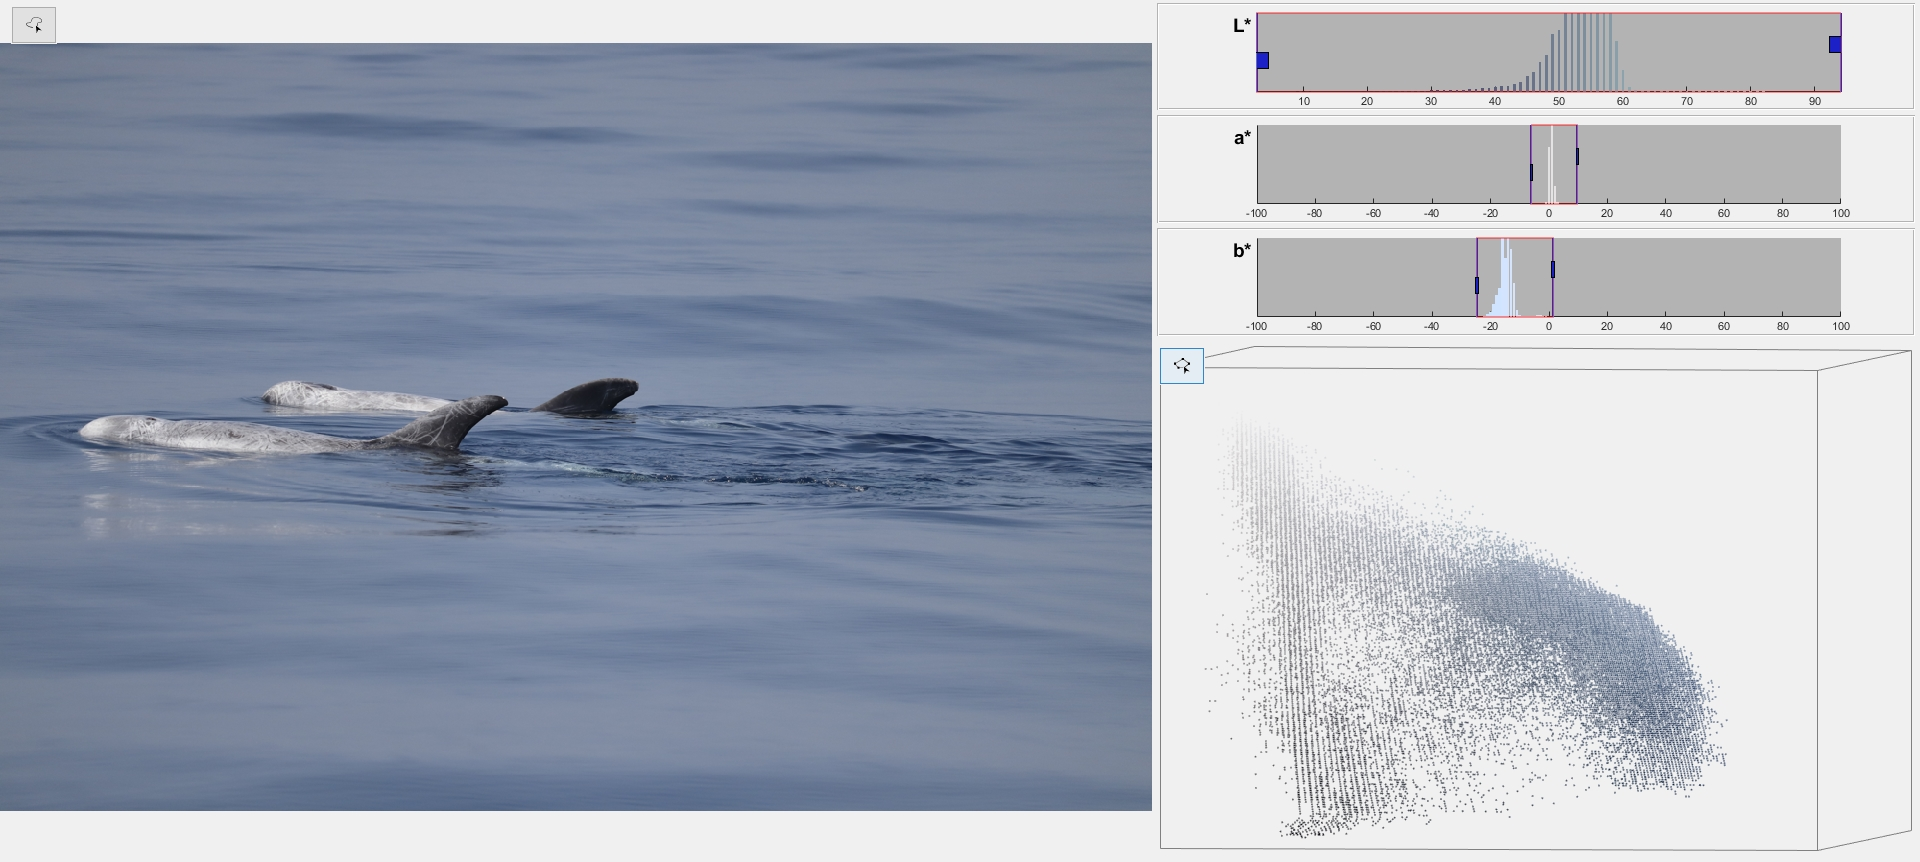
\includegraphics[width=\textwidth]{primaClahe.jpg}
    \caption{Prima dell'applicazione di CLAHE}
  \end{subfigure}
  \begin{subfigure}[b]{0.42\textwidth}
  \centering
    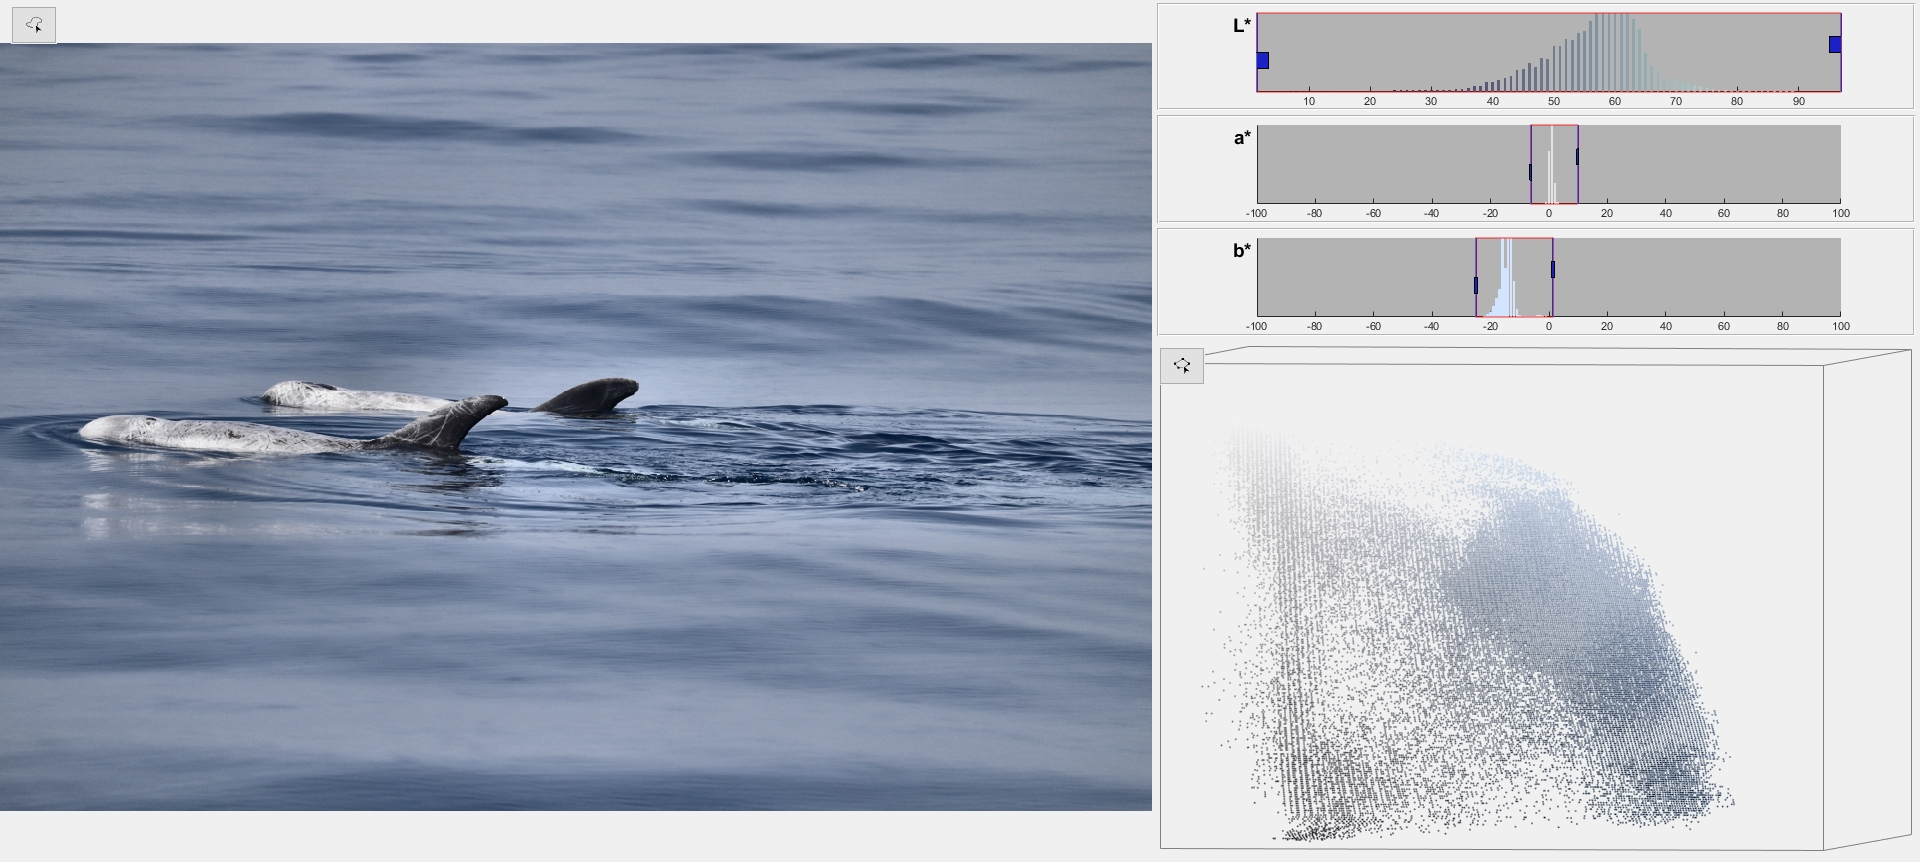
\includegraphics[width=\textwidth]{dopoClahe.jpg}
    \caption{Dopo l'applicazione di CLAHE}
  \end{subfigure}
  
  \caption{Applicazione dell'equalizzazione CLAHE all'immagine, con visualizzazione dell'istogramma nello spazio dei colori \textit{L*a*b*}. NB: per semplicità l'immagine è raffigurata riportandola alle sue dimensioni originali}
  \label{fig:clahe}
\end{figure}

\subsection*{Segmentazione}
L'immagine viene segmentata (cioè ogni pixel viene assegnato ad una di due classi: \textit{background} e \textit{foreground}) mediante il metodo di Otsu per la sogliatura automatica \cite{otsu}.

Il metodo di Otsu viene usato nella sua versione classica a due livelli, rispetto agli istogrammi dei canali L e b. In particolare, viene applicata la sogliatura secondo Otsu separatamente al canale L e b, cioè calcolate le soglie di Otsu per i due canali, mediante la funzione \verb|multithresh|.
Avendo a disposizione tali soglie, l’ipotesi avanzata è che le pinne dorsali possano essere
isolate considerando le regioni di immagine che siano contemporaneamente:
\begin{itemize}
\item nella regione più scura del canale L, cioè a sinistra della soglia sul canale L
\item nella regione contenente il grigio del canale b, cioè a destra della soglia sul canale b
\end{itemize}
L'immagine segmentata (binarizzata) finale è ottenuta quindi annerendo quei pixel dell'immagine che non verificano le seguenti condizioni (o, equivalentemente, rendendo bianchi i pixel che le verificano)\footnote{L’idea alla base di questo approccio nasce da una precisa conoscenza del dominio e da alcune ipotesi a priori riguardanti il contenuto delle immagini. In particolare, si suppone
che esse contengano generalmente solo mare (background) e cetacei (foreground),
e che queste due classi di oggetti contribuiscano alla creazione di due aree distinte e
separabili degli istogrammi dei canali L e b. Volendo dare un’interpretazione intuitiva,
si tratta di separare ciò che è grigio e più scuro da ciò che è blu e più chiaro. La scelta
dello spazio di colori Lab è motivata proprio dalla possibilità di automatizzare questo
tipo intuitivo di segmentazione.}
\begin{itemize}
\item valore della componente L minore della soglia di Otsu sul canale L
\item valore della componente b maggiore della soglia di Otsu sul canale b
\end{itemize}

\noindent Il risultato dell'operazione è visualizzato in figura \ref{fig:otsu1}

\begin{figure}[h!]

  \centering
  
  \begin{subfigure}[b]{0.4\textwidth}
    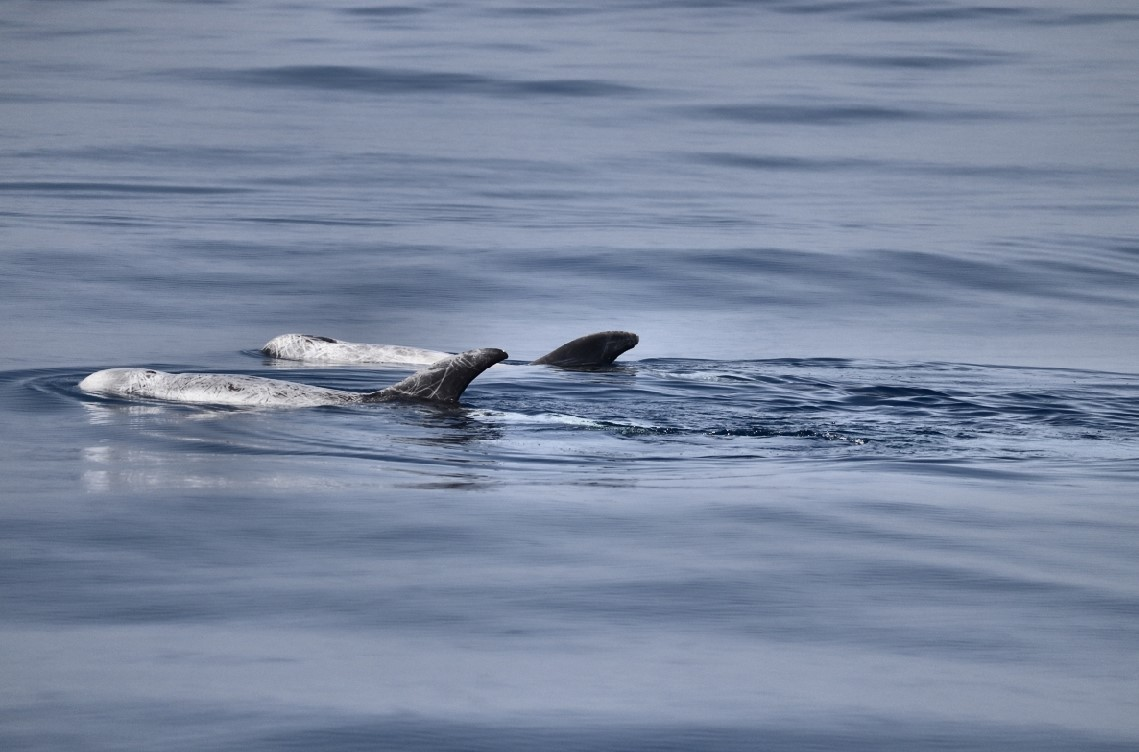
\includegraphics[width=0.95\textwidth]{primaOtsu.jpg}
    \caption{Prima della segmentazione secondo Otsu}
  \end{subfigure}
  \begin{subfigure}[b]{0.4\textwidth}
    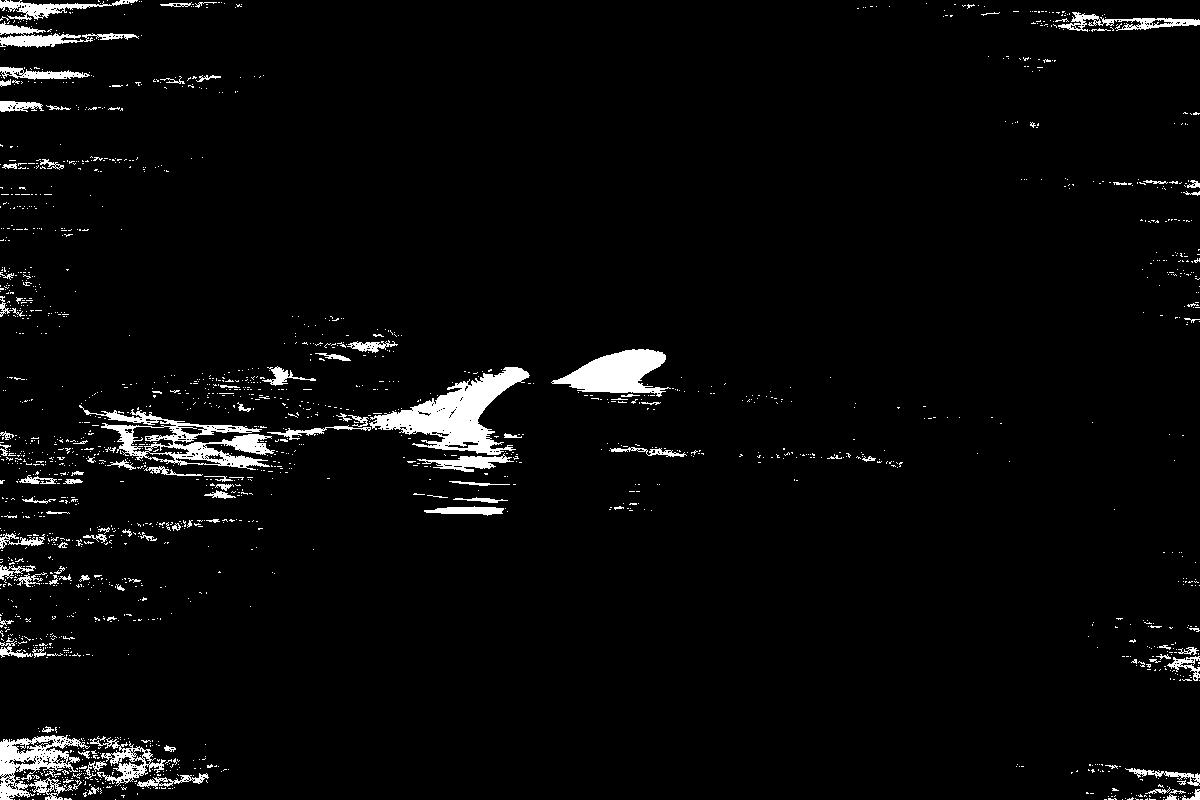
\includegraphics[width=0.95\textwidth]{dopoOtsu.jpg}
    \caption{Dopo la segmentazione secondo Otsu}
  \end{subfigure}
  
  \vspace{5mm}
  
  \begin{subfigure}[b]{0.5\textwidth}
  \centering
    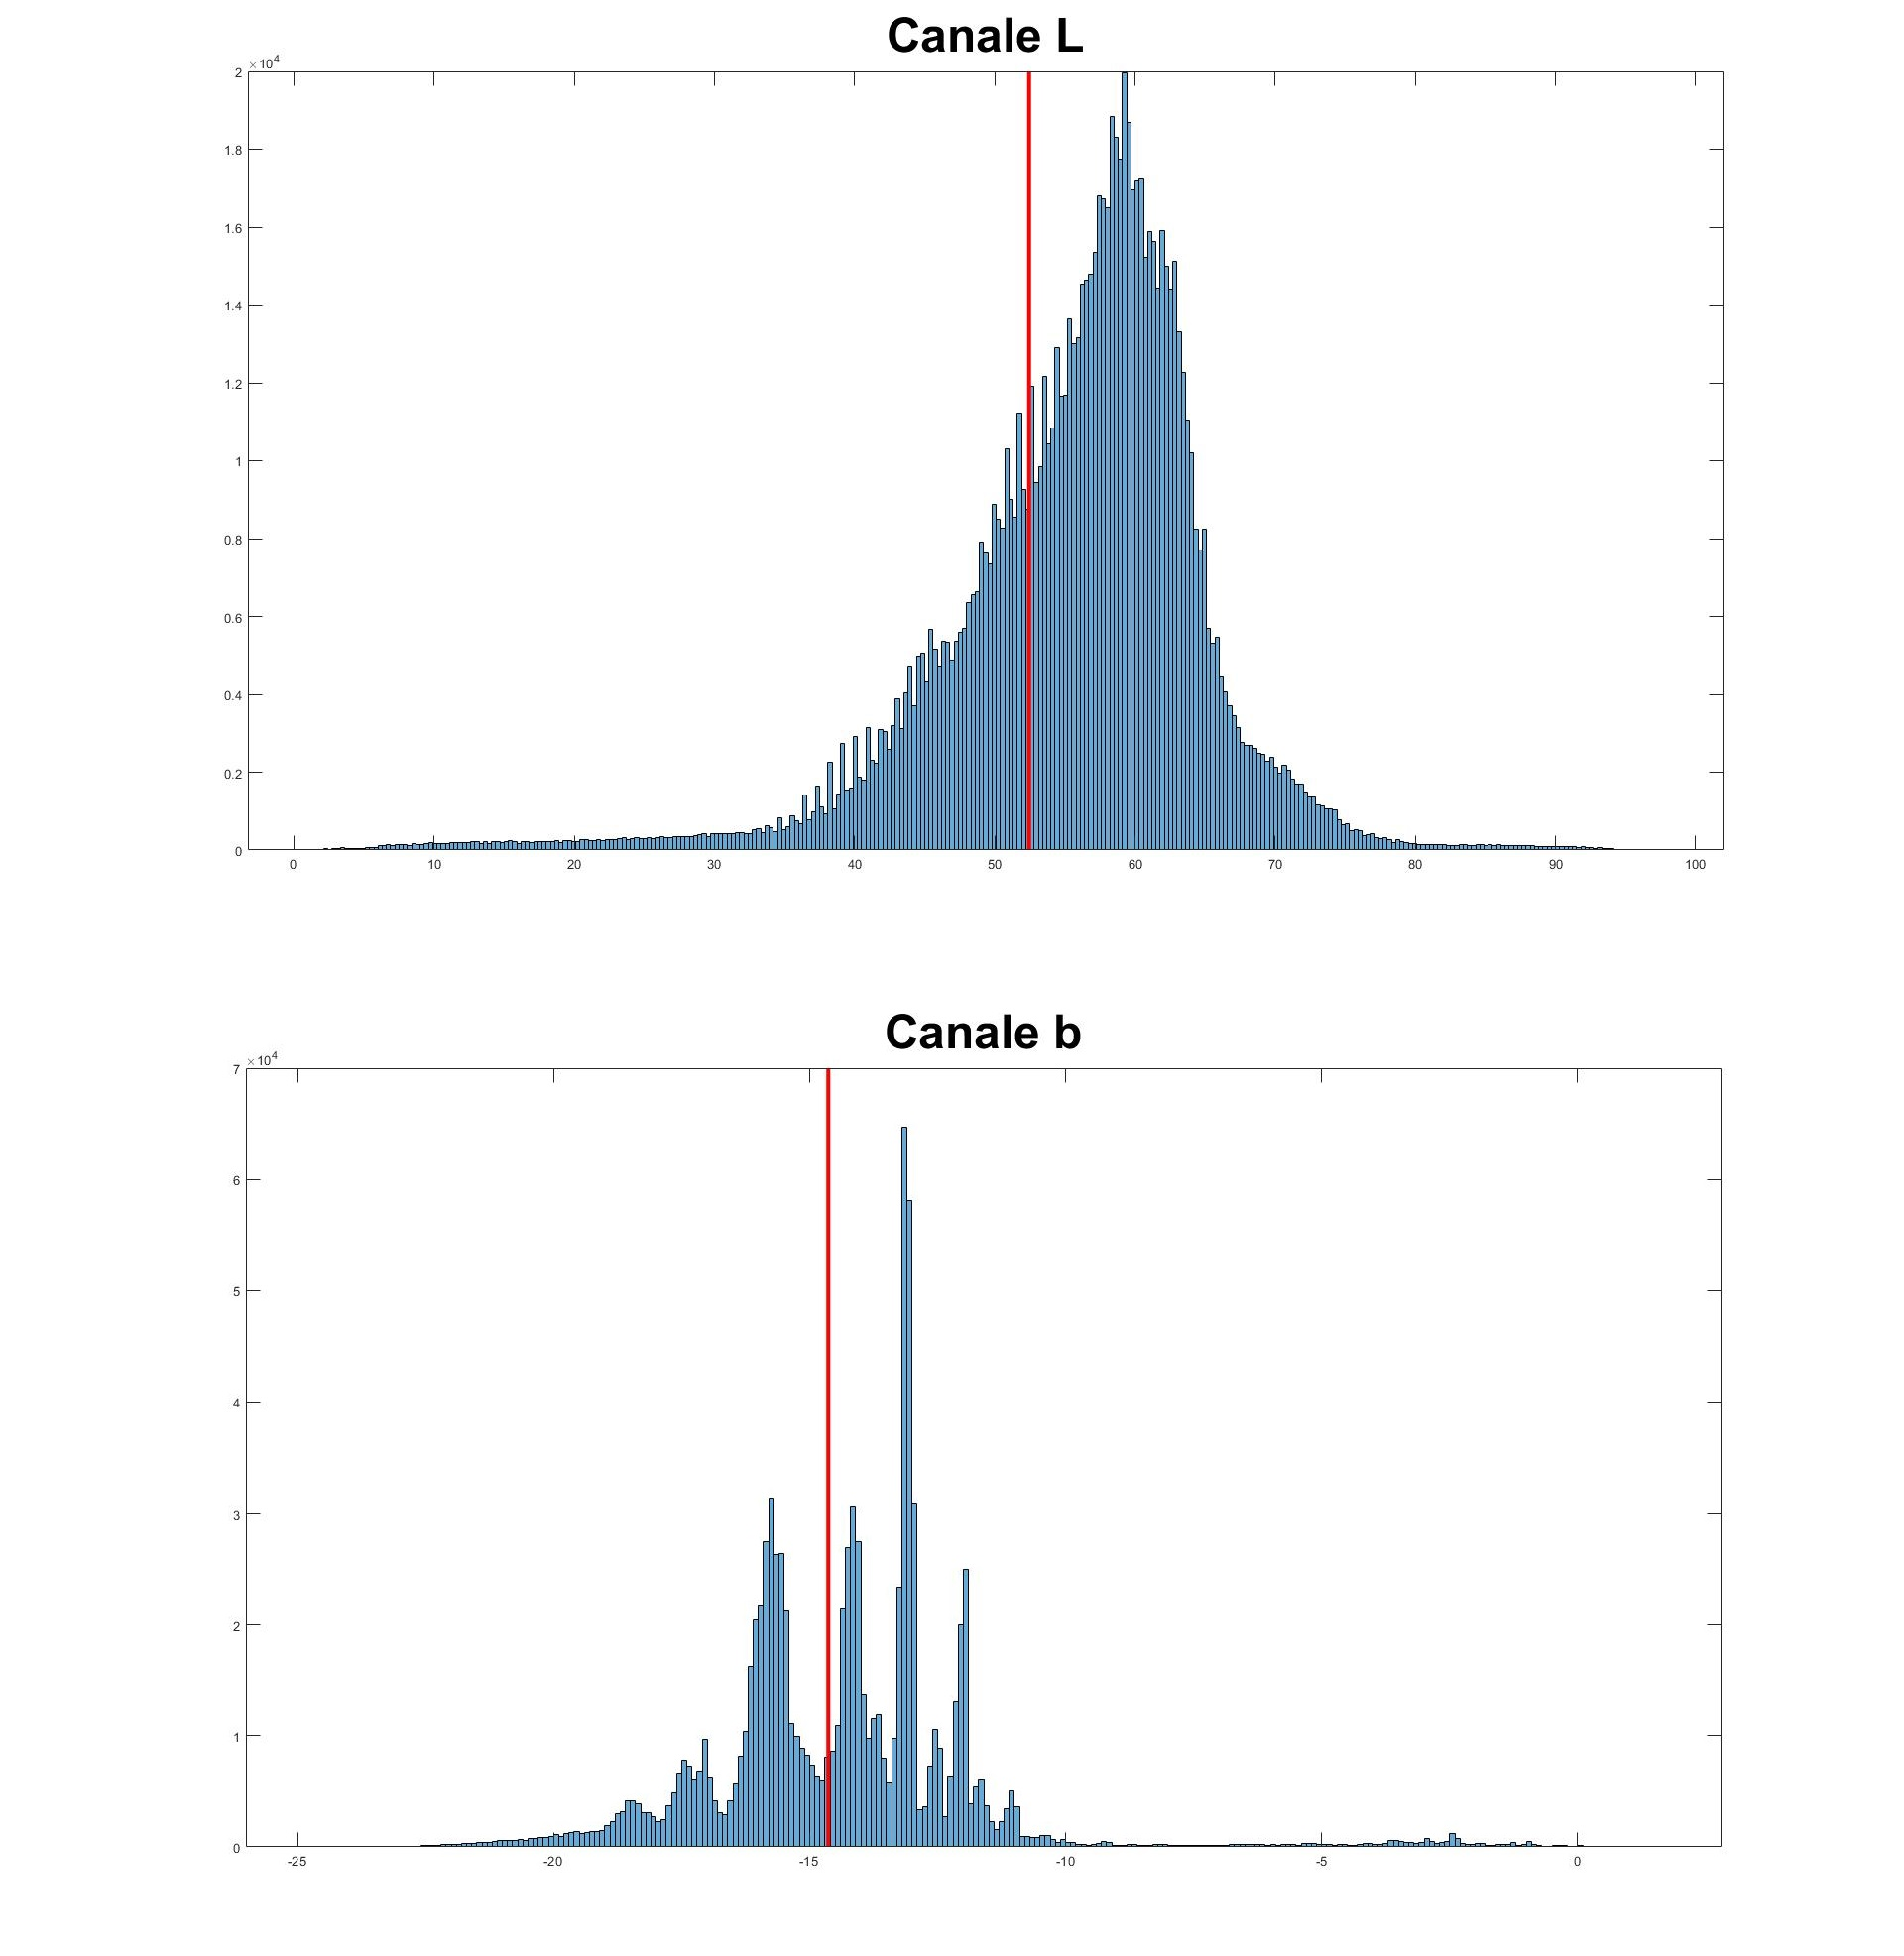
\includegraphics[width=\textwidth]{otsu.jpg}
    \caption{Individuazione delle soglie di Otsu per i canali L e b sui relativi istogrammi}
  \end{subfigure}
  
  \caption{Applicazione della segmentazione secondo Otsu nello spazio dei colori \textit{L*a*b*}}
  \label{fig:otsu1}
\end{figure}

\subsection*{Filtraggio delle regioni connesse}
L’immagine binaria ottenuta in seguito alla segmentazione viene filtrata in modo che siano scartate quelle regioni binarie connesse (anche dette \textit{blob}) che non presentano caratteristiche tali da poter rappresentare, verosimilmente, una pinna dorsale.
In particolare vengono utilizzati, consecutivamente due filtri:
\begin{enumerate}

\item il primo è applicato all'intera immagine binarizzata e serve a migliorare il risultato della sogliatura secondo Otsu.
Il filtro è configurato per mantenere, nell'ordine, le regioni connesse con le seguenti proprietà:
\begin{itemize}
\item prime 15 in ordine decrescente di \verb|Area| (n. di pixel che compongono la regione connessa)
\item \verb|Area| nel range \verb|[1600, 40000]|
\item \verb|Extent| nel range \verb|[-Inf, 0.55]| (rapporto tra \verb|Area| e il n. di pixel del più piccolo rettangolo che racchiude l'intera regione connessa, con i lati paralleli a due a due paralleli ai bordi dell'immagine)
\end{itemize}

\item il secondo è applicato come segue
\begin{enumerate}
\item Si ritaglia la foto originale in corrispondenza delle regioni mantenute in seguito all’applicazione del primo filtro, sulla base delle coordinate dei bounding box. Per ottenere ritagli leggermenti più larghi rispetto ai blob, al fine di non perdere eventuali parti della pinna erroneamente anneriti dopo la binarizzazione, ogni dimensione è aumentata del 20\%.
\item Si applica nuovamente, a ciascun ritaglio ottenuto, la sogliatura basata sul metodo di Otsu. In questo caso è omesso il miglioramento del contrasto mediante CLAHE prima del calcolo dei valori di soglia.
\item Si introduce a questo punto il secondo filtro, applicato alle regioni binarie ottenute per ciascun ritaglio. L’unico parametro utilizzato in questo caso è il seguente:
\begin{itemize}
\item \verb|Area| nel range \verb|[20000, 1000000]|
\end{itemize}
con lo scopo di isolare l’eventuale pinna (che rappresenta sicuramente la regione di area maggiore all’interno di ciascun ritaglio) in modo che possa essere sottoposta all’algoritmo di ritaglio adattivo, descritto nella sezione successiva.
\end{enumerate}
\end{enumerate}

\noindent Il risultato dell'operazione è visualizzato in figura \ref{fig:filtraggioBlob}

\begin{figure}[h!]

  \centering
  
  \begin{subfigure}[b]{0.8\textwidth}
    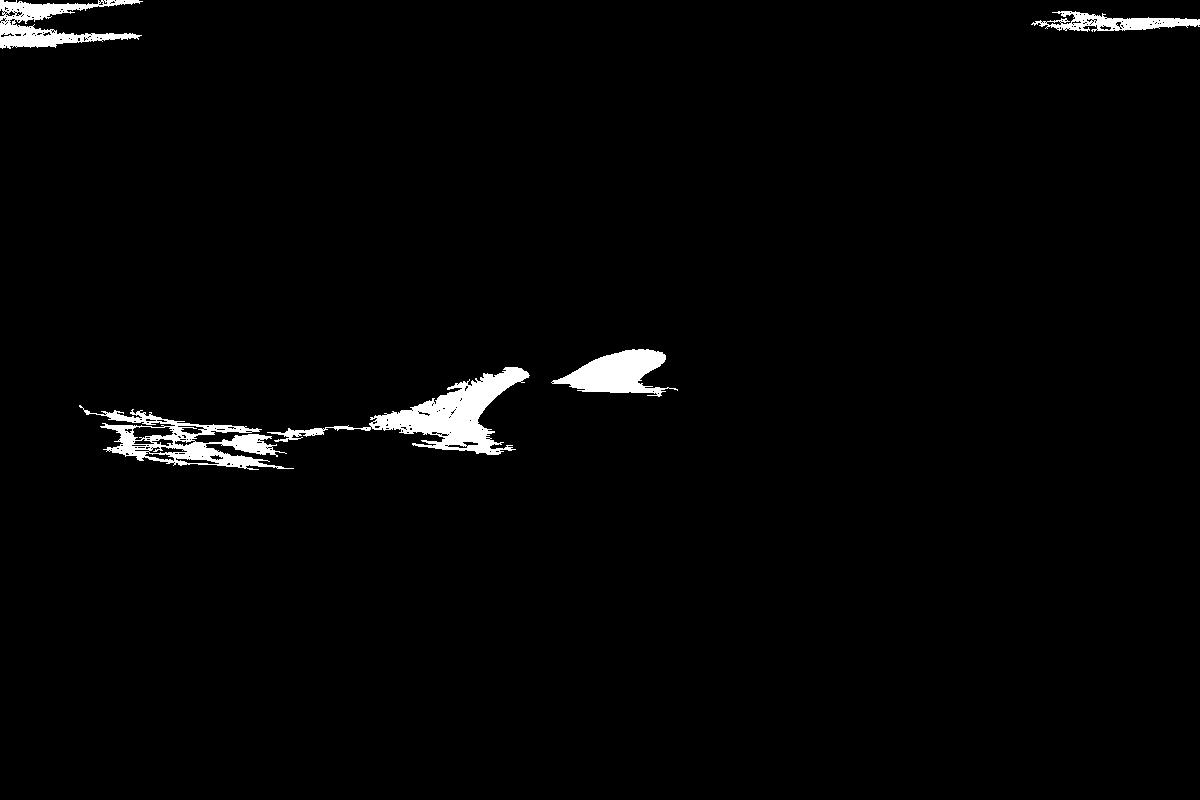
\includegraphics[width=\textwidth]{dopoFiltroFoto.jpg}
  \caption{Prima dell'individuazione delle regioni connesse}
  \end{subfigure}
  
  \vspace{5mm}
  
  \begin{subfigure}[b]{0.3\textwidth}
    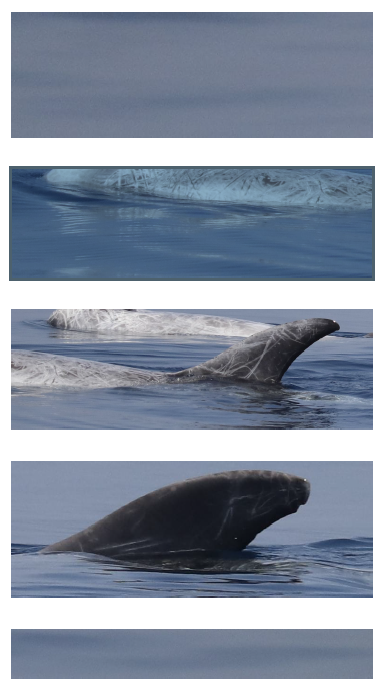
\includegraphics[width=0.95\textwidth]{ritaglioBlob.png}
  \caption{Estrazione
delle regioni connesse dall’immagine binarizzata}
  \end{subfigure}
  \begin{subfigure}[b]{0.3\textwidth}
    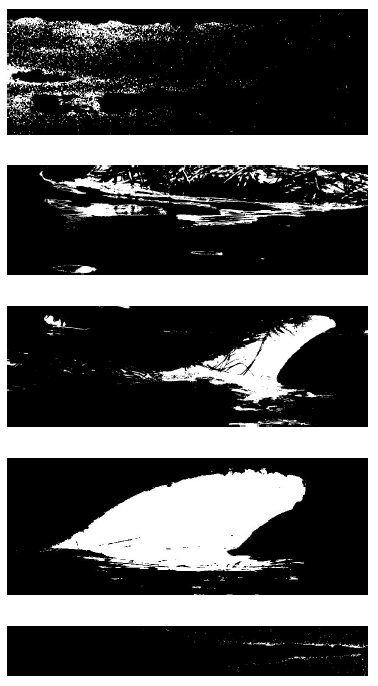
\includegraphics[width=0.95\textwidth]{dopoOtsuBlob.png}
  \caption{Applicazione ripetuta della sogliatura secondo Otsu (senza CLAHE)}
  \end{subfigure}
  \begin{subfigure}[b]{0.3\textwidth}
    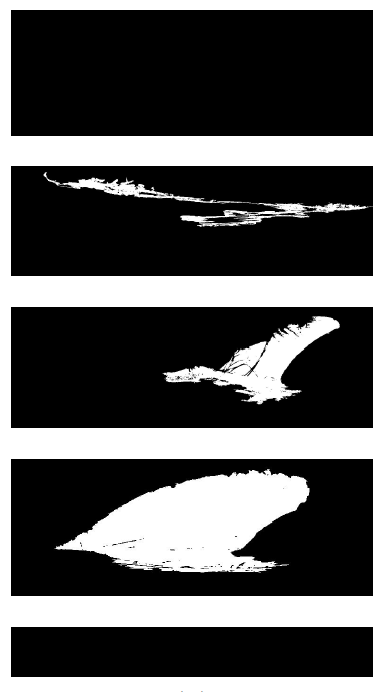
\includegraphics[width=0.95\textwidth]{dopoFiltroBlob.png}
  \caption{Applicazione del secondo filtro sulle regioni connesse estratte}
  \end{subfigure}
  
  \caption{Fase di filtraggio delle regioni connesse}
  \label{fig:filtraggioBlob}
\end{figure}

\subsection*{Ritaglio adattivo}
Le regioni binarie mantenute in seguito alla fase di filtraggio sono sottoposte ad un algoritmo che consente di ottenere un ritaglio preciso in corrispondenza delle pinne.
Tale operazione si può definire "adattiva" nella misura in cui la regione di ritaglio è ottenuta a partire da precisi punti geometrici calcolati per ciascuna regione binaria.
Evitando di scendere nei dettagli implementativi e numerici (riportati nel par. 5.1 in \cite{gianvito}), si descrivono nell'ordine le operazioni effettuate sulle singole regioni binarie dall'algoritmo di ritaglio:
\begin{enumerate}
\item Si sottopone la regione binaria al riempimento dei cosiddetti \textit{holes}, cioè "buchi" anneriti racchiusi in una regione connessa, mediante la funzione \verb|imfill| con opzione \verb|'holes'|
\item Si individuano quattro punti di interesse; nell’ordine: punto più in alto, punto medio tra questo ed il centroide, punti di estrema sinistra e destra della regione connessa all’altezza del
punto medio
\item Si identifica il più piccolo rettangolo che racchiude i punti precedentemente trovati
\item Si trasla e si estende il rettangolo trovato in modo che contenga l’intera pinna, a seconda della sua orientazione.
\end{enumerate}

L'output di questa prima fase della routine sono i ritagli di quelle regioni dell'immagine originale che, verosimilmente, ritraggono una pinna dorsale. Questa ipotesi sul contenuto dei ritagli è sostenuta solamente sulla base del processo di segmentazione e filtraggio appena descritto.\\

\noindent Il risultato dell'operazione è visualizzato in figura \ref{fig:ritaglioAdattivo}\\

\begin{figure}[h!]

  \centering
  
  \begin{subfigure}[t]{0.475\textwidth}
    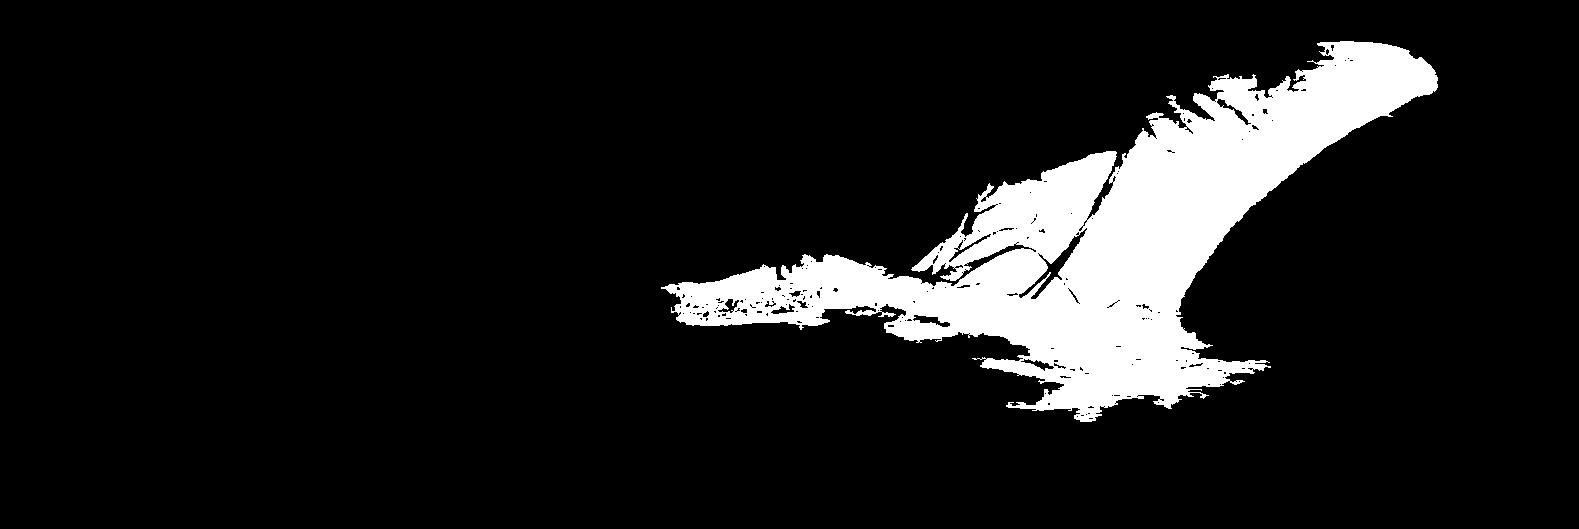
\includegraphics[width=0.95\textwidth]{ritaglio1.jpg}
    \caption{Regione binaria da sottoporre a ritaglio adattivo}
  \end{subfigure}
  \begin{subfigure}[t]{0.475\textwidth}
    
\includegraphics[width=0.95\textwidth]{ritaglio2.jpg}
    \caption{Riempimento degli \textit{holes}}
  \end{subfigure}
  
  \vspace{5mm}
  
  \begin{subfigure}[b]{0.7\textwidth}
    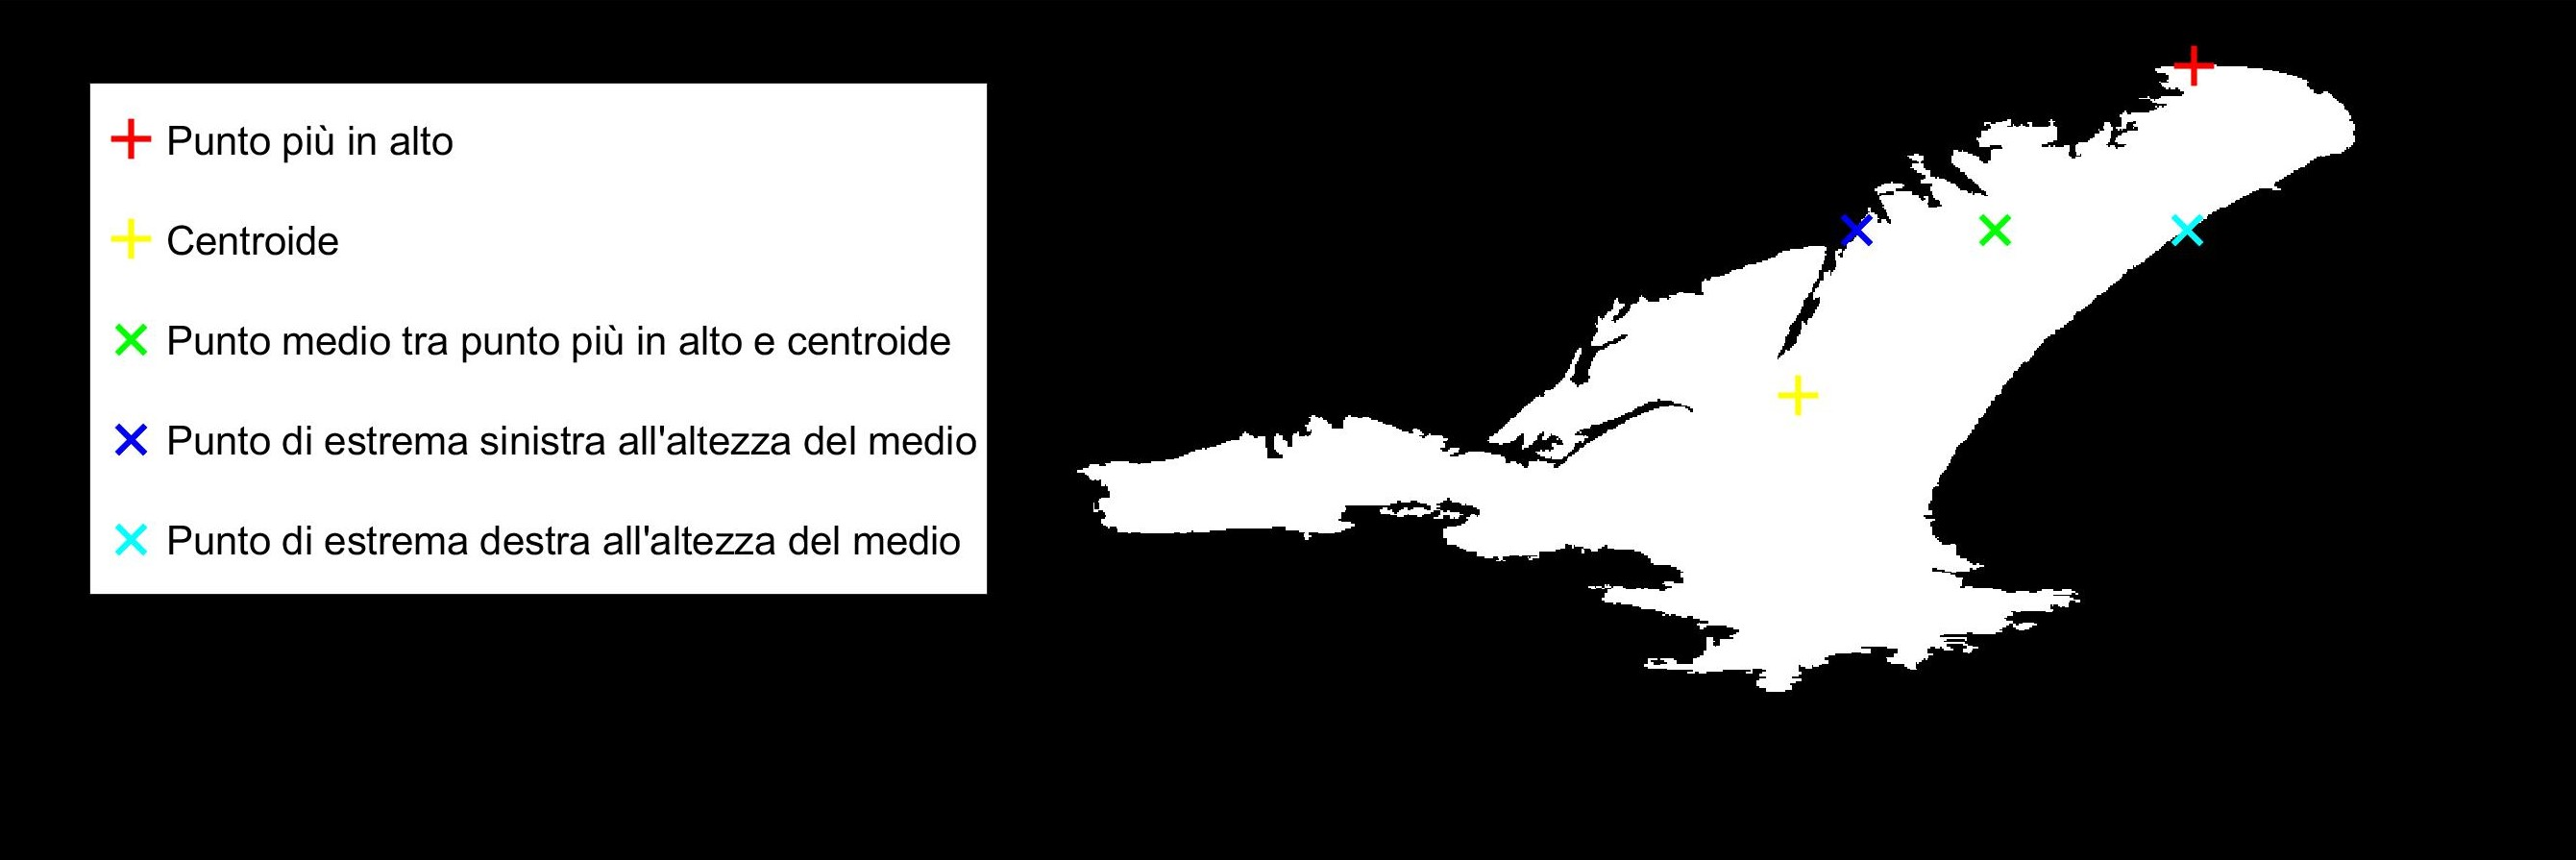
\includegraphics[width=\textwidth]{ritaglio3.jpg}
    \caption{Individuazione dei quattro punti di interesse}
  \end{subfigure}
  
  \vspace{5mm}
  
  \begin{subfigure}[b]{0.7\textwidth}
    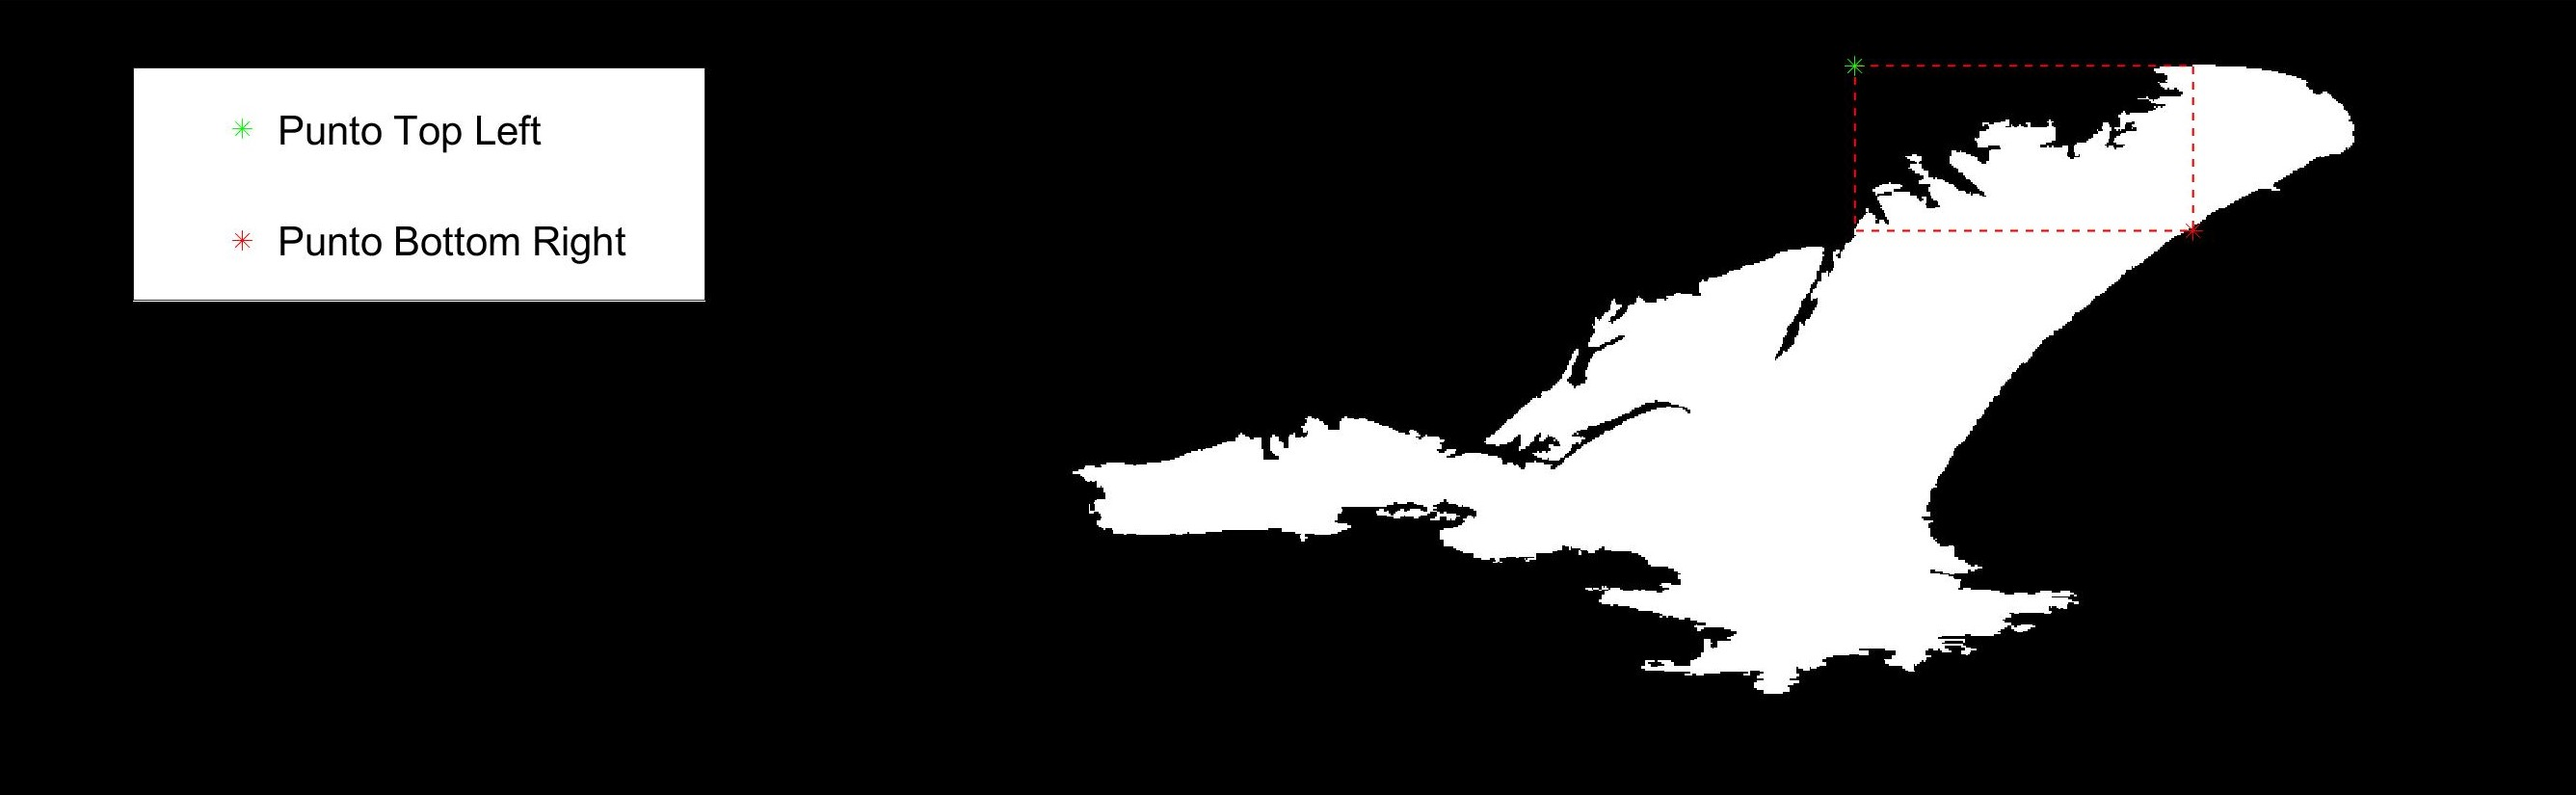
\includegraphics[width=\textwidth]{ritaglio4.jpg}
    \caption{Individuazione del rettangolo che racchiude i quattro punti di interesse}
  \end{subfigure}
  
  \vspace{5mm}
  
  \begin{subfigure}[b]{0.7\textwidth}
    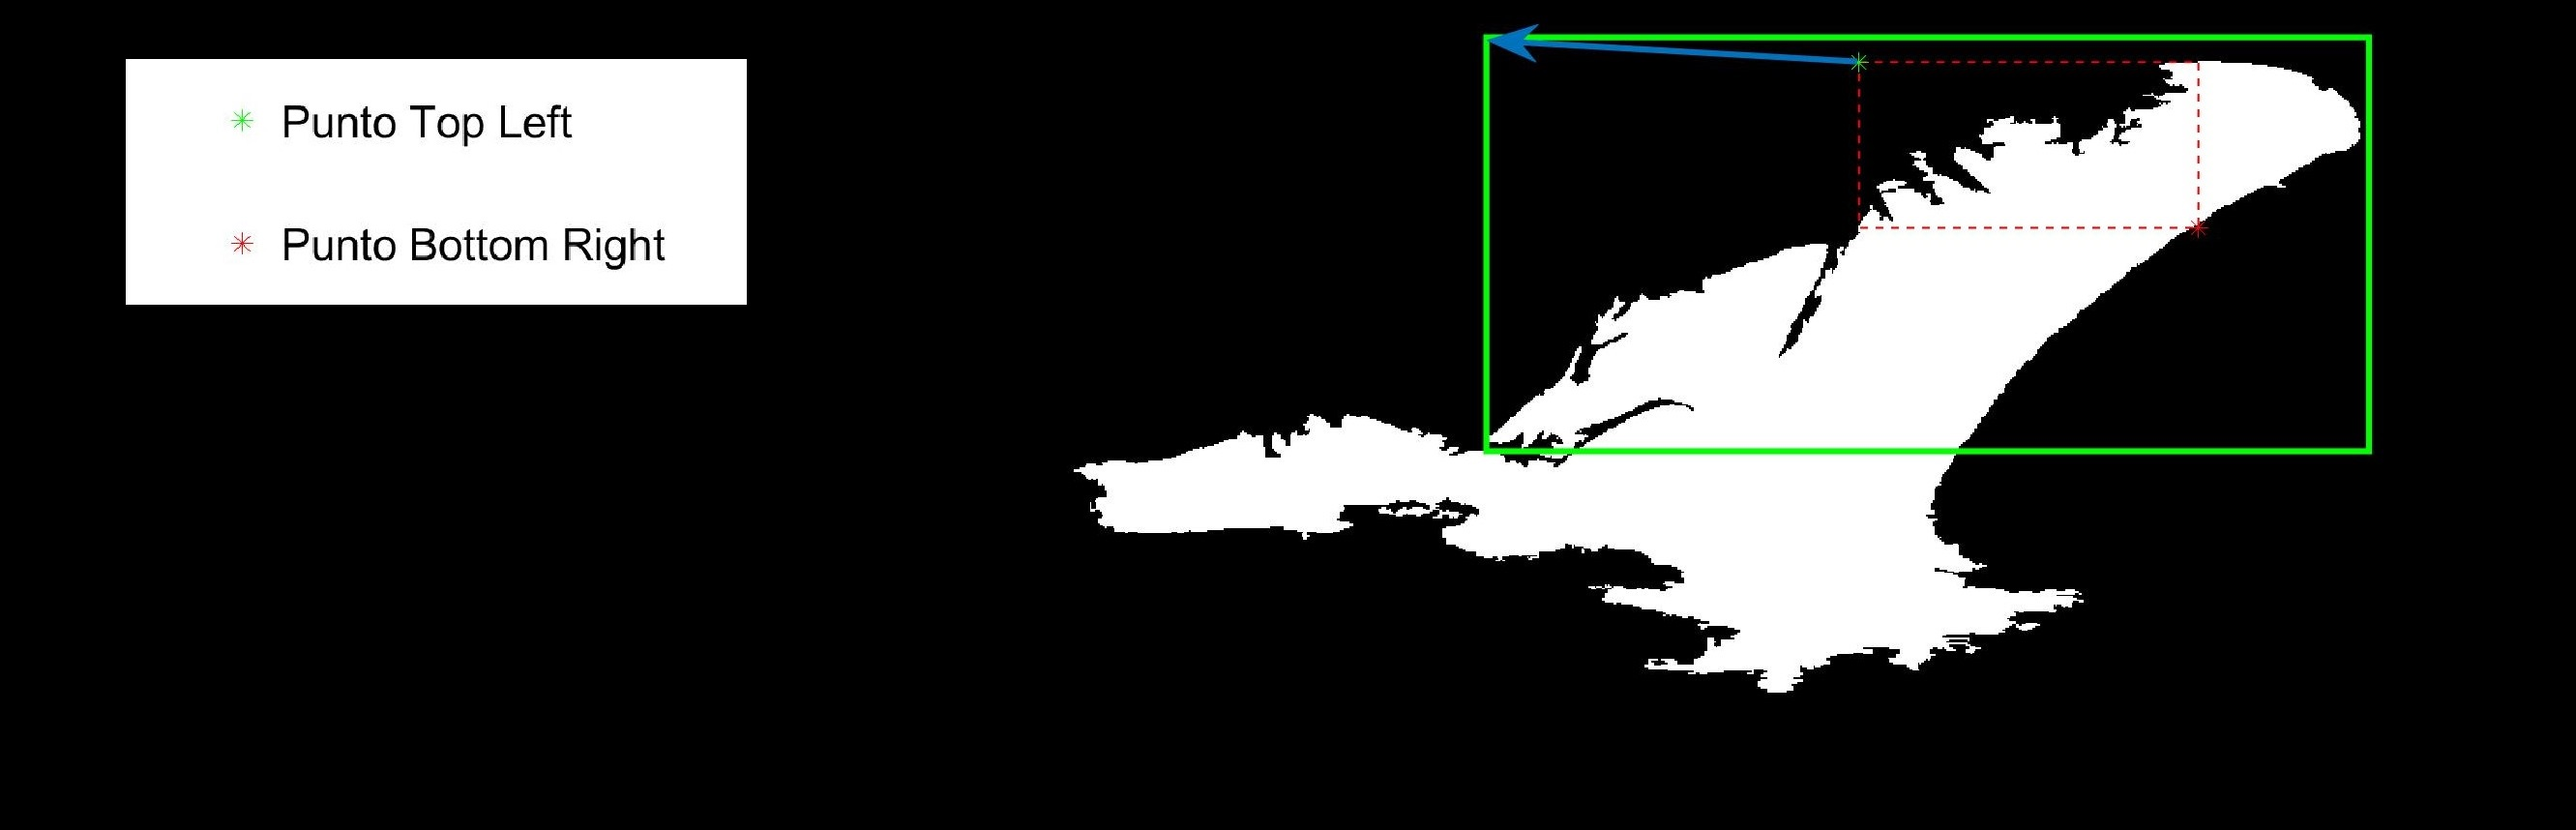
\includegraphics[width=\textwidth]{ritaglio5.jpg}
    \caption{Traslazione ed estensione del rettangolo trovato}
  \end{subfigure}
  
  \vspace{5mm}
  
  \begin{subfigure}[b]{0.475\textwidth}
    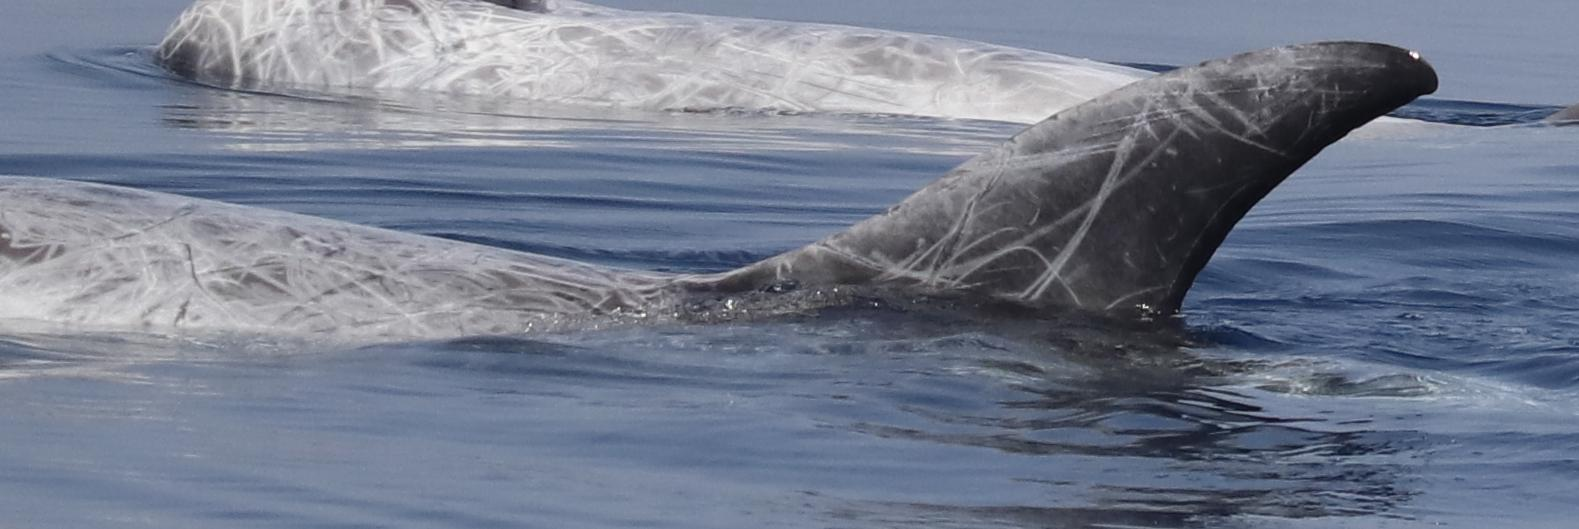
\includegraphics[width=0.95\textwidth]{ritaglio6.jpg}
    \caption{Ritaglio di partenza}
  \end{subfigure}
  \begin{subfigure}[b]{0.475\textwidth}
    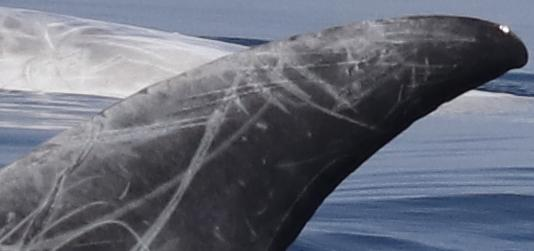
\includegraphics[width=0.95\textwidth]{ritaglio7.jpg}
    \caption{Risultato finale}
  \end{subfigure}
  
  \caption{Fase di ritaglio adattivo}
  \label{fig:ritaglioAdattivo}
\end{figure}

La routine CropFin v1, nella sua prima fase di ritaglio adattivo, è stata applicata ai dataset degli scatti di Taranto e delle Azzorre. In tabella \ref{risultatiCrop} è riportato il numero di ritagli (\textit{crops}) prodotti da CropFin v1 con input i dataset sopracitati.

\begin{table}[h]

  \centering
  \begin{tabular}{c c c c c}
  \hline
  Dataset&N. foto&N. crop&di cui 'Pinna'&di cui 'No Pinna'\\
  \hline
  Taranto&10194&15228&4033&11195\\
  Azzorre&11290&20395&3793&16602\\
  \hline
  \end{tabular}
  
  \caption{Output della prima fase di CropFin v1}
  \label{risultatiCrop}

\end{table}

\subsection{Fase di classificazione}
\label{faseClassificazione}

È evidente da una rapida ispezione dell'output che la quantità di regioni estratte che però non contengono pinne risulta, su larga scala, superiore a quella che contiene effettivamente pinne. Numericamente questo fatto è evidenziato in tab. \ref{risultatiCrop}, compilata dopo una fase di etichettatura a mano dei ritagli prodotti, nelle classi 'Pinna' e 'No Pinna' (motivata e spiegata nel seguito del sottoparagrafo). I ritagli della classe 'No Pinna' ottenuti sono l’esito "fallimentare" della procedura di segmentazione, filtraggio e ritaglio adattivo adottati in CropFin v1.

Questa osservazione è ciò che primariamente motiva l’introduzione di una fase di classificazione finale in CropFin v1, che consenta di automatizzare completamente la procedura di object detection.\\

La fase di classificazione prevede l'impiego di un classificatore binario che sappia discriminare un ritaglio in 'Pinna' o 'No Pinna'. L'addestramento di un tale classificatore (a prescindere dalle sue caratteristiche) può essere fatto mediante tecniche di supervised learning (par. \ref{supervisedLearning}), avendo a disposizione molti esempi "etichettati" di entrambe le classi da predire.

\subsection*{Creazione del training set}

Per consentire l'addestramento del classificatore si rende quindi necessario un lavoro di etichettatura manuale dei ritagli, attribuendo a ciascuno la classe 'Pinna' e 'No Pinna'. Questa operazione è stata svolta per entrambi i dataset a nostra disposizione; i risultati di questa etichettatura manuale sono presenti nella tab. \ref{risultatiCrop}.\\

Si precisa che, nella fase di etichettatura manuale, sono stati attribuiti alla classe 'Pinna' tutti e soli i ritagli contenenti una sola pinna in primo piano, intera o leggermente tagliata, escludendo invece quelli con pinne multiple e quelli con una presenza preponderante del dorso dei delfini. I ritagli con tali caratteristiche, infatti, sono considerati maggiormente affidabili ai fini di una successiva foto-identificazione automatica delle pinne (ad esempio con la routine "\textit{SPIR}" sviluppata e descritta in \cite{maglietta} e migliorata in \cite{emanuele}). Inoltre, questa scelta è stata anche motivata dall’intenzione di creare un "concetto univoco" utile a semplificare sia la selezione manuale sia l’apprendimento del classificatore.
In fig. \ref{fig:esempiPinnaNoPinna} sono riportati alcuni esempi di etichettatura dei ritagli.

\begin{figure}[h!]

  \centering
  
  \begin{subfigure}[b]{0.7\textwidth}
    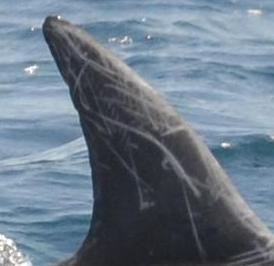
\includegraphics[width=0.19\textwidth]{p1.jpg}
    \hfill
    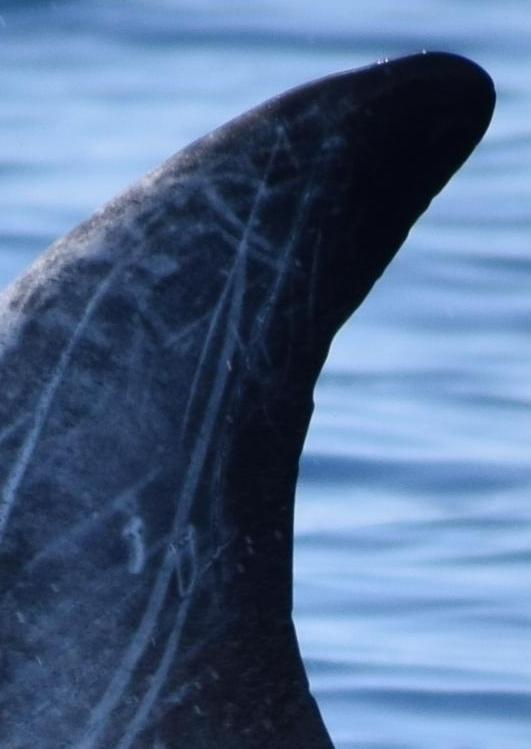
\includegraphics[width=0.19\linewidth]{p2.jpg}
    \hfill
    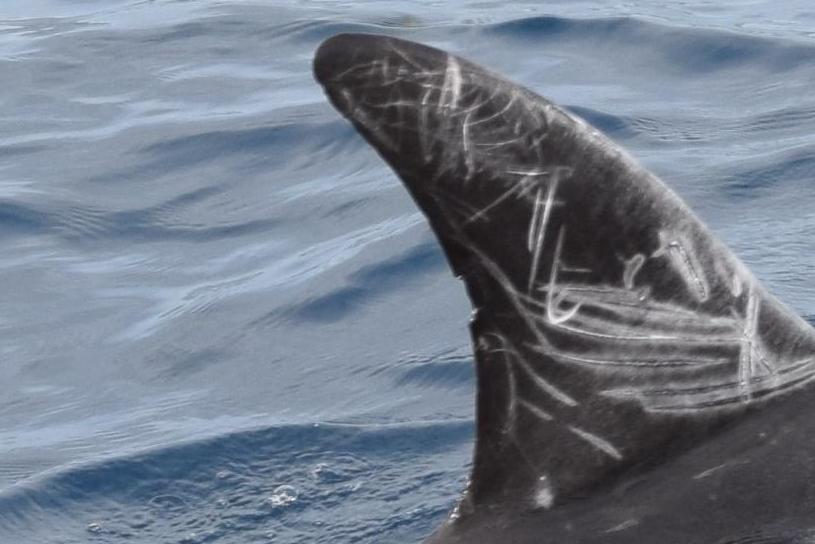
\includegraphics[width=0.19\linewidth]{p3.jpg}
    \hfill
    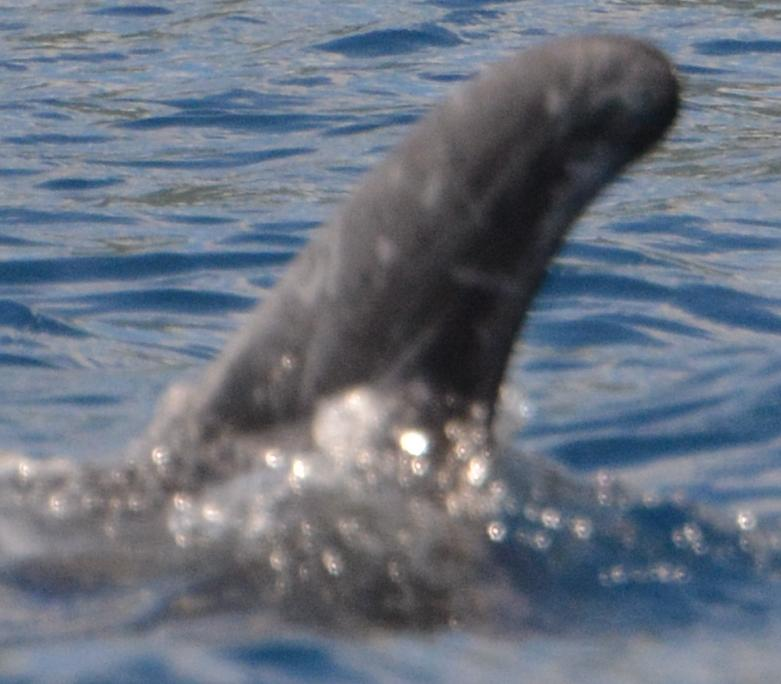
\includegraphics[width=0.19\linewidth]{p4.jpg}
    \hfill
    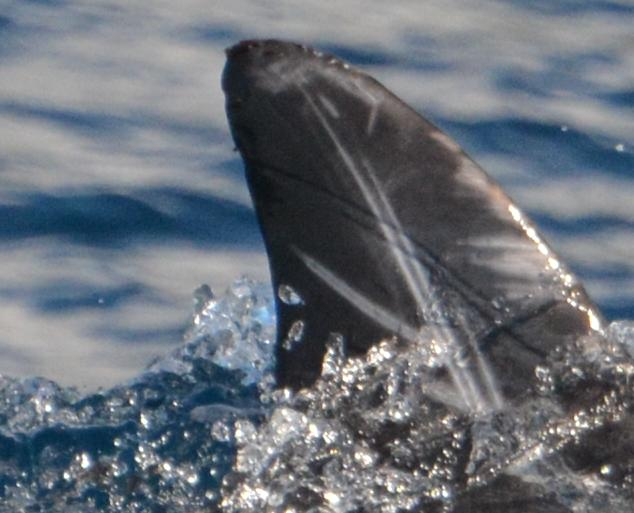
\includegraphics[width=0.19\linewidth]{p5.jpg}
    \caption{}
  \end{subfigure}
  
  \vspace{5mm}
  
  \begin{subfigure}[b]{0.7\textwidth}
    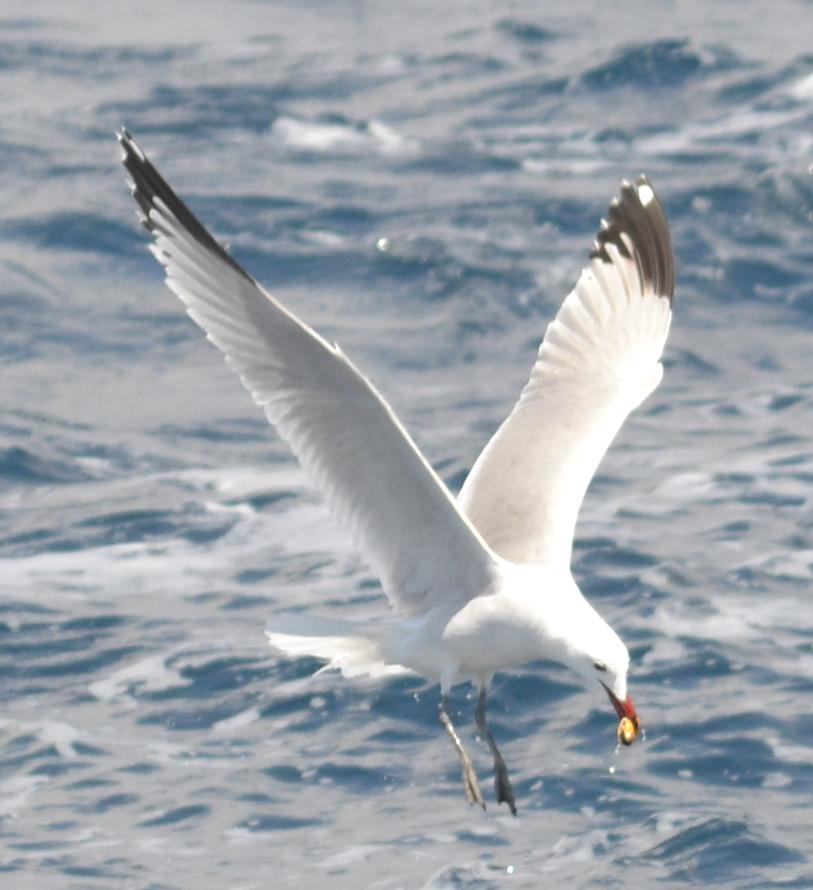
\includegraphics[width=0.19\textwidth]{np1.jpg}
    \hfill
    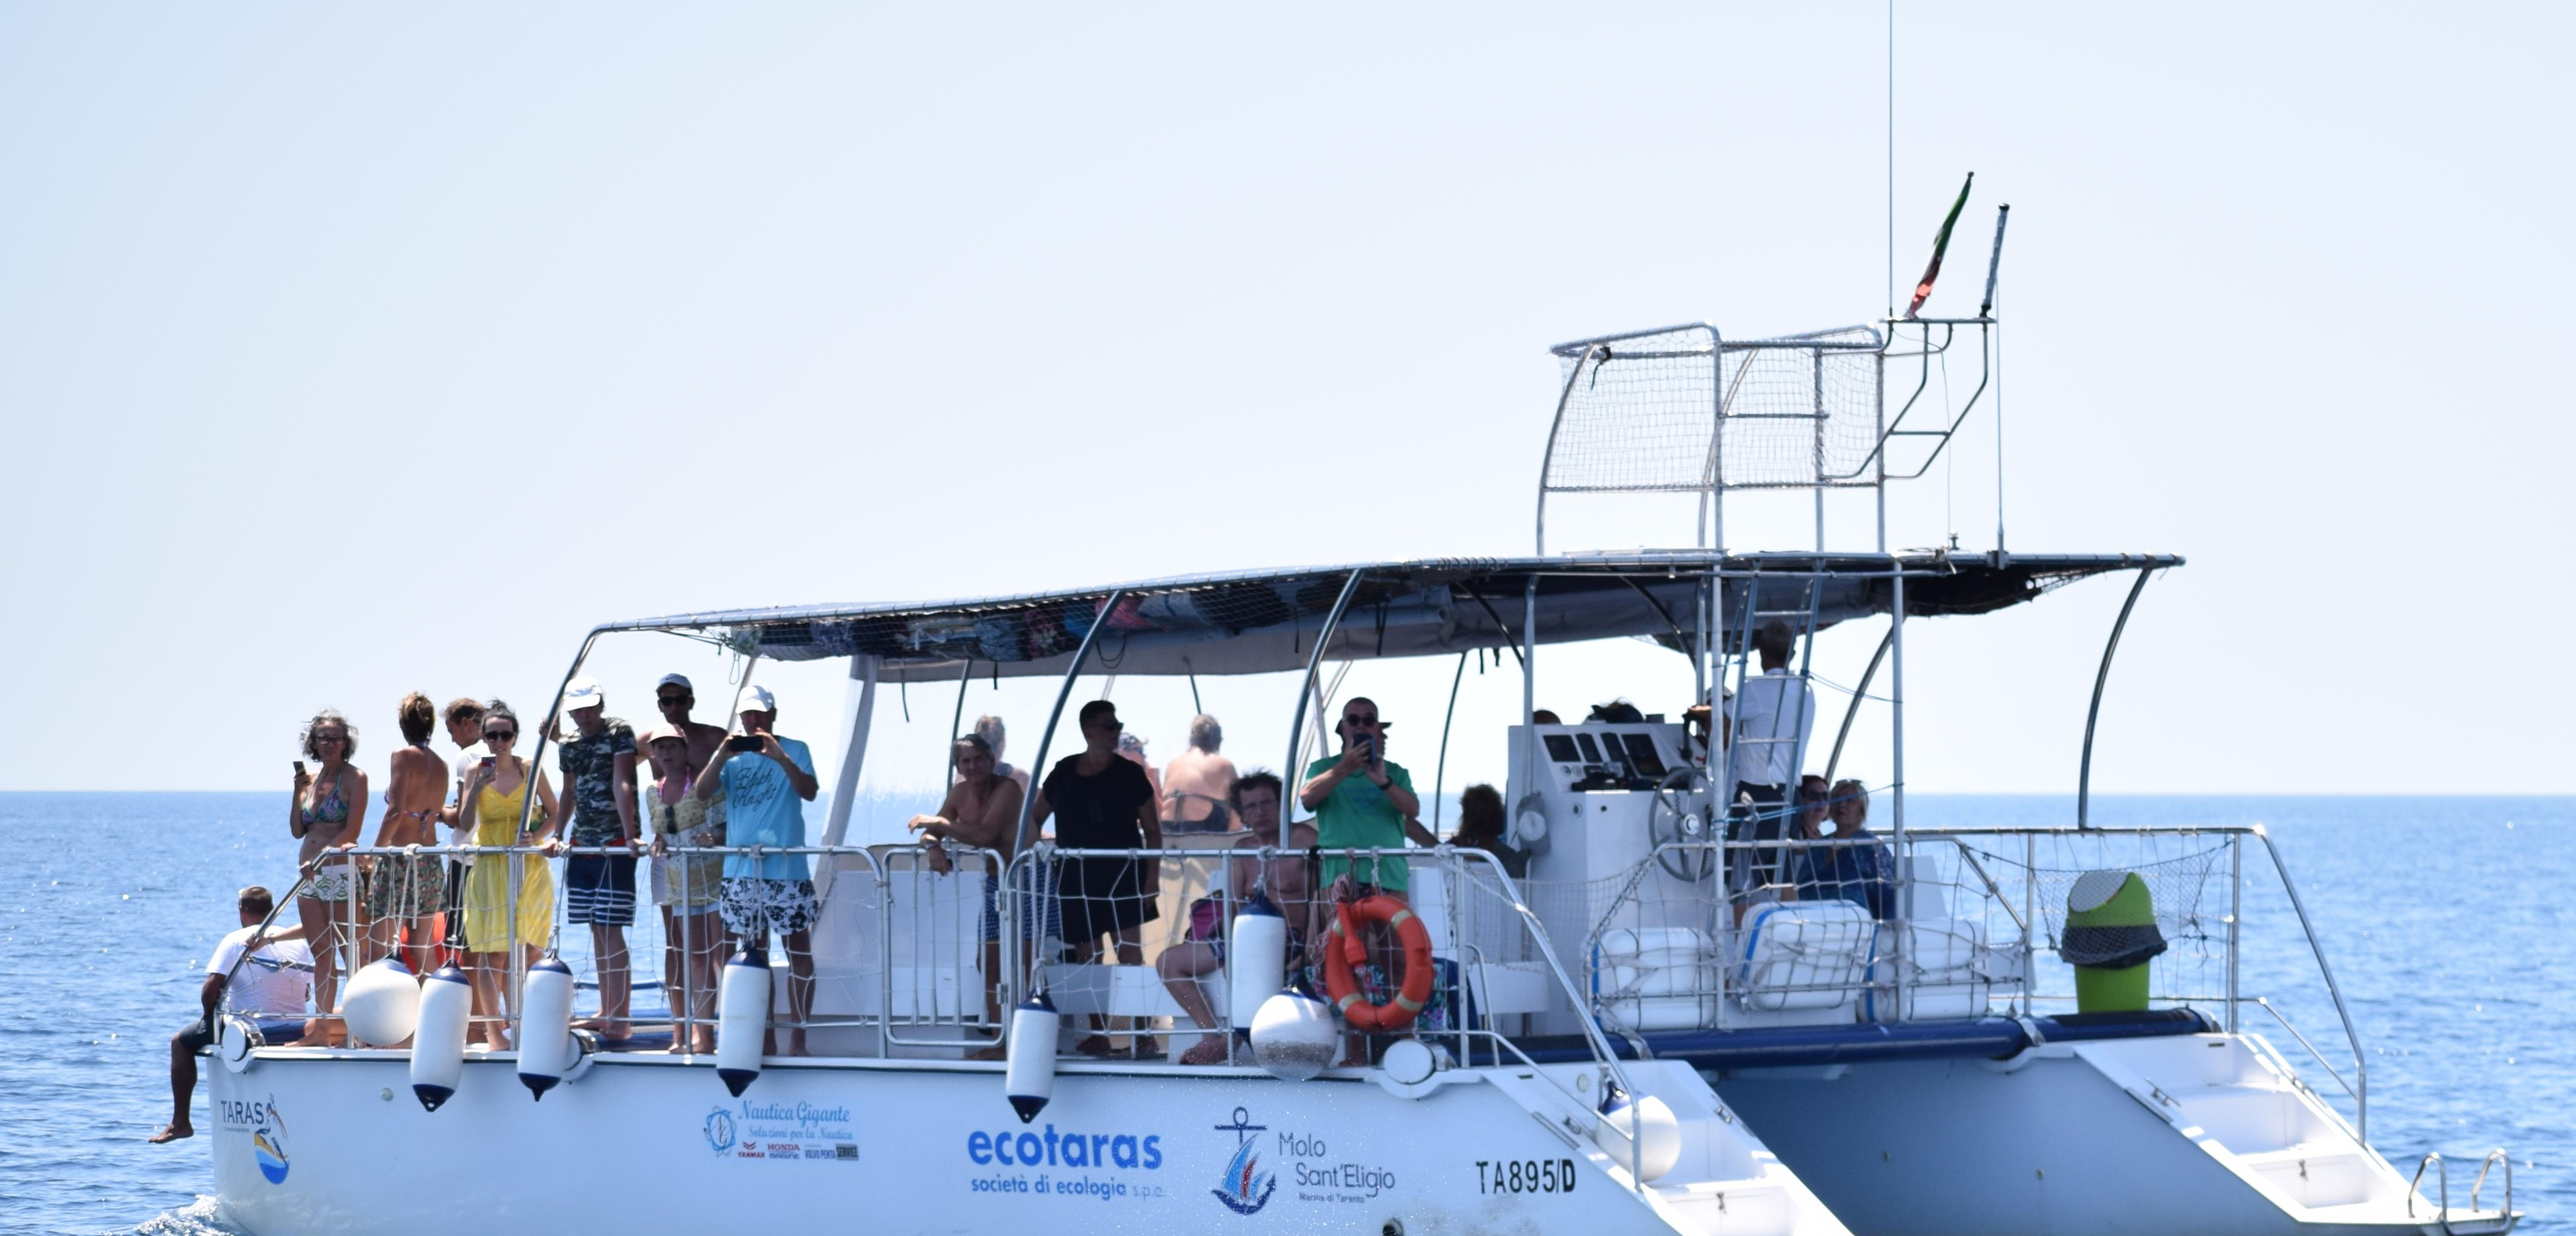
\includegraphics[width=0.19\linewidth]{np2.jpg}
    \hfill
    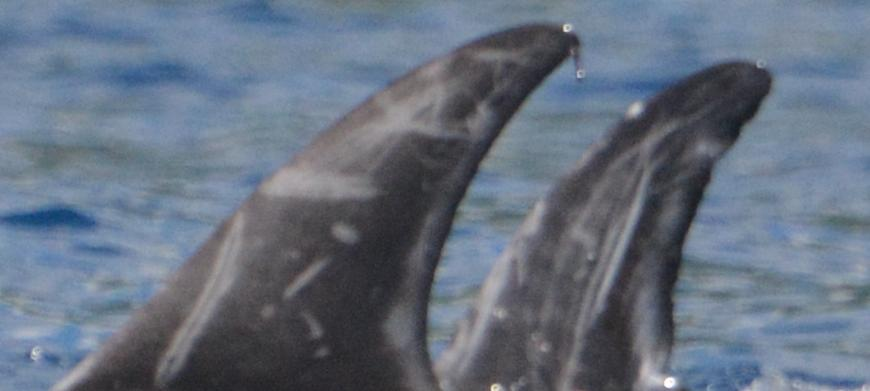
\includegraphics[width=0.19\linewidth]{np3.jpg}
    \hfill
    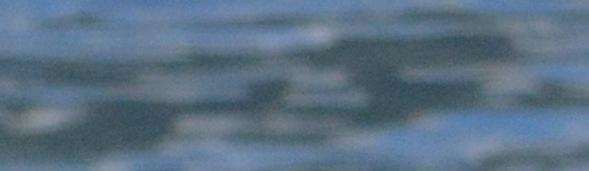
\includegraphics[width=0.19\linewidth]{np4.jpg}
    \hfill
    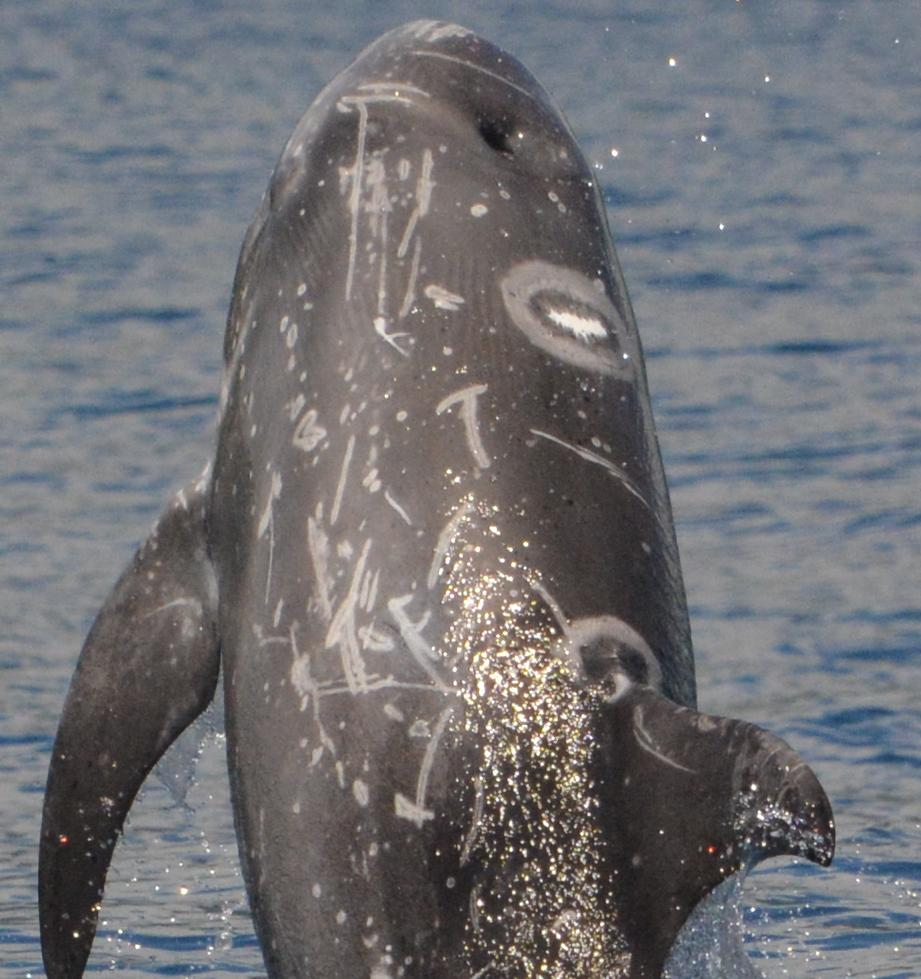
\includegraphics[width=0.19\linewidth]{np5.jpg}
    \caption{}
  \end{subfigure}
  
  \caption{Alcuni ritagli etichettati manualmente come appartenenti alla classe (a) 'Pinna', (b) 'No Pinna'}
  \label{fig:esempiPinnaNoPinna}
\end{figure}

I due dataset così etichettati si prestano bene ad essere usati per addestrare un classificatore in grado di risolvere il task in esame.

\subsection*{Classificazione mediante rete \textit{ad-hoc}}
Tra i vari modelli di classificazione adottabili, in CropFin v1 si decide di progettare una rete neurale convoluzionale creata \textit{ad-hoc}, costruita cioè appositamente per risolvere il task in questione, da zero (\textit{from scratch}). L'addestramento del classificatore è avvenuto con i 15228 ritagli del dataset di Taranto.
Per i dettagli sull'architettura, l'addestramento e le prestazioni di questo classificatore \textit{ad-hoc} si rimanda al par. 4.4.2 di \cite{gianvito}.\\

In questo lavoro di tesi si è tentato un approccio diverso alla classificazione: si è provato a risolvere il task mediante il riutilizzo di CNN pre-addestrate, con la tecnica del \textit{Transfer Learning}.


\section{Classificazione mediante CNN e Transfer Learning}
\label{esperimentoTL}
Nel par. \ref{transferLearning} sono state esposte molteplici motivazioni per le quali per risolvere un problema di classificazione (in particolare di \textit{image classification}) può essere meglio usare la tecnica del \textit{transfer learning}, adattando al task in esame una rete neurale pre-addestrata piuttosto che creare una rete da zero.
Il nucleo principale di questo lavoro di tesi è quindi dedicato alla creazione di un nuovo modello di classificazione, basato su \textit{transfer learning}, che possa migliorare la fase di classificazione di CropFin v1. Questi "miglioramenti" sono da valutare con rigore ingegneristico sulla base di alcuni parametri, che consentono un confronto di prestazioni con il classificatore di CropFin v1; l'analisi delle prestazioni e quindi il confronto è svolto nel par. \ref{classEnsemble}.

\subsection{Scelta delle CNN}
Sono state riutilizzate ed adattate mediante la tecnica del \textit{transfer learning} quattro reti neurali convoluzionali (\textit{CNN}) sviluppate nell'ambito della \textit{ImageNet Large Scale Visual Recognition Challenge (ILSVRC)} ed addestrate sul dataset ImageNet (par. \ref{imagenet}). La loro scelta è stata motivata dal loro successo e prestigio nell'ambito del problema di \textit{object classification} proposto nella \textit{ILSVRC}. La scelta di queste reti è stata altresì motivata da un interesse puramente didattico, cioè studiare il funzionamento di CNN diverse per scelte architetturali e prestazioni, a prescindere dalla risoluzione del problema in esame. Esse sono di seguito elencate

\begin{itemize}

\item \textbf{AlexNet} (par. \ref{alexnet})\\
La sua vittoria nella \textit{ILSVRC 2012} con un tasso di errore \textit{top-5} del 16.4\% ha di fatto dimostrato alla comunità scientifica la straordinaria efficienza delle reti neurali convoluzionali nell'ambito dei problemi di \textit{computer vision}.

\item \textbf{GoogLeNet} (par. \ref{googlenet})\\
Grazie all'introduzione del modulo \textit{Inception}, GoogLeNet è una rete profonda ma incredibilmente leggera e semplice da addestrare, se paragonata alle precedenti reti fino ad allora esistenti (tra tutte, AlexNet).

\item \textbf{ResNet-18} (par. \ref{resnet})\\
ResNet rappresenta lo stato dell'arte nell'ambito delle reti neurali convoluzionali; l'introduzione dei \textit{residual blocks} ha permesso di avere reti con un grandissimo numero di layer, attenuando di molto i problemi legati all'estrema profondità dell'architettura.

\item \textbf{ResNet-50} (par. \ref{resnet})\\
Una variante di ResNet, più profonda e con migliori prestazioni sul dataset \textit{ImageNet}.

\end{itemize}

\subsection{Addestramento}
\label{addestramento}
L'ambiente di sviluppo nel quale sono state addestrate le quattro reti è il software Matlab R2019a, esteso con il pacchetto \textit{Deep Learning Toolbox}. Tutto il codice sorgente Matlab creato è riportato nel cap. \ref{sorgenti}.\\

Il dataset utilizzato per l'addestramento è quello con gli $n=15228$ ritagli che CropFin ha prodotto dagli scatti di Taranto (vd. tab. \ref{risultatiCrop}) e in seguito opportunamente etichettati a mano (come descritto nel par. \ref{faseClassificazione}). Questo dataset è di fatto lo stesso usato per l'addestramento del classificatore \textit{ad-hoc} in \cite{gianvito}.

Il dataset dei ritagli è rappresentato in Matlab da un oggetto \verb|imageDatastore|, ed è stato suddiviso (\textit{splitted}) in maniera casuale in due ulteriori oggetti \textit{imageDatastore}:

\begin{itemize}
\item \begin{frame}\space \verb|cropTrain|\end{frame}, un \textit{training set} contenente il 70\% dei ritagli (10659 ritagli), cioè il 70\% dei ritagli 'No Pinna' (7836) più il 70\% dei ritagli 'Pinna' (2823)
\item \begin{frame}\space \verb|cropValidation|\end{frame}, un \textit{validation set} contenente il rimanente 30\% dei ritagli (4569 ritagli di cui 3359 'No Pinna' e 1210 'Pinna')
\end{itemize}

Il training set è sottoposto ad operazioni di \textit{image augmentation} durante la fase di addestramento, per migliorare la capacità di generalizzazione del classificatore da addestrare ed evitare quindi l'\textit{overfitting}.
A ciascuna immagine del set sono applicate le seguenti trasformazioni, rappresentate in un opportuno oggetto \verb|imageDataAugmenter|:

\begin{itemize}
\item una riflessione rispetto all’asse x (operata con il 50\% di probabilità);
\item una rotazione di un angolo casualmente estratto dall’intervallo $[-20, 20]$ gradi;
\item una traslazione sull’asse x di una quantità casualmente estratta dall’intervallo
$[-60, 60]$ pixel.
\end{itemize}

\noindent Un oggetto \verb|augmentedImageDatastore| parametrizzato con l'\verb|imageDataAugmenter| sopra descritto e l'\verb|inputSize| della rete è creato per rappresentare la versione "aumentata" di \verb|cropTrain|.
Le operazioni applicate in maniera casuale contribuiscono ad ottenere ulteriore variabilità del dataset impiegato per la fase di addestramento; i ritagli vengono inoltre ridimensionati all'input size della rete da addestrare. Si è ritenuto opportuno impiegare poche trasformazioni ad effetto limitato: le uniche che non alterassero eccessivamente il contenuto dei ritagli di classe Pinna rispetto al problema in esame ed al dataset a disposizione (già di per sè contenente grande variabilità relativa alla classe Pinna).

\begin{figure}[h!]
  \centering
  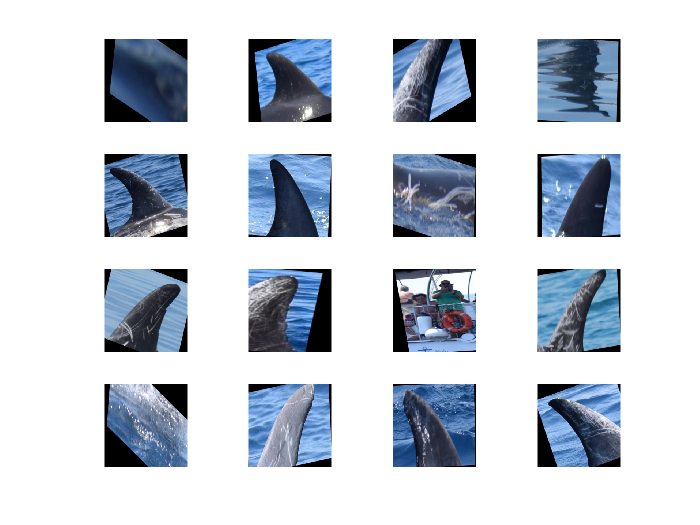
\includegraphics[width=0.75\textwidth]{augmentation.png}
  \caption{Un campione di ritagli sottoposti alle operazioni di \textit{augmentation}}
  \label{fig:augmentation}
\end{figure}

Un secondo oggetto \verb|augmentedImageDatastore| è usato per rappresentare \verb|cropValidation|, ma in questo caso parametrizzato solo con \verb|inputSize|, viene cioè effettuato solamente un ridimensionamento dei ritagli all'input size della rete da addestrare, senza operazioni di augmentation.

Si noti che i due dataset "aumentati" hanno le stesse dimensioni dei loro omologhi dataset "non aumentati", nel senso che ogni ritaglio del dataset originale è presente esattamente una volta nel relativo dataset aumentato: l'unica differenza tra il ritaglio originale e quello nel dataset aumentato è appunto l'applicazione (a \textit{runtime}) delle operazioni di ridimensionamento e (nel caso del \textit{training set}) augmentation a ciascun ritaglio. Si tratta quindi di una semplice "perturbazione" dei due dataset, senza eliminazione di suoi elementi o aggiunta di nuovi.\\

L'inizializzazione delle quattro CNN all'interno dell'ambiente Matlab è particolarmente semplice, e può essere effettuato richiamando la rete col suo nome (\verb|alexnet|, \verb|googlenet|, \verb|resnet18|, \verb|resnet50|) assegnandola ad una variabile, avendo cura di scaricare il relativo \textit{add-on} dall'\textit{add-on explorer} integrato di Matlab, estendendo il \textit{Deep Learning Toolbox}.

Le quattro reti, come visto nei rispettivi paragrafi, sono in origine state addestrate sul database di immagini \textit{ImageNet} (par. \ref{imagenet}) per classificare un'immagine scegliendo tra le mille categorie diverse del dataset. Applicare la tecnica del \textit{transfer learning} (par. \ref{transferLearning}) per adattare ciascuna rete al problema di classificazione binaria delle pinne significa effettuare le seguenti operazioni

\begin{itemize}
\item analizzare l'architettura della rete e decidere quanti e quali layer (tra quelli dotati di parametri addestrabili) "congelare", cioè impedirne l'ulteriore \textit{fine-tuning} dei  parametri in fase di ri-addestramento azzerando il learning rate dei layer
\item sostituire nella rete originale da "trasferire" l'ultimo \textit{fully-connected layer} avente 1000 neuroni, ognuno associato alle 1000 classi del database ImageNet e il cui valore di attivazione permette di calcolare la probabilità per la relativa classe (attraverso la funzione \textit{softmax}), con un nuovo \textit{fully-connected layer} dotato di 2 soli neuroni, relativi alle classi 'Pinna' e 'No Pinna'; questo nuovo layer è inizializzato con un learning rate abbastanza alto (fissato a 10) per permettere un addestramento più veloce
\item adattare la nuova rete così creata al problema di classificazione binaria delle pinne grazie al ri-addestramento della rete sul nuovo dataset dei ritagli, descritto in precedenza
\end{itemize}

Si noti che per la scelta di quanti e quali layer parametrizzati "congelare" non esistono regole o criteri generali; questa scelta è un nuovo set di iperparametri della rete, da trovare risolvendo uno specifico problema di ottimizzazione degli iperparametri. Poiché per ottimizzare questi iperparametri sarebbe necessario addestrare un gran numero di volte ciascuna delle quattro reti, con un notevole impiego di tempo, tale problema di ottimizzazione non è stato risolto in questa sede e si è preferito scegliere manualmente i layer da congelare.

Per garantire un buon \textit{trade-off} tra capacità di generalizzazione sul nuovo dataset e velocità di addestramento della rete, si è scelto di congelare uno, due o tre layer convoluzionali iniziali di ciascuna rete, nell'ordine in cui sono presenti nell'architettura della rete.
Tale scelta è motivata anche dal fatto che il dataset \textit{ImageNet} e quello dei ritagli delle pinne hanno alcune caratteristiche in comune: nel primo ci sono almeno una decina di classi diverse di cetacei, come ad esempio 'gray whale' (balena grigia) e 'killer whale' (orca).
Mutuando un'idea discussa in \cite{howtransferable}, si è quindi avanzata la plausibile ipotesi che tutte le reti abbiano imparato, nei livelli più bassi, ad estrarre \textit{features} abbastanza generali utili per il riconoscimento di una variegata classe di animali marini e delle loro parti del corpo, e pertanto questi primi layer possono essere riutilizzati senza modifiche.
Per ulteriori dettagli sull'implementazione in Matlab riferirsi al cap. \ref{sorgenti}.\\

Per ogni classificatore, l’addestramento è stato eseguito con il metodo \textit{stochastic gradient descent with momentum}, con dimensione del \textit{minibatch} pari a 20, numero di epoche pari a 6 e \textit{learning rate} globale pari a 0.0003.
Ciò ha portato alla definizione del seguente oggetto \verb|trainingOptions|:

\begin{verbatim}
miniBatchSize = 20;
valFrequency = floor(numel(cropAugmentedTrain.Files)/miniBatchSize);

options = trainingOptions('sgdm', ...
    'MiniBatchSize',miniBatchSize, ...
    'MaxEpochs',6, ...
    'InitialLearnRate',3e-4, ...
    'Shuffle','every-epoch', ...
    'ValidationData', cropAugmentedValidation, ...
    'ValidationFrequency',valFrequency, ...
    'Verbose',true, ...
    'Plots','training-progress', ...
    'CheckpointPath','.\Checkpoint [nome della rete]');
\end{verbatim}

Il numero di epoche di addestramento, relativamente basso, è accettabile in quanto utilizzando il transfer learning per ri-addestrare una rete pre-addestrata tipicamente sono necessarie poche iterazioni sull'intero dataset per ottenere un buon adattamento della rete al nuovo task di classificazione\footnote{come evidenziato in \url{https://it.mathworks.com/help/deeplearning/examples/transfer-learning-using-alexnet.html}}; inoltre un numero basso di epoche, assieme alle operazioni di augmentation, garantisce una discreta robustezza contro l'\textit{overfitting}, problema in cui si può facilmente incappare in presenza di un dataset di dimensioni relativamente ridotte come in questo caso.

Per quanto riguarda gli altri iperparametri (\textit{learning rate} globale e dimensione del \textit{minibatch}), i loro valori sono stati scelti empiricamente, sulla base di alcune \textit{best practices} generali presenti in letteratura\textsuperscript{3}, che funzionano bene con un'ampia classe di reti neurali convoluzionali e di dataset.
A rigore, i valori migliori per questi iperparametri possono essere trovati con la risoluzione di un preciso problema di ottimizzazione (che richiederebbe numerosi ri-addestramenti per ogni rete, con notevole dispendio di tempo). Tuttavia, come sarà evidente al momento della presentazione dei risultati, le prestazioni registrate dalle reti con questi iperparametri sono eccellenti, e non è necessario cercarne di migliori (un tale sforzo computazionale e di tempo non giustificherebbe un leggerissimo aumento dell'accuratezza).\\

\noindent L’addestramento di ciascuna rete è stato lanciato mediante la funzione
\begin{verbatim}
TL_net = trainNetwork(cropAugmentedTrain,layers,options)
\end{verbatim}
specificando il \textit{training set} sottoposto ad \textit{augmentation}, l’architettura della rete (array di tipo \verb|Layer| nel caso di AlexNet e di tipo \verb|LayerGraph| per le restanti reti) e le opzioni per l'addestramento.\\

\noindent Nella tabella \ref{prestazioniReti} sono riassunte le principali informazioni e i risultati globali (accuratezza sul \textit{validation set} e dati della matrice di confusione) di ciascuna rete così addestrata. Nelle figure dalla \ref{graficoAlexnet} alla \ref{graficoResnet50} sono riportati i grafici che mostrano l'andamento temporale dei quattro addestramenti.
L'addestramento è avvenuto nella modalità a singolo processore grafico su due diverse macchine:

\begin{itemize}

\item l'addestramento di AlexNet, GoogLeNet e ResNet-18 è avvenuto su una macchina equipaggiata con CPU Intel Core i5-4670 @ 3.40 GHz con 8 GB di RAM e Intel HD Graphics 4600 (scheda video integrata)

\item l'addestramento di ResNet-50, decisamente più costoso a livello computazionale per via dei suoi numerosi pesi, è avvenuto su una workstation HP Z840 equipaggiata con due CPU Intel Xeon E5-2699 v3 @ 2.30 GHz, 256 GB di RAM e scheda video NVIDIA Quadro K5200 con 8 GB dedicati.

\end{itemize}

\begin{table}[h]

  \centering
  \begin{adjustbox}{width=1\textwidth}
  %\small
  \begin{tabular}{c c c c c c c c c}
  \hline
  Rete&Tempo addestramento&Accuracy&Sensitivity&Specificity&TP&FP&TN&FN\\
  \hline
  AlexNet&67m54s&99.87\%&99.75\%&99.91\%&1207&3&3356&3\\
  GoogLeNet&149m59s&99.89\%&99.67\%&99.97\%&1206&1&3358&4\\
  ResNet-18&168m17s&99.89\%&99.75\%&99.94\%&1207&2&3357&3\\
  ResNet-50&497m33s&90.30\%&98.93\%&87.20\%&1197&430&2929&13\\
  \hline
  \end{tabular}
  \end{adjustbox}
  
  \caption{Risultati del ri-addestramento delle quattro reti secondo la tecnica del \textit{transfer learning}}
  \label{prestazioniReti}

\end{table}

\begin{figure}[h!]
  \centering
  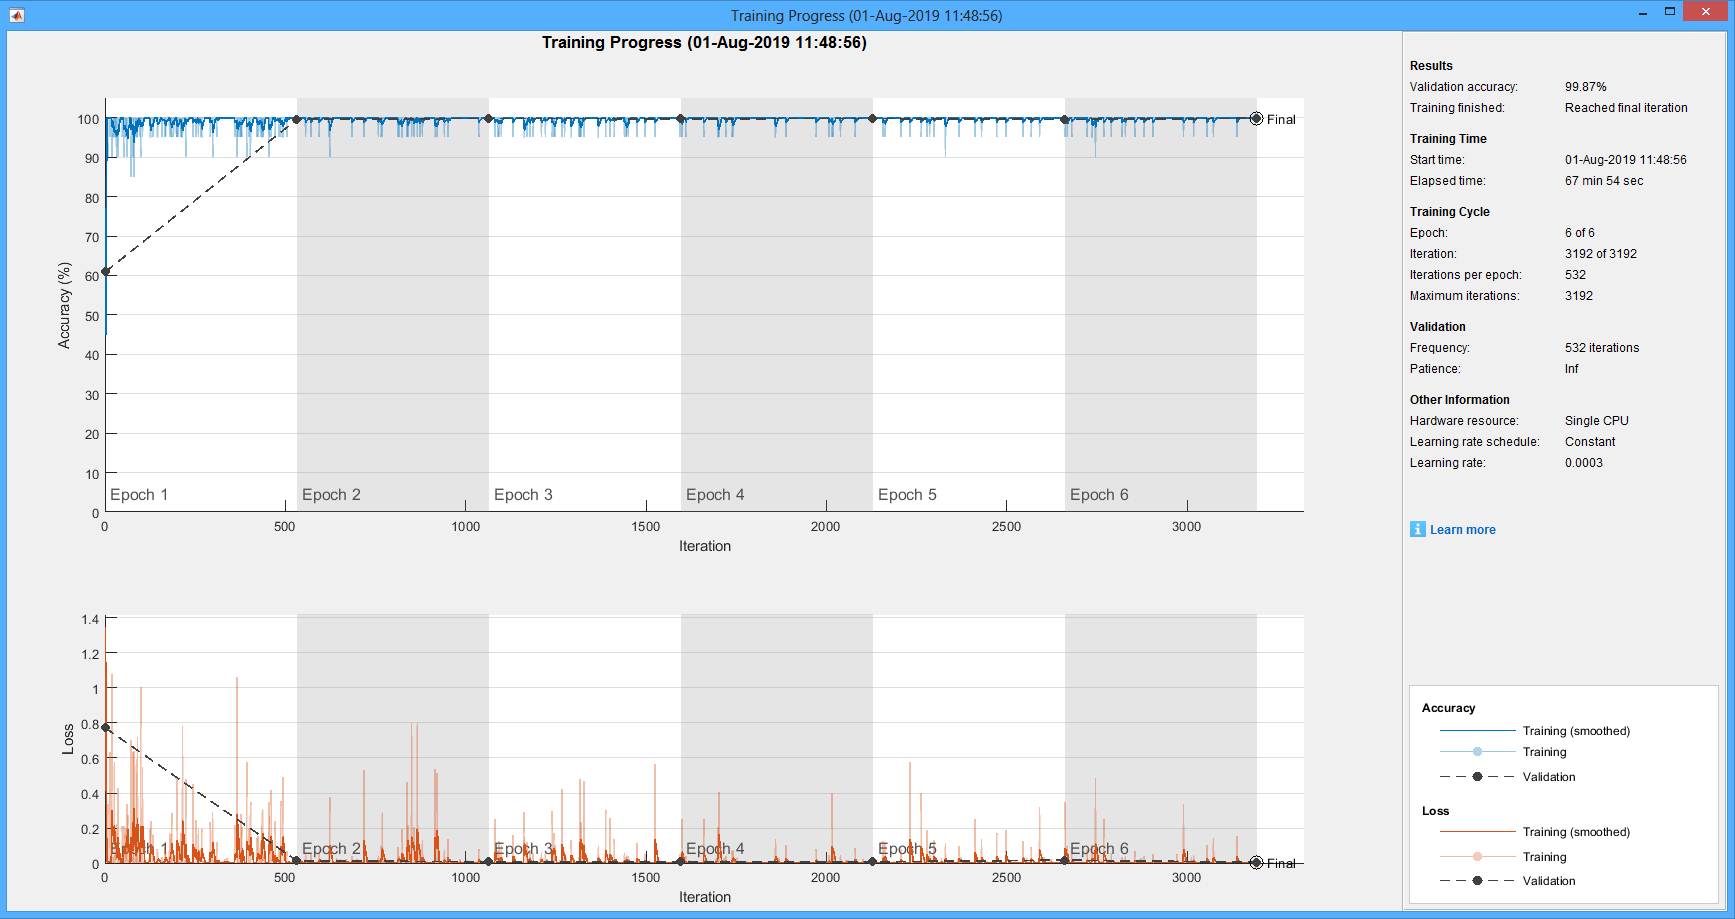
\includegraphics[width=0.88\textwidth]{TrainingAlexNet.png}
  
  \caption{Grafico del ri-addestramento di AlexNet}
  \label{graficoAlexnet}

\end{figure}

\begin{figure}[h!]
  \centering
  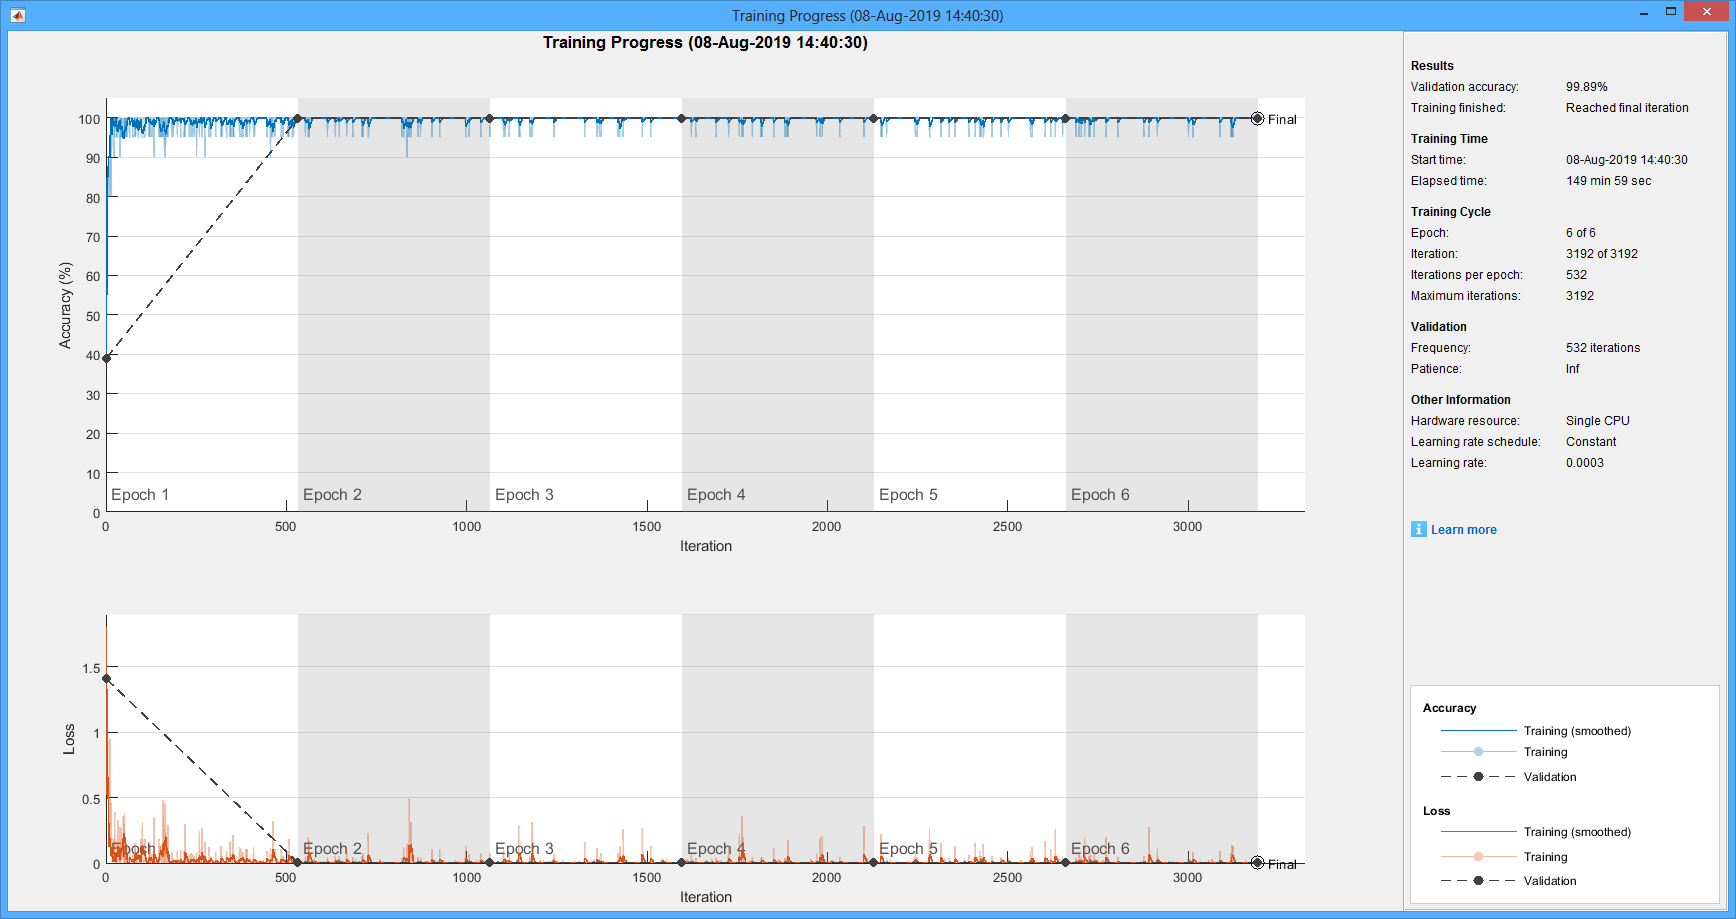
\includegraphics[width=0.88\textwidth]{TrainingGoogLeNet.png}
  
  \caption{Grafico del ri-addestramento di GoogLeNet}
  \label{graficoGooglenet}

\end{figure}

\begin{figure}[h!]
  \centering
  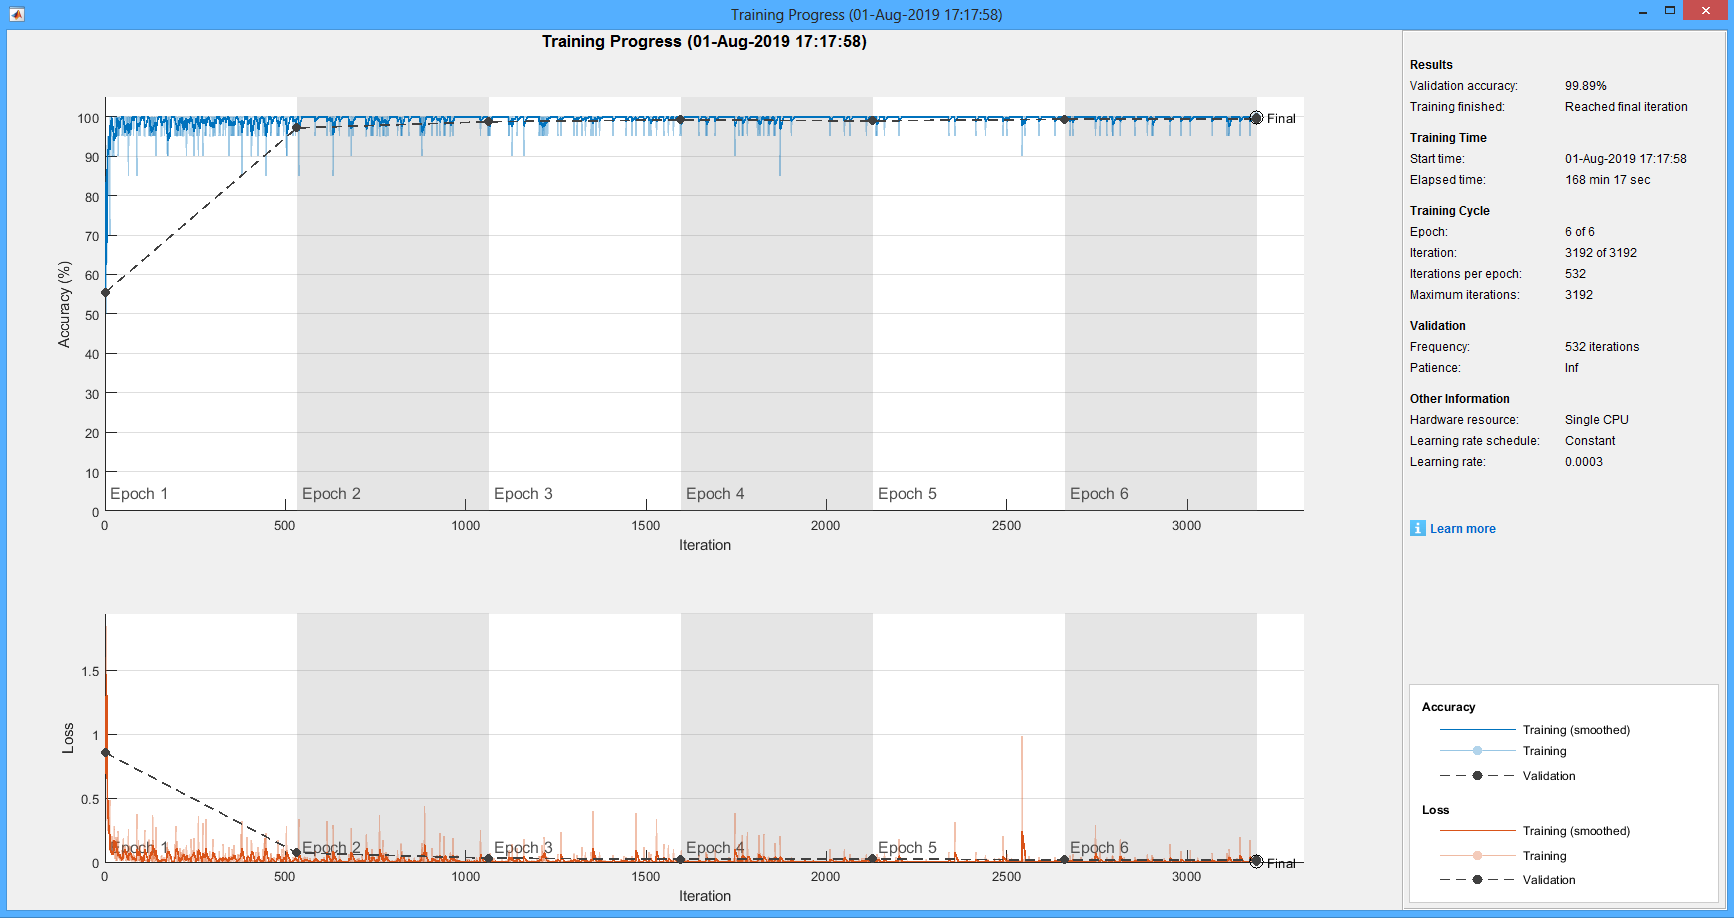
\includegraphics[width=0.88\textwidth]{TrainingResNet18.png}
  
  \caption{Grafico del ri-addestramento di ResNet-18}
  \label{graficoResnet18}

\end{figure}

\begin{figure}[h!]
  \centering
  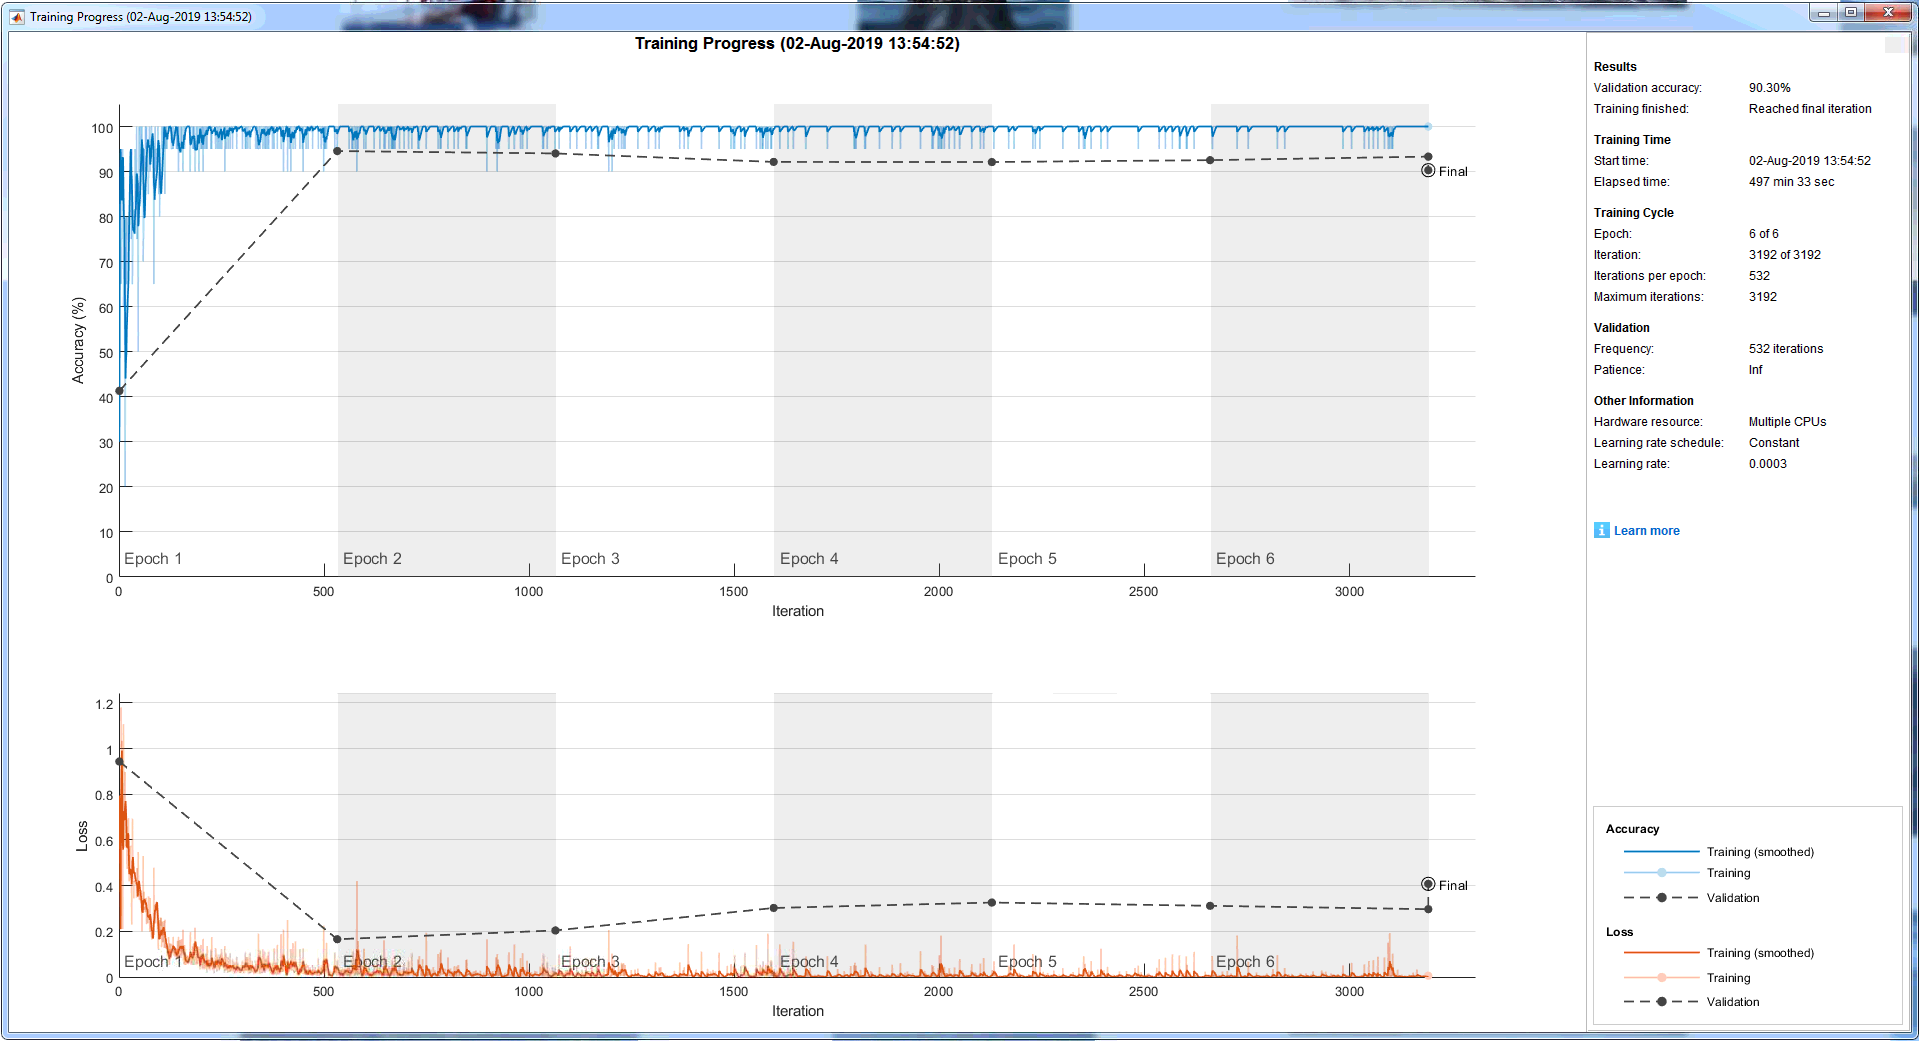
\includegraphics[width=0.88\textwidth]{TrainingResNet50.png}
  
  \caption{Grafico del ri-addestramento di ResNet-50.  Si noti che la \textit{training accuracy} è prossima al 100\% mentre la \textit{validation accuracy} si attesta al 90\%, chiaro sintomo di \textit{overfitting} al training set}
  \label{graficoResnet50}

\end{figure}

Con la sola esclusione di ResNet-50, i valori di accuratezza ottenuti, calcolati sul \textit{validation set}, sono molto elevati. Il successo ottenuto da questi classificatori nel risolvere il problema di classificazione delle pinne è dovuto probabilmente alla facilità con cui la rete riesce ad adattarsi al nuovo dominio di applicazione (d'altronde, è una classificazione binaria abbastanza semplice, a maggior ragione per reti molto profonde in grado di risolvere problemi di classificazione ben più complessi). Diverso è il caso di ResNet-50: per quanto comunque alta, l'accuratezza raggiunta del 90.30\% non è paragonabile a quella delle rimanenti tre reti. Si avanza quindi l'ipotesi di \textit{overfitting} della rete al \textit{training set}. Questa ipotesi è corroborata dal fatto che l'accuratezza valutata sul \textit{training set} è invece prossima al 100\%, come si nota in fig. \ref{graficoResnet50}. Questa mancata capacità di generalizzazione può essere conseguenza dell'eccessiva complessità della rete (n. di parametri inutilmente elevato), in rapporto ad un \textit{training set} relativamente piccolo\footnote{Delle considerazioni simili sono state fatte anche nel paper originale di ResNet \cite{resnet}.}.\\

Le performance delle quattro reti sono state, inoltre, misurate sul dataset dei ritagli ottenuti con CropFin v1 dal dataset degli scatti nelle Azzorre, di dimensione $n=20395$ (usato quindi come \textit{test set}). Si ricorda che questi ritagli erano stati in precedenza etichettati manualmente, come descritto nel par. \ref{faseClassificazione}. I risultati sono riassunti in tabella \ref{prestazioniRetiAzzorre}.

\begin{table}[h]

  \centering
  \begin{adjustbox}{width=1\textwidth}
  %\small
  \begin{tabular}{c c c c c c c c c}
  \hline
  Rete&Accuracy&Sensitivity&Specificity&TP&FP&TN&FN\\
  \hline
  AlexNet&97.1\%&97.9\%&96.9\%&3712&511&16091&81\\
  GoogLeNet&97.2\%&98.0\%&97.0\%&3718&493&16109&75\\
  ResNet-18&96.7\%&99.0\%&96.3\%&3754&619&15983&39\\
  ResNet-50&77.9\%&98.1\%&73.3\%&3722&4431&12171&71\\
  \hline
  \end{tabular}
  \end{adjustbox}
  
  \caption{Prestazioni valutate sul dataset dei ritagli delle Azzorre, usato come \textit{test set}}
  \label{prestazioniRetiAzzorre}

\end{table}

Come ci si aspettava, le reti hanno prestazioni abbastanza elevate, ad eccezione di ResNet-50. L'inefficienza di quest'ultima rete è aggravata dal fatto che la sua specificity sia risultata bassa: confondere un ritaglio 'No Pinna' con un ritaglio 'Pinna' è, dal punto di vista dell'utente (tipicamente un ricercatore), più grave del contrario. Infatti, è tollerabile perdere qualche pinna nei falsi negativi (in una spedizione uno stesso esemplare è spesso immortalato in più fotografie, quindi c'è un'alta probabilità che le sue pinne siano presenti in più ritagli di cui almeno uno correttamente classificato come 'Pinna'), ma è meno tollerabile avere molti falsi positivi (infatti gli algoritmi di foto-identificazione delle pinne come quello proposto in \cite{emanuele} danno sempre in output un \textit{match} plausibile, anche se l'input non raffigura una pinna).

Per questo motivo, d'ora in avanti ResNet-50 non verrà più utilizzata.

\subsection{Classificatore ensemble}
\label{classEnsemble}
Al fine di migliorare ulteriormente l'accuratezza della classificazione, si è sperimentato un metodo di apprendimento ensemble (\textit{ensemble learning}, par. \ref{ensemble}). L'idea chiave è quella di creare un insieme (\textit{ensemble}) di classificatori, ciascuno dei quali è chiamato a "votare" circa l'esito della predizione; a seconda dello "schema di consenso" (\textit{consensus scheme}) scelto per l'ensemble, cioè a seconda di quanto peso assume ciascun voto nella classificazione finale, l'output complessivo sarà la classe che avrà ricevuto "democraticamente" il maggior consenso.

Come già descritto nel par. \ref{ensemble}, l'efficacia dei metodi ensemble è dovuta al fatto che, solitamente, differenti modelli  addestrati per risolvere uno stesso problema di classificazione non faranno tutti gli stessi errori sul \textit{test set} (gli errori si possono cioè considerare, in buona sostanza, incorrelati). Se lo schema di consenso applicato è il \textit{major voting}, si dimostra che l'ensemble di classificatori ha sempre prestazioni migliori o almeno uguali a quelle di ciascuna rete dell'ensemble presa singolarmente; il miglioramento delle prestazioni è tanto migliore quanto più gli errori commessi dalle reti dell'ensemble sono tra loro incorrelati.\cite{dlbook}\cite{ensembles}\\

\noindent L'ensemble utilizzato è costituito dalle reti AlexNet, GoogLeNet e ResNet-18, addestrate sul dataset dei ritagli di Taranto. Uno schema dell'ensemble è raffigurato in fig. \ref{fig:ensemble}

\begin{figure}[h]
\centering
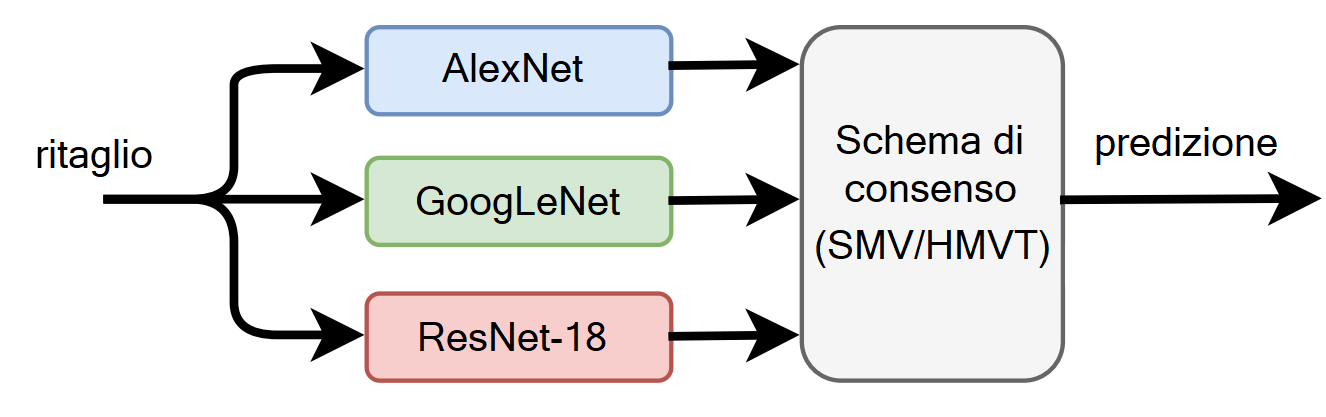
\includegraphics[width=0.8\textwidth]{ensemble.png}
\caption{Schema del classificatore ensemble creato}
\label{fig:ensemble}
\end{figure}

Sono stati effettuati due esperimenti che adottano due diversi schemi di consenso, di seguito elencati:

\begin{itemize}

\item \textbf{\textit{soft major voting}}: un ritaglio è classificato come 'Pinna' se la media delle probabilità attribuite alla classe 'Pinna' da ciascuna rete è maggiore del 50\%. La nuova probabilità attribuita alla classe 'Pinna' è appunto la suddetta media. Vale allo stesso modo il viceversa relativamente alla classe 'No Pinna'.

\item \textbf{\textit{hard major voting} con soglia}: un ritaglio è classificato come 'Pinna' se almeno due delle tre reti lo classificano come 'Pinna' e se inoltre la media delle probabilità attribuite alla classe 'Pinna' da ciascuna rete è maggiore di una certa soglia, fissata arbitrariamente al 97\%. La nuova probabilità attribuita alla classe 'Pinna' è appunto la suddetta media. Vale allo stesso modo il viceversa relativamente alla classe 'No Pinna'.

\end{itemize}

Gli esperimenti consistono nella classificazione del \textit{test set} contenente i ritagli delle Azzorre da parte del classificatore ensemble. Questi esperimenti hanno come scopo la misurazione delle prestazioni del classificatore ensemble, e consentono il confronto di prestazioni tra questo nuovo modello e quello di CropFin v1, descritto in \cite{gianvito} (e provato sullo stesso \textit{test set}). I risultati dei due esperimenti sono riportati in tabella \ref{prestazioniEnsemble}, assieme a quello relativo al classificatore nativo in CropFin v1.
Gli stessi dati riportati nella tabella \ref{prestazioniEnsemble} sono mostrati sotto forma di matrici di confusione in fig. \ref{fig:confMatEnsemble}.
In figura \ref{testHMVT} si riportano infine alcuni campioni di ritagli classificati dall'ensemble.\\


\begin{table}[h]

  \centering
  \begin{adjustbox}{width=1\textwidth}
  %\small
  \begin{tabular}{c c c c c c c c c}
  \hline
  Modello&Accuracy&Sensitivity&Specificity&TP&FP&TN&FN\\
  \hline
  Ensemble (SMV)&97.2\%&98.7\%&96.9\%&3745&518&16084&48\\
  Ensemble (HMVT)&97.2\%&93.4\%&98.1\%&3543&313&16289&250\\
  CropFin v1&92\%&85\%&95\%&--&--&--&--\\
  \hline
  \end{tabular}
  \end{adjustbox}
  
  \caption{Prestazioni di differenti modelli di classificazione, valutate sul dataset dei ritagli delle Azzorre. Abbreviazioni: SMV = \textit{soft major voting}, HMVT = \textit{hard major voting} con soglia (\textit{threshold}) sulla probabilità media}
  \label{prestazioniEnsemble}
  %\vspace{10mm}

\end{table}



\begin{figure}[h!]

  \centering
  
  \begin{subfigure}[b]{0.45\textwidth}
  \raggedright
    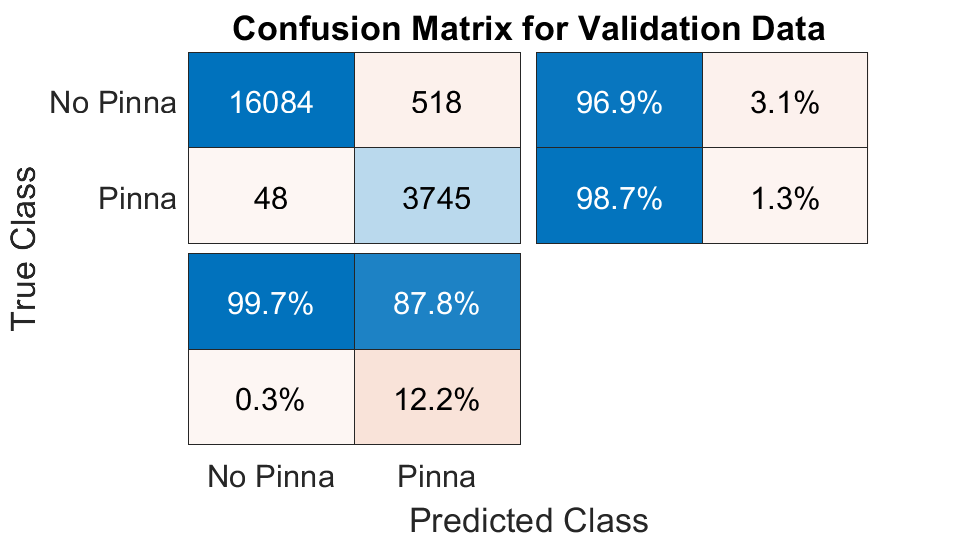
\includegraphics[width=\textwidth]{confMatAzzorreSMV.png}
    \caption{}
  \end{subfigure}
  \begin{subfigure}[b]{0.45\textwidth}
  \raggedleft
    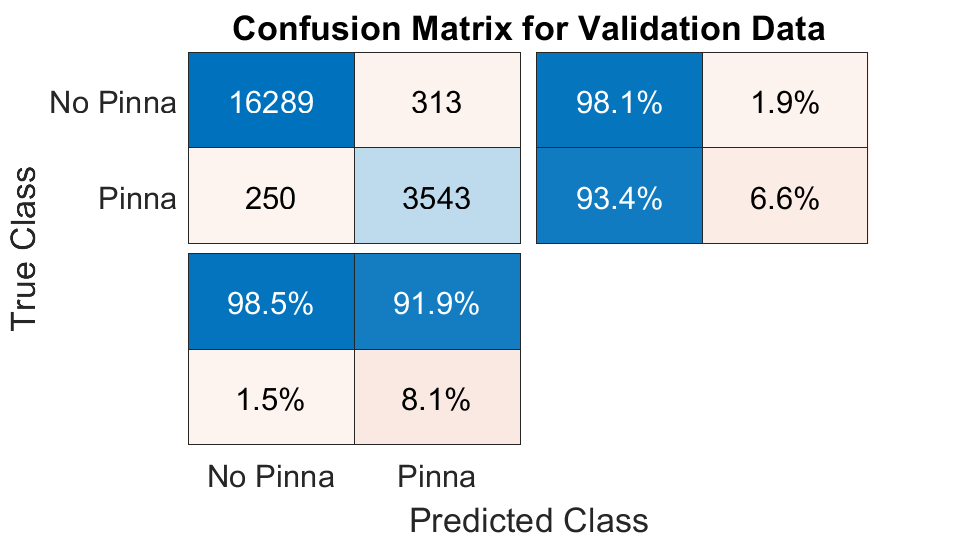
\includegraphics[width=\textwidth]{confMatAzzorreHMVT.png}
    \caption{}
  \end{subfigure}
  
  \caption{Matrici di confusione relative alle predizioni del nuovo ensemble sui ritagli delle Azzorre, con schema di consenso (a) \textit{soft major voting}, (b) \textit{hard major voting} con soglia.}
  \label{fig:confMatEnsemble}
\end{figure}


\begin{figure}[h]
\centering
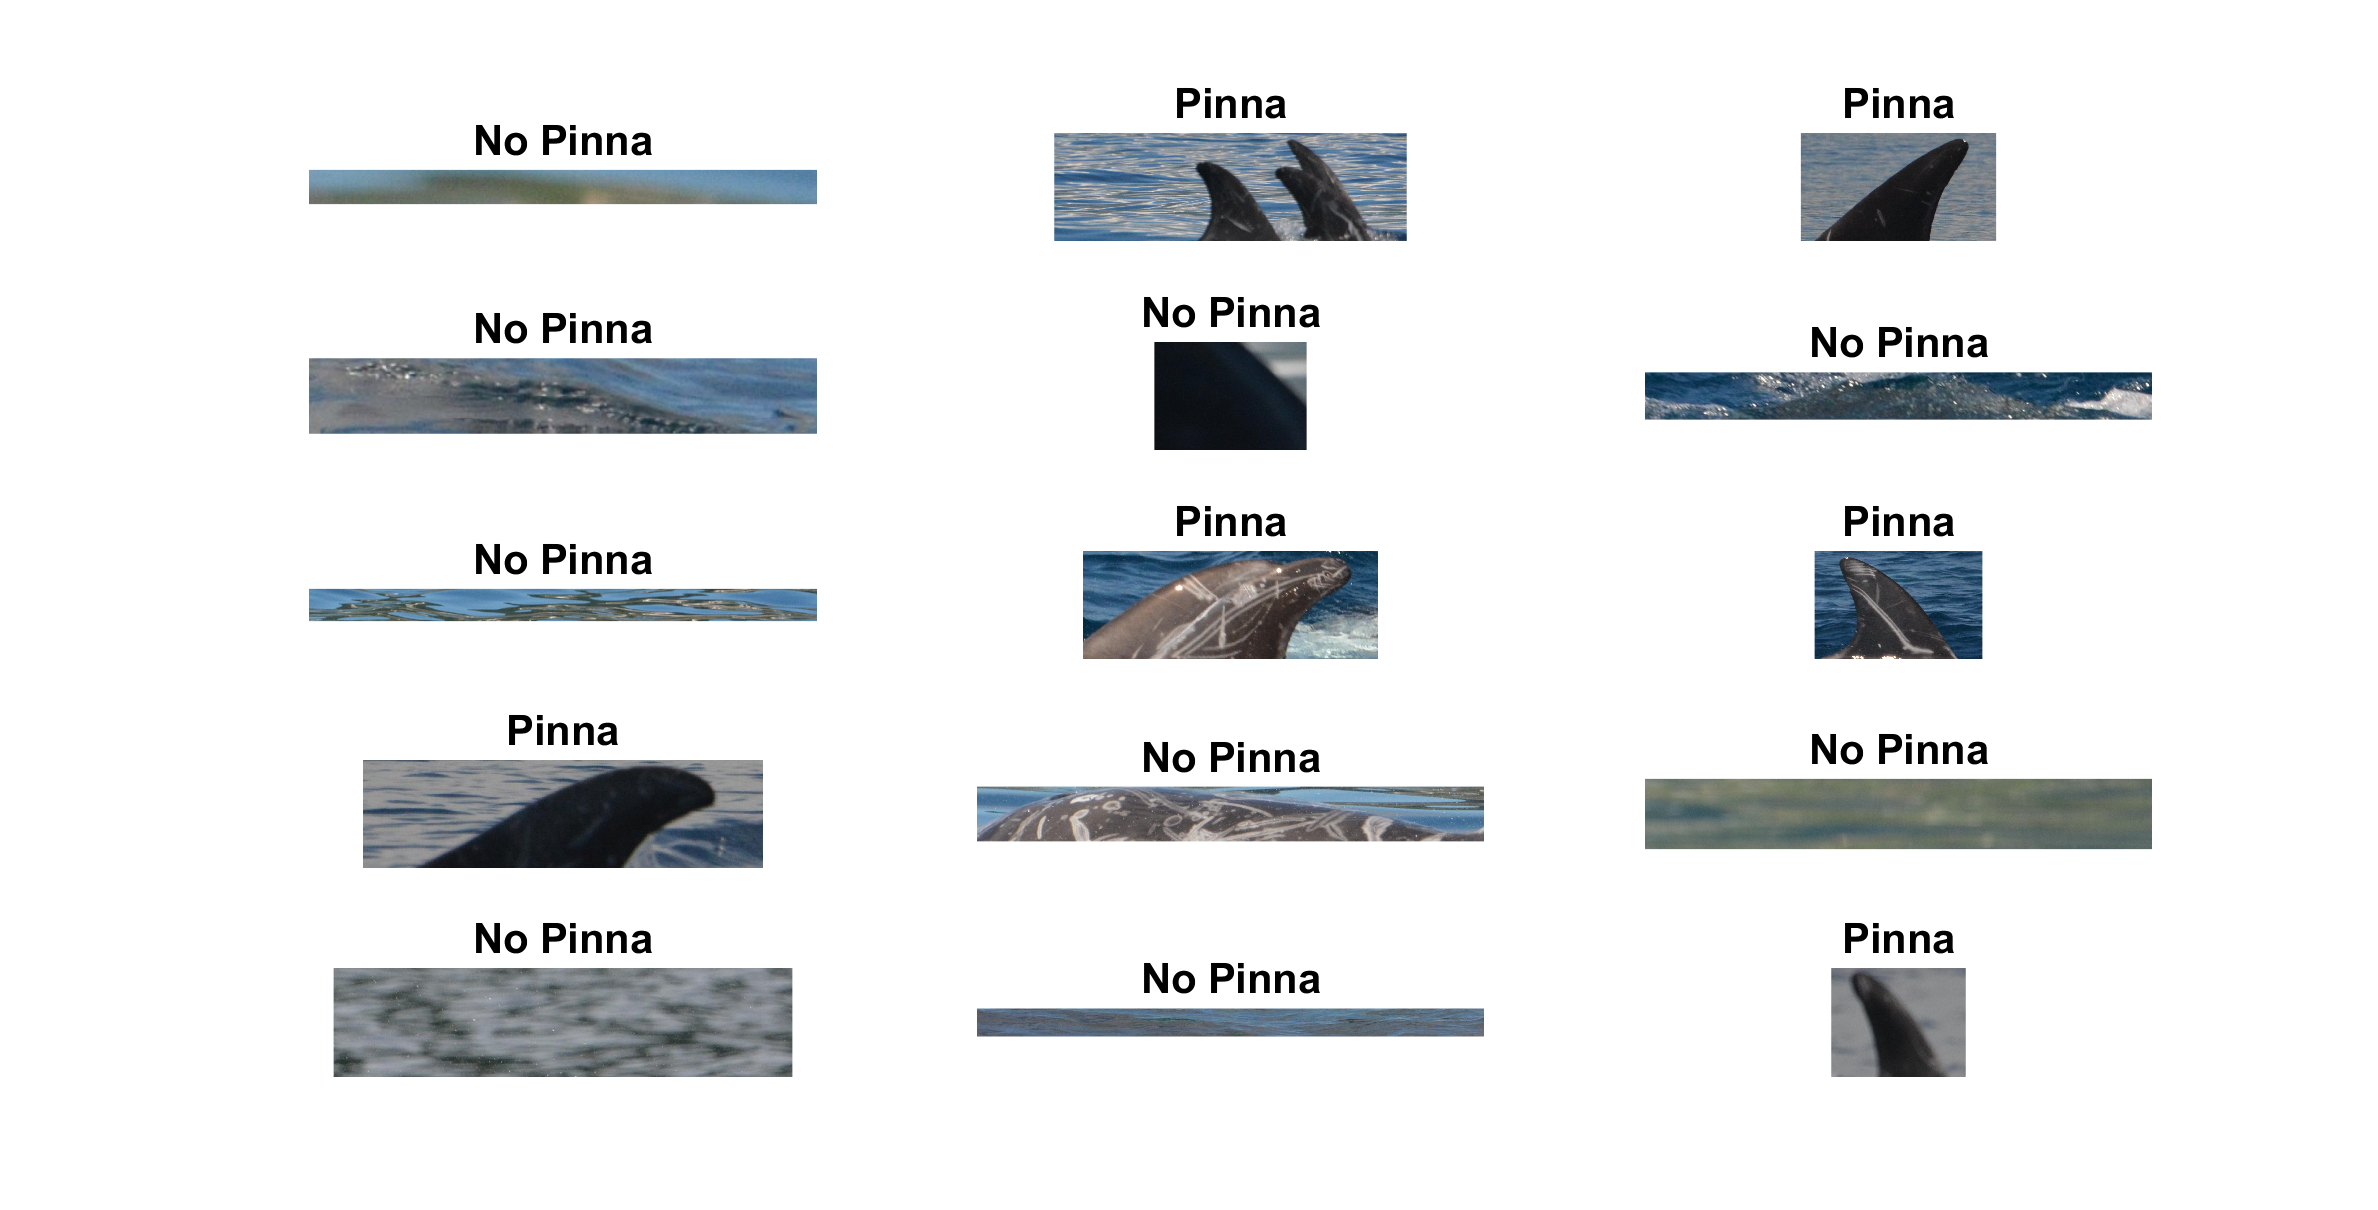
\includegraphics[width=\textwidth]{testHMVT.png}
\caption{Alcune predizioni proposte dall'ensemble con schema di consenso HMVT. Si noti ad esempio quella centrale in alto: compaiono tre pinne di cui addirittura due sovrapposte, ma il classificatore restituisce 'Pinna'. Sebbene il classificatore sia riuscito a confermare la presenza di una pinna, l'etichetta corretta era 'No Pinna' (per i criteri di etichettatura adottati sui ritagli con pinne multiple). Evidentemente nel training set con i ritagli di Taranto non erano presenti molti ritagli con pinne multiple, quindi il classificatore ha avuto difficoltà ad attribuire la classe 'No Pinna' a questo tipo di ritagli.}
\label{testHMVT}
\end{figure}


Confrontando le prestazioni ottenute dal classificatore di CropFin v1 e i due classificatori ensemble creati sfruttando il principio del \textit{transfer learning} è evidente la maggiore efficienza di questi ultimi, in tutti i parametri messi a confronto.

Si fa notare infine che lo schema di consenso di tipo HMVT ha fatto registrare un miglioramento del parametro di \textit{specificity} che, come spiegato in precedenza, è un parametro fondamentale in quanto dà una misura di quanto i ritagli classificati come 'Pinna' sono "sporcati" da ritagli 'No Pinna' erroneamente classificati come 'Pinna', un errore che l'utente finale vorrebbe evitare. Si può verificare che alzando la soglia sopra il 97\% la \textit{specificity} aumenta ancora, ma a scapito della \textit{sensitivity}, che decresce con una velocità purtroppo maggiore della \textit{specificity}. Tuttavia questo non costituisce un grosso problema nel caso in cui, come spesso avviene, ci sia una discreta ridondanza nella presenza di uno stesso esemplare in più foto di una stessa spedizione in mare, come descritto in precedenza\footnote{In questo caso, infatti, è meno probabile che in un dataset di ritagli da scatti avvenuti in una specifica spedizione vengano scartati \emph{tutti} i ritagli relativi alla pinna di un certo esemplare}.

In conclusione, quindi, si può affermare che adattare al nostro task di classificazione di ritagli di pinne un'opportuna rete neurale convoluzionale pre-addestrata con il metodo del \textit{transfer learning} piuttosto che costruirne una \textit{from scratch} è risultato vantaggioso in termini di prestazioni offerte ed è quindi servito a migliorare la fase di classificazione di CropFin v1. Inoltre, si è verificato che le prestazioni aumentano ulteriormente costruendo un classificatore di tipo \textit{ensemble} che raccolga diverse reti ri-addestrate che lavorino in sinergia attraverso uno schema di consenso di \textit{major voting}.
Il miglioramento della fase di classificazione, e soprattutto del parametro della \textit{specificity}, è fondamentale in vista di una successiva applicazione di un algoritmo di foto-identificazione delle pinne, ad esempio quello descritto in \cite{emanuele}.
Per i motivi descritti, questo nuovo classificatore è preferibile a quello di CropFin v1.

Il tempo di addestramento è risultato molto più alto di quello del classificatore di CropFin v1, pur avendo disposto di capacità di calcolo di gran lunga superiore.
Inoltre, l'occupazione di memoria del nuovo ensemble ($\sim$263 MB) è più di 8 volte superiore a quella del classificatore \textit{ad-hoc} di CropFin v1 ($\sim$31,2 MB).
Il tempo di addestramento e l'occupazione di memoria elevati sono comunque "ripagati" dalle alte prestazioni dell'ensemble di reti.
Tuttavia non c'è un criterio oggettivo per valutare quantitativamente l'utilità di questo miglioramento di prestazioni in rapporto all'allungamento del tempo di addestramento e all'aumento di occupazione di memoria del classificatore.

Si è infine potuto verificare che il tempo che l'ensemble impiega per effettuare una predizione su un ritaglio è leggermente più alto a quello impiegato dal classificatore di CropFin v1.

I problemi evidenziati, soprattutto per quanto concerne le dimensioni del classificatore e il tempo necessario ad effettuare una predizione (requisiti fondamentali per agevolare il lavoro del biologo) sono però quasi ininfluenti su una macchina dal discreto potere computazionale e memoria disponibile.\\

\noindent I motivi sopracitati rendono il nuovo classificatore ensemble preferibile a quello nativo di CropFin v1.